% Options for packages loaded elsewhere
\PassOptionsToPackage{unicode}{hyperref}
\PassOptionsToPackage{hyphens}{url}
%
\documentclass[
  11pt]{report}
\usepackage{amsmath,amssymb}
\usepackage{lmodern}
\usepackage{iftex}
\ifPDFTeX
  \usepackage[T1]{fontenc}
  \usepackage[utf8]{inputenc}
  \usepackage{textcomp} % provide euro and other symbols
\else % if luatex or xetex
  \usepackage{unicode-math}
  \defaultfontfeatures{Scale=MatchLowercase}
  \defaultfontfeatures[\rmfamily]{Ligatures=TeX,Scale=1}
\fi
% Use upquote if available, for straight quotes in verbatim environments
\IfFileExists{upquote.sty}{\usepackage{upquote}}{}
\IfFileExists{microtype.sty}{% use microtype if available
  \usepackage[]{microtype}
  \UseMicrotypeSet[protrusion]{basicmath} % disable protrusion for tt fonts
}{}
\makeatletter
\@ifundefined{KOMAClassName}{% if non-KOMA class
  \IfFileExists{parskip.sty}{%
    \usepackage{parskip}
  }{% else
    \setlength{\parindent}{0pt}
    \setlength{\parskip}{6pt plus 2pt minus 1pt}}
}{% if KOMA class
  \KOMAoptions{parskip=half}}
\makeatother
\usepackage{xcolor}
\IfFileExists{xurl.sty}{\usepackage{xurl}}{} % add URL line breaks if available
\IfFileExists{bookmark.sty}{\usepackage{bookmark}}{\usepackage{hyperref}}
\hypersetup{
  pdftitle={Probabilidade e Estatística com R},
  pdfauthor={Fernando Náufel},
  pdflang={pt-br},
  hidelinks,
  pdfcreator={LaTeX via pandoc}}
\urlstyle{same} % disable monospaced font for URLs
\usepackage[margin=1in]{geometry}
\usepackage{color}
\usepackage{fancyvrb}
\newcommand{\VerbBar}{|}
\newcommand{\VERB}{\Verb[commandchars=\\\{\}]}
\DefineVerbatimEnvironment{Highlighting}{Verbatim}{commandchars=\\\{\}}
% Add ',fontsize=\small' for more characters per line
\usepackage{framed}
\definecolor{shadecolor}{RGB}{248,248,248}
\newenvironment{Shaded}{\begin{snugshade}}{\end{snugshade}}
\newcommand{\AlertTok}[1]{\textcolor[rgb]{0.94,0.16,0.16}{#1}}
\newcommand{\AnnotationTok}[1]{\textcolor[rgb]{0.56,0.35,0.01}{\textbf{\textit{#1}}}}
\newcommand{\AttributeTok}[1]{\textcolor[rgb]{0.77,0.63,0.00}{#1}}
\newcommand{\BaseNTok}[1]{\textcolor[rgb]{0.00,0.00,0.81}{#1}}
\newcommand{\BuiltInTok}[1]{#1}
\newcommand{\CharTok}[1]{\textcolor[rgb]{0.31,0.60,0.02}{#1}}
\newcommand{\CommentTok}[1]{\textcolor[rgb]{0.56,0.35,0.01}{\textit{#1}}}
\newcommand{\CommentVarTok}[1]{\textcolor[rgb]{0.56,0.35,0.01}{\textbf{\textit{#1}}}}
\newcommand{\ConstantTok}[1]{\textcolor[rgb]{0.00,0.00,0.00}{#1}}
\newcommand{\ControlFlowTok}[1]{\textcolor[rgb]{0.13,0.29,0.53}{\textbf{#1}}}
\newcommand{\DataTypeTok}[1]{\textcolor[rgb]{0.13,0.29,0.53}{#1}}
\newcommand{\DecValTok}[1]{\textcolor[rgb]{0.00,0.00,0.81}{#1}}
\newcommand{\DocumentationTok}[1]{\textcolor[rgb]{0.56,0.35,0.01}{\textbf{\textit{#1}}}}
\newcommand{\ErrorTok}[1]{\textcolor[rgb]{0.64,0.00,0.00}{\textbf{#1}}}
\newcommand{\ExtensionTok}[1]{#1}
\newcommand{\FloatTok}[1]{\textcolor[rgb]{0.00,0.00,0.81}{#1}}
\newcommand{\FunctionTok}[1]{\textcolor[rgb]{0.00,0.00,0.00}{#1}}
\newcommand{\ImportTok}[1]{#1}
\newcommand{\InformationTok}[1]{\textcolor[rgb]{0.56,0.35,0.01}{\textbf{\textit{#1}}}}
\newcommand{\KeywordTok}[1]{\textcolor[rgb]{0.13,0.29,0.53}{\textbf{#1}}}
\newcommand{\NormalTok}[1]{#1}
\newcommand{\OperatorTok}[1]{\textcolor[rgb]{0.81,0.36,0.00}{\textbf{#1}}}
\newcommand{\OtherTok}[1]{\textcolor[rgb]{0.56,0.35,0.01}{#1}}
\newcommand{\PreprocessorTok}[1]{\textcolor[rgb]{0.56,0.35,0.01}{\textit{#1}}}
\newcommand{\RegionMarkerTok}[1]{#1}
\newcommand{\SpecialCharTok}[1]{\textcolor[rgb]{0.00,0.00,0.00}{#1}}
\newcommand{\SpecialStringTok}[1]{\textcolor[rgb]{0.31,0.60,0.02}{#1}}
\newcommand{\StringTok}[1]{\textcolor[rgb]{0.31,0.60,0.02}{#1}}
\newcommand{\VariableTok}[1]{\textcolor[rgb]{0.00,0.00,0.00}{#1}}
\newcommand{\VerbatimStringTok}[1]{\textcolor[rgb]{0.31,0.60,0.02}{#1}}
\newcommand{\WarningTok}[1]{\textcolor[rgb]{0.56,0.35,0.01}{\textbf{\textit{#1}}}}
\usepackage{longtable,booktabs,array}
\usepackage{calc} % for calculating minipage widths
% Correct order of tables after \paragraph or \subparagraph
\usepackage{etoolbox}
\makeatletter
\patchcmd\longtable{\par}{\if@noskipsec\mbox{}\fi\par}{}{}
\makeatother
% Allow footnotes in longtable head/foot
\IfFileExists{footnotehyper.sty}{\usepackage{footnotehyper}}{\usepackage{footnote}}
\makesavenoteenv{longtable}
\usepackage{graphicx}
\makeatletter
\def\maxwidth{\ifdim\Gin@nat@width>\linewidth\linewidth\else\Gin@nat@width\fi}
\def\maxheight{\ifdim\Gin@nat@height>\textheight\textheight\else\Gin@nat@height\fi}
\makeatother
% Scale images if necessary, so that they will not overflow the page
% margins by default, and it is still possible to overwrite the defaults
% using explicit options in \includegraphics[width, height, ...]{}
\setkeys{Gin}{width=\maxwidth,height=\maxheight,keepaspectratio}
% Set default figure placement to htbp
\makeatletter
\def\fps@figure{htbp}
\makeatother
% Make links footnotes instead of hotlinks:
\DeclareRobustCommand{\href}[2]{#2\footnote{\url{#1}}}
\setlength{\emergencystretch}{3em} % prevent overfull lines
\providecommand{\tightlist}{%
  \setlength{\itemsep}{0pt}\setlength{\parskip}{0pt}}
\setcounter{secnumdepth}{5}
\ifLuaTeX
\usepackage[bidi=basic]{babel}
\else
\usepackage[bidi=default]{babel}
\fi
\babelprovide[main,import]{brazilian}
% get rid of language-specific shorthands (see #6817):
\let\LanguageShortHands\languageshorthands
\def\languageshorthands#1{}

\hypersetup{
  colorlinks,
  breaklinks,
  linkcolor=magenta,
  urlcolor=blue
}

% Lexend font
\usepackage{lexend}


% Para bibliografia em português
\usepackage{babelbib}

% Para títulos de capítulos e seções:
\usepackage[nobottomtitles*]{titlesec}

%%%%%%%%%%%%%%%
%
% Titulos de capítulos e seções

\titleformat{\chapter}[display]%
{\bfseries\Large}%
{\filleft\MakeUppercase{\chaptertitlename} \Huge\thechapter}%
{4ex}%
{\titlerule%
  \vspace{2ex}%
  \filright}%
[\vspace{2ex}%
\titlerule%
\vspace{10ex}]

\titleformat{\section}[block]%
{\bfseries\Large}%
{\thesection}{.5em}{\titlerule\\[.8ex]\bfseries}

\titleformat{\subsection}[block]%
{\bfseries}%
{\thesubsection}{.5em}{\titlerule\\[.8ex]\bfseries}%
[\vspace{1ex}]

%%%%%%%%%%%%%%%
%
% Caixas

\usepackage{tcolorbox}

\tcbset{
  rounded corners,
  boxrule=0.3mm,
  colback=black!.5!white,
  parbox=false
}

\newtcolorbox{rmdbox}{
  colframe=black!40!white,
}


\newtcolorbox{mycaution}{
  colframe=red!75!black,
  sidebyside,
  lower separated=false,
  lefthand width=1cm,
  sidebyside gap=4mm
}

\newenvironment{rmdcaution}
{
  \begin{mycaution}
    
\includegraphics{images/caution.png}
    \tcblower
  }
  {
  \end{mycaution}
}

\newtcolorbox{myimportant}{
  colframe=green!75!black,
  sidebyside,
  lower separated=false,
  lefthand width=1cm,
  sidebyside gap=4mm
}

\newenvironment{rmdimportant}
{
  \begin{myimportant}
    
\includegraphics{images/important.png}
    \tcblower
  }
  {
  \end{myimportant}
}

\newtcolorbox{mywarning}{
  colframe=yellow!80!black,
  sidebyside,
  lower separated=false,
  lefthand width=1cm,
  sidebyside gap=4mm
}

\newenvironment{rmdwarning}
{
  \begin{mywarning}
    
\includegraphics{images/warning.png}
    \tcblower
  }
  {
  \end{mywarning}
}

\newtcolorbox{mynote}{
  colframe=yellow!70!black,
  sidebyside,
  lower separated=false,
  lefthand width=1cm,
  sidebyside gap=4mm
}

\newenvironment{rmdnote}
{
  \begin{mynote}
    
\includegraphics{images/note.png}
    \tcblower
  }
  {
  \end{mynote}
}

\newtcolorbox{mytip}{
  colframe=blue!50!white,
  sidebyside,
  lower separated=false,
  lefthand width=1cm,
  sidebyside gap=4mm
}

\newenvironment{rmdtip}
{
  \begin{mytip}
    
\includegraphics{images/tip.png}
    \tcblower
  }
  {
  \end{mytip}
}

% For highlighting using \hl{}
\usepackage{soul}


% Code chunks and output
\usepackage[framemethod=pgf]{mdframed}
\renewenvironment{Shaded}{
  \begin{mdframed}[%
    roundcorner=2pt,%
    innerleftmargin=5pt,%
    innerrightmargin=5pt,%
    topline=true,%
    leftline=true,%
    rightline=true,%
    bottomline=true,%
    linewidth=0.5pt,%
    linecolor=black!20,%
    backgroundcolor=black!2,%
    skipabove=2ex,%
    skipbelow=2.5ex%
  ]%
}
{
  \end{mdframed}
}

% End of preamble for bookdowntemplate01

%%%%%%%%%%%%%%%%%%%%%%%%%%%%%%%%%%%%%%%%%%%%%%%%%%%%%%

\usepackage{booktabs}
\usepackage{longtable}
\usepackage{array}
\usepackage{multirow}
\usepackage{wrapfig}
\usepackage{float}
\usepackage{colortbl}
\usepackage{pdflscape}
\usepackage{tabu}
\usepackage{threeparttable}
\usepackage{threeparttablex}
\usepackage[normalem]{ulem}
\usepackage{makecell}
\usepackage{xcolor}
\ifLuaTeX
  \usepackage{selnolig}  % disable illegal ligatures
\fi
\usepackage[]{natbib}
\bibliographystyle{apalike}

\title{Probabilidade e Estatística com R}
\author{Fernando Náufel}
\date{(versão de 24/11/2021)}

\begin{document}
\maketitle

{
\setcounter{tocdepth}{1}
\tableofcontents
}
\hypertarget{apresentacao}{%
\chapter*{Apresentação}\label{apresentacao}}
\addcontentsline{toc}{chapter}{Apresentação}

\begin{rmdcaution}
\textbf{Atenção}

Este material ainda está em construção.

Pode haver mudanças a qualquer momento.

Verifique, no rodapé da página \emph{web} ou na capa do arquivo pdf, a data desta versão.

\end{rmdcaution}

\newpage

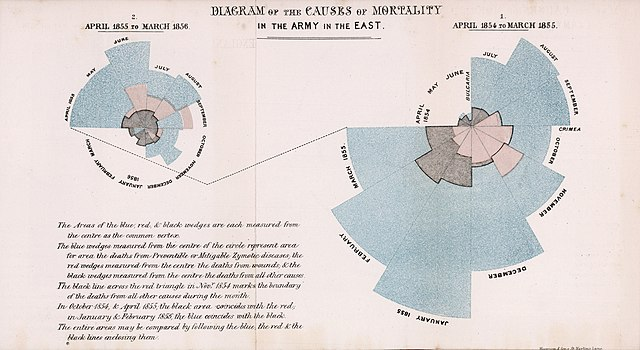
\includegraphics{images/640px-Nightingale-mortality.jpg}

\vspace{2cm}

Este livro/\emph{site} foi iniciado em 2020, durante a pandemia de COVID-19, quando a Universidade Federal Fluminense (UFF) funcionou em regime de ensino remoto durante mais de um ano.

Para atender os alunos do curso de Probabilidade e Estatística do curso de graduação em Ciência da Computação da UFF, decidi gravar aulas em vídeo e disponibilizar os arquivos usados nelas. Foram esses arquivos que deram origem a este livro/\emph{site}.

Este livro/\emph{site} foi construído para pessoas que já saibam programar, embora não necessariamente em R.

Para tirar o máximo proveito deste material, você deve fazer o seguinte:

\begin{enumerate}
\def\labelenumi{\arabic{enumi}.}
\item
  Assistir aos vídeos contidos em cada capítulo. A \emph{playlist} completa está em \url{https://www.youtube.com/playlist?list=PL7SRLwLs7ocaV-Y1vrVU3W7mZnnS0qkWV}.
\item
  Instalar o R no seu computador ou abrir uma conta no RStudio Cloud, para poder usar o R \emph{online}. Você encontra instruções para fazer isto no \protect\hyperlink{rintro}{capítulo de introdução a R}.
\item
  Baixar, \href{https://github.com/fnaufel/probestr}{neste repositório do Github}, o código-fonte deste livro/\emph{site}, para poder rodar e alterar os exemplos.
\item
  Seguir os \emph{links} para outras fontes \emph{online} que abordam assuntos que não são cobertos em detalhes neste curso.
\item
  Fazer os exercícios. Ao longo do tempo, acrescentarei \emph{links} para vídeos explicando as soluções.
\end{enumerate}

\begin{rmdimportant}
{\hl{Se você estiver lendo este material na \emph{web}, você pode clicar nos comandos e funções que aparecem nos blocos de código em R}} para abrir páginas da documentação sobre eles.

Se você preferir ler este livro em pdf, ou se quiser imprimi-lo, \href{https://github.com/fnaufel/probestr/blob/master/docs/probestr.pdf}{faça o \emph{download} do arquivo aqui}.

\end{rmdimportant}

\hypertarget{refrec}{%
\section*{Referências recomendadas}\label{refrec}}
\addcontentsline{toc}{section}{Referências recomendadas}

\hypertarget{em-portuguuxeas}{%
\subsection*{Em português}\label{em-portuguuxeas}}
\addcontentsline{toc}{subsection}{Em português}

\begin{itemize}
\item
  Sillas Gonzaga, \emph{Introdução a R para Visualização e Apresentação de Dados},
  \url{http://sillasgonzaga.com/material/curso_visualizacao/index.html}
\item
  Allan Vieira de Castro Quadros, \emph{Introdução à Análise de Dados em R utilizando Tidyverse}, \url{https://allanvc.github.io/book_IADR-T/}
\item
  Paulo Felipe de Oliveira, Saulo Guerra, Robert McDonnel, \emph{Ciência de Dados com R -- Introdução}, \url{https://cdr.ibpad.com.br/index.html}
\item
  Curso R, \emph{Ciência de Dados em R}, \url{https://livro.curso-r.com/}
\end{itemize}

\hypertarget{em-ingluxeas}{%
\subsection*{Em inglês}\label{em-ingluxeas}}
\addcontentsline{toc}{subsection}{Em inglês}

\begin{itemize}
\item
  Garrett Grolemund, Hadley Wickham, \emph{R for Data Science}, \url{https://r4ds.had.co.nz/}
\item
  Chester Ismay, Albert Y. Kim, \emph{A ModernDive into R and the Tidyverse}, \url{https://moderndive.com/}
\end{itemize}

\hypertarget{exercuxedcio}{%
\section*{Exercício}\label{exercuxedcio}}
\addcontentsline{toc}{section}{Exercício}

\begin{enumerate}
\def\labelenumi{\arabic{enumi}.}
\tightlist
\item
  Pesquise sobre a imagem do início deste capítulo. Ela foi criada em 1858 por Florence Nightingale.
\end{enumerate}

\hypertarget{oque}{%
\chapter{O Que É Estatística?}\label{oque}}

\hypertarget{vuxeddeo-1}{%
\section{Vídeo 1}\label{vuxeddeo-1}}

\begin{center} \url{https://youtu.be/6Q_XSoLCIpc} \end{center}

\hypertarget{exercuxedcios}{%
\section{Exercícios}\label{exercuxedcios}}

\begin{enumerate}
\def\labelenumi{\arabic{enumi}.}
\item
  Você está interessado em estimar a altura de todos os homens da sua faculdade. Para isso, você decide medir as alturas de todos os homens da sua turma de Estatística.

  \begin{itemize}
  \tightlist
  \item
    Qual é a amostra?
  \item
    Qual é a população?
  \end{itemize}
\item
  Um instituto de pesquisa entrevista um grupo de $1000$ pessoas, perguntando a cada uma se ela vai votar a favor do candidato $A$ na próxima eleição. Dos entrevistados, $600$ responderam que sim. A proporção $0{,}6$ (ou $60\%$) é uma estatística ou um parâmetro?
\item
  Você vê alguma diferença entre as cinco situações abaixo? Quais das situações são equivalentes em termos da probabilidade de conseguir $10$ cartas do mesmo naipe?

  \begin{enumerate}
  \def\labelenumii{\alph{enumii}.}
  \item
    Usando um baralho normal, você retira $10$ cartas e registra as cartas retiradas.
  \item
    Usando um baralho normal, você repete a seguinte sequência de ações $10$ vezes: retirar uma carta do baralho, registrar a carta retirada e repor a carta no baralho.
  \item
    Usando uma caixa contendo todas as cartas de $1$ milhão de baralhos reunidos, você retira $10$ cartas e registra as cartas retiradas.
  \item
    Usando uma caixa contendo todas as cartas de $1$ milhão de baralhos reunidos, você repete a seguinte sequência de ações $10$ vezes: retirar uma carta da caixa, registrar a carta retirada e repor a carta na caixa.
  \item
    Usando um baralho \emph{infinito}, você retira $10$ cartas e registra as cartas retiradas.
  \item
    Usando um baralho \emph{infinito}, você repete a seguinte sequência de ações $10$ vezes: retirar uma carta do baralho, registrar a carta retirada e repor a carta no baralho.
  \end{enumerate}
\item
  Qual a graça dos quadrinhos na Figura \ref{fig:xkcd-cor}, que também \href{https://youtu.be/6Q_XSoLCIpc?t=1385}{aparecem no vídeo}?

  \begin{figure}

   {\centering 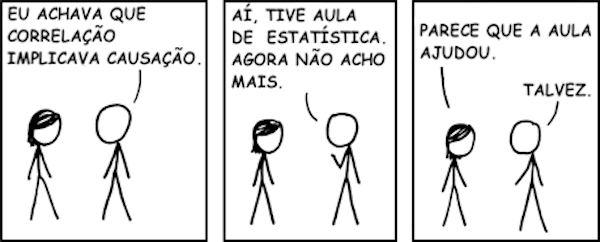
\includegraphics[width=0.9\linewidth]{images/correlation-pt-600} 

   }

   \caption{\url{http://xkcd.com/552/}}\label{fig:xkcd-cor}
   \end{figure}
\item
  Qual a graça dos quadrinhos na Figura \ref{fig:xkcd-blind}?

  \begin{figure}

   {\centering 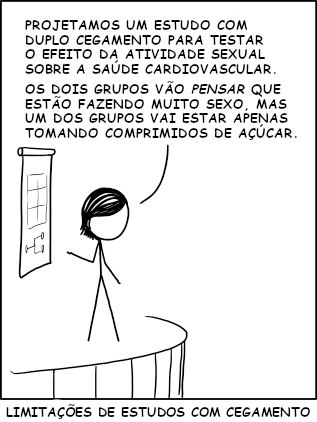
\includegraphics[width=0.5\linewidth]{images/double-blind} 

   }

   \caption{\url{http://xkcd.com/1462/}}\label{fig:xkcd-blind}
   \end{figure}
\item
  Veja este vídeo sobre o cavalo Hans:

  \begin{center} \url{https://youtu.be/G3VkCmdUfZE} \end{center}

  Qual a relação entre esta história e a necessidade de duplo cegamento?
\end{enumerate}





\hypertarget{vuxeddeo-2}{%
\section{Vídeo 2}\label{vuxeddeo-2}}

\begin{center} \url{https://youtu.be/492VASxlDRo} \end{center}

\hypertarget{exercuxedcios-1}{%
\section{Exercícios}\label{exercuxedcios-1}}

\begin{enumerate}
\def\labelenumi{\arabic{enumi}.}
\item
  Por que não faz sentido calcular a média dos CEPs de um grupo de pessoas?
\item
  Uma temperatura de $-40$ graus Celsius é igual a uma temperatura de $-40$ graus Fahrenheit?
\item
  Uma temperatura de zero graus Celsius é igual a uma temperatura de zero graus Fahrenheit?
\item
  Uma variação de temperatura de $1$ grau Celsius é igual a uma variação de temperatura de $1$ grau Fahrenheit?
\item
  Um saldo bancário de zero reais é igual a um saldo bancário de zero dólares?
\item
  Um produto de $1$ milhão de reais custa o mesmo que um produto de $1$ milhão de dólares?
\item
  Meses representados por números de $1$ a $12$ são dados de que nível?
\end{enumerate}

\hypertarget{rintro}{%
\chapter{Introdução a R}\label{rintro}}

\hypertarget{vuxeddeo-1-1}{%
\section{Vídeo 1}\label{vuxeddeo-1-1}}

\begin{center} \url{https://youtu.be/1kXQDNqm41c} \end{center}

\hypertarget{vuxeddeo-2-1}{%
\section{Vídeo 2}\label{vuxeddeo-2-1}}

\begin{center} \url{https://youtu.be/3GEc1oiKDrU} \end{center}

\hypertarget{exercuxedcios-2}{%
\section{Exercícios}\label{exercuxedcios-2}}

\begin{enumerate}
\def\labelenumi{\arabic{enumi}.}
\item
  Para criar sua conta no RStudio Cloud, acesse \url{https://rstudio.cloud/}.
\item
  Se você preferir instalar o R no seu computador, acesse

  \begin{itemize}
  \item
    \url{https://cran.r-project.org/} para baixar e instalar o R, e
  \item
    \url{https://rstudio.com/products/rstudio/download/} para baixar e instalar o RStudio, um IDE específico para R.
  \end{itemize}
\item
  Abra o RStudio Cloud ou o seu RStudio instalado localmente.
\item
  Crie um novo projeto. {\hl{Sempre trabalhe em projetos para ter seus arquivos organizados.}}
\item
  Para instalar o \href{https://swirlstats.com/}{\texttt{swirl} (pacote do R para exercícios interativos)}, execute o seguinte comando no console do RStudio:

\begin{Shaded}
\begin{Highlighting}[]
\FunctionTok{install.packages}\NormalTok{(}\StringTok{"swirl"}\NormalTok{)}
\end{Highlighting}
\end{Shaded}
\item
  Para instalar os exercícios de introdução a R, execute os seguintes comandos no console do RStudio:

\begin{Shaded}
\begin{Highlighting}[]
\FunctionTok{library}\NormalTok{(swirl)}
\FunctionTok{install\_course\_github}\NormalTok{(}\StringTok{\textquotesingle{}fnaufel\textquotesingle{}}\NormalTok{, }\StringTok{\textquotesingle{}introR\textquotesingle{}}\NormalTok{)}
\end{Highlighting}
\end{Shaded}
\item
  Mude o idioma para português e execute o \texttt{swirl}.

\begin{Shaded}
\begin{Highlighting}[]
\FunctionTok{select\_language}\NormalTok{(}\StringTok{\textquotesingle{}portuguese\textquotesingle{}}\NormalTok{, }\AttributeTok{append\_rprofile =} \ConstantTok{TRUE}\NormalTok{)}
\FunctionTok{swirl}\NormalTok{()}
\end{Highlighting}
\end{Shaded}
\item
  Na primeira execução, você vai precisar se identificar (qualquer nome serve). Com essa identificação, o \texttt{swirl} vai registrar o seu progresso nas lições.
\item
  No \texttt{swirl}, as perguntas são mostradas no console. Você também deve responder no console.
\item
  Às vezes, um \emph{script} será aberto no editor de textos para que você complete um programa. Quando seu programa estiver pronto, salve o arquivo e digite \texttt{submit()} no console para o \texttt{swirl} processar o \emph{script}.
\item
  O \texttt{swirl} dá instruções claras no console. Na dúvida, digite \texttt{info()} no \emph{prompt} do R (\texttt{\textgreater{}}).
\item
  Se, em vez do \emph{prompt} do R, o console mostrar reticências (\texttt{...}), tecle \emph{Enter}.
\item
  Se nada funcionar, tecle \emph{ESC}.
\item
  Para sair do \texttt{swirl()}, digite \texttt{bye()} no \emph{prompt} do R.
\item
  Para voltar para os exercícios, digite

\begin{Shaded}
\begin{Highlighting}[]
\FunctionTok{library}\NormalTok{(swirl)}
\FunctionTok{swirl}\NormalTok{()}
\end{Highlighting}
\end{Shaded}
\end{enumerate}

\hypertarget{viz}{%
\chapter{Visualização com ggplot2}\label{viz}}

\begin{rmdtip}
Busque mais informações sobre os pacotes \texttt{tidyverse} e \texttt{ggplot2} \protect\hyperlink{refrec}{nas referências recomendadas}.

\end{rmdtip}

\hypertarget{vuxeddeo-1-2}{%
\section{Vídeo 1}\label{vuxeddeo-1-2}}

\begin{center} \url{https://youtu.be/OBpNjqIIyhI} \end{center}

\hypertarget{componentes-de-um-gruxe1fico-ggplot2}{%
\section{Componentes de um gráfico ggplot2}\label{componentes-de-um-gruxe1fico-ggplot2}}

\hypertarget{geometrias-e-mapeamentos-estuxe9ticos-mappings}{%
\subsection{\texorpdfstring{Geometrias e mapeamentos estéticos (\emph{mappings})}{Geometrias e mapeamentos estéticos (mappings)}}\label{geometrias-e-mapeamentos-estuxe9ticos-mappings}}

\begin{itemize}
\tightlist
\item
  Observe o gráfico abaixo, obtido de \url{https://www.gapminder.org/downloads/updated-gapminder-world-poster-2015/}.
\end{itemize}

\begin{center}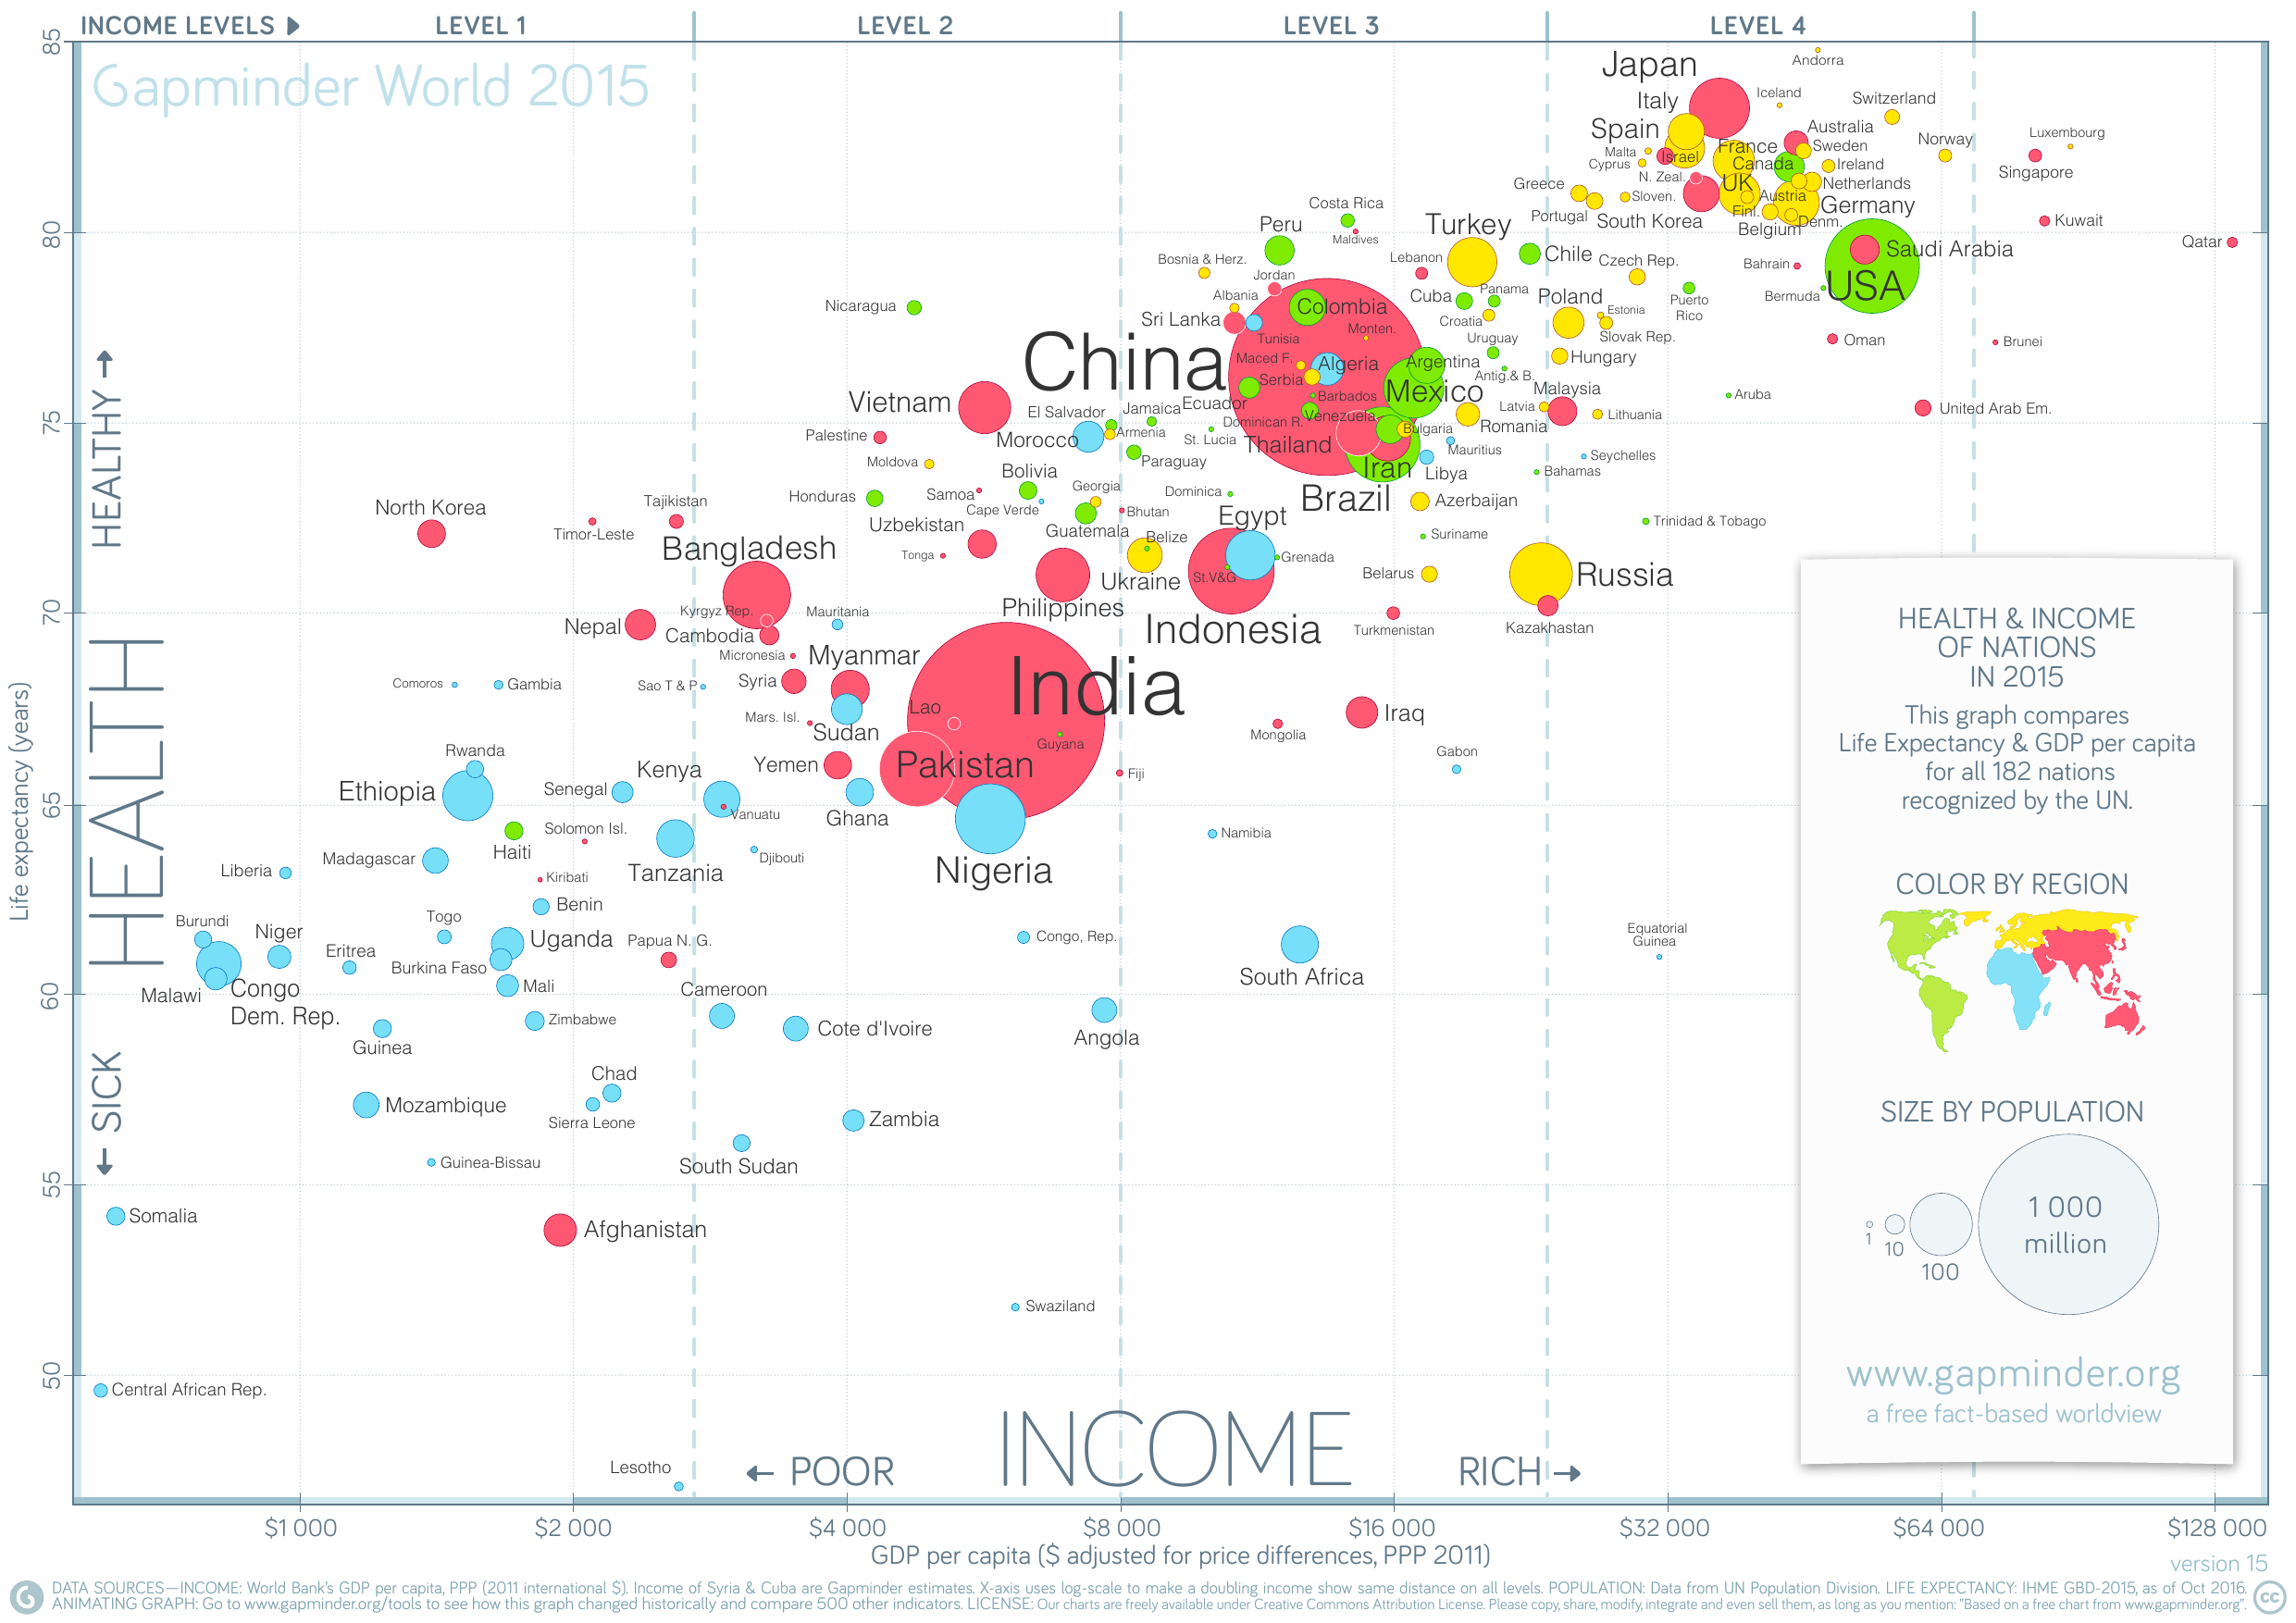
\includegraphics[width=1\linewidth]{images/countries-1} \end{center}

\begin{itemize}
\item
  O gráfico mostra como, em cada país, a saúde (mais precisamente, a expectativa de vida) se relaciona com a riqueza (mais precisamente, o PIB \emph{per capita}).
\item
  Além da expectativa de vida e o do PIB \emph{per capita}, o gráfico traz mais informações sobre cada país.
\item
  Cada país é representado por um ponto (a {\hl{geometria}}).
\item
  Informações sobre cada país são representadas por características do ponto correspondente (as {\hl{estéticas}}):

  \begin{longtable}[]{@{}lll@{}}
  \toprule
  Variável & Geometria & Estética \\
  \midrule
  \endhead
  PIB \emph{per capita} & ponto & posição x \\
  Expectativa de vida & ponto & posição y \\
  População & ponto & tamanho \\
  Continente & ponto & cor \\
  \bottomrule
  \end{longtable}
\item
  Você pode usar outras estéticas para representar informações:

  \begin{itemize}
  \tightlist
  \item
    Cor de preenchimento.
  \item
    Cor do traço.
  \item
    Tipo do traço (sólido, pontilhado, tracejado etc.).
  \item
    Forma (círculo, quadrado, triângulo etc.).
  \item
    Opacidade.
  \item
    etc.
  \end{itemize}
\item
  Você pode usar outras geometrias:

  \begin{itemize}
  \tightlist
  \item
    Linhas.
  \item
    Barras ou colunas.
  \item
    Caixas.
  \item
    etc.
  \end{itemize}
\end{itemize}

\hypertarget{escalas-scales}{%
\subsection{\texorpdfstring{Escalas (\emph{scales})}{Escalas (scales)}}\label{escalas-scales}}

\begin{itemize}
\item
  As escalas controlam os detalhes da aparência da geometria e do mapeamento (eixos, cores etc.).
\item
  Os eixos do gráfico acima são escalas {\hl{contínuas}}, com valores reais.
\item
  Observe o eixo horizontal. Os valores não aumentam linearmente, mas sim exponencialmente: cada passo à direita equivale a \emph{dobrar} o valor do PIB. O eixo horizontal segue uma {\hl{escala logarítmica}}.
\item
  Os tamanhos dos pontos formam uma escala {\hl{discreta}}, com $4$ valores possíveis (veja a legenda no canto inferior direito do gráfico).
\item
  As cores também formam uma escala discreta.
\end{itemize}

\hypertarget{ruxf3tulos-labels}{%
\subsection{\texorpdfstring{Rótulos (\emph{labels})}{Rótulos (labels)}}\label{ruxf3tulos-labels}}

\begin{itemize}
\item
  O gráfico também representa informação na forma de texto.
\item
  Além de rótulos (por exemplo, o texto que identifica cada eixo), {\hl{o texto também pode, ele mesmo, ser uma geometria, com suas próprias estéticas:}} observe como o nome de cada país é escrito em um tamanho proporcional à sua população.
\end{itemize}

\hypertarget{outros-componentes}{%
\subsection{Outros componentes}\label{outros-componentes}}

\begin{itemize}
\item
  Coordenadas:

  \begin{itemize}
  \item
    Este gráfico usa {\hl{coordenadas cartesianas}}, com eixos $x$ e $y$.
  \item
    Existem gráficos que usam um sistema de {\hl{coordenadas polares}}.
  \end{itemize}
\item
  Temas:

  \begin{itemize}
  \item
    Incluem todos os elementos ``decorativos'': cor de fundo, linhas de grade, etc. Ajudam a facilitar a leitura e a interpretação.
  \item
    No gráfico acima, um detalhe interessante do tema é a divisão de cada eixo em segmentos claros e segmentos escuros.
  \end{itemize}
\item
  Legendas (\emph{guides}).
\item
  Facetas:

  \begin{itemize}
  \item
    Às vezes, um gráfico é composto por múltiplos subgráficos.
  \item
    Cada subgráfico é uma {\hl{faceta}}.
  \item
    Facetas evitam que informações demais sejam apresentadas no mesmo lugar.
  \end{itemize}
\end{itemize}

\hypertarget{conjunto-de-dados}{%
\section{Conjunto de dados}\label{conjunto-de-dados}}

\begin{itemize}
\item
  Nossos exemplos de gráficos vão usar dados sobre o sono de diversos mamíferos.
\item
  O conjunto de dados se chama \texttt{msleep} e está incluído no pacote \texttt{ggplot2}.
\item
  Para ver a documentação, digite

\begin{Shaded}
\begin{Highlighting}[]
\FunctionTok{library}\NormalTok{(ggplot2)}
\NormalTok{?msleep}
\end{Highlighting}
\end{Shaded}
\item
  Vamos atribuir o conjunto de dados à variável \texttt{df}:

\begin{Shaded}
\begin{Highlighting}[]
\NormalTok{df }\OtherTok{\textless{}{-}}\NormalTok{ msleep}
\NormalTok{df}
\DocumentationTok{\#\# \# A tibble: 83 x 11}
\DocumentationTok{\#\#   name         genus   vore  order   conservation sleep\_total sleep\_rem}
\DocumentationTok{\#\#   \textless{}chr\textgreater{}        \textless{}chr\textgreater{}   \textless{}chr\textgreater{} \textless{}chr\textgreater{}   \textless{}chr\textgreater{}              \textless{}dbl\textgreater{}     \textless{}dbl\textgreater{}}
\DocumentationTok{\#\# 1 Cheetah      Acinon\textasciitilde{} carni Carniv\textasciitilde{} lc                  12.1      NA  }
\DocumentationTok{\#\# 2 Owl monkey   Aotus   omni  Primat\textasciitilde{} \textless{}NA\textgreater{}                17         1.8}
\DocumentationTok{\#\# 3 Mountain be\textasciitilde{} Aplodo\textasciitilde{} herbi Rodent\textasciitilde{} nt                  14.4       2.4}
\DocumentationTok{\#\# 4 Greater sho\textasciitilde{} Blarina omni  Sorico\textasciitilde{} lc                  14.9       2.3}
\DocumentationTok{\#\# 5 Cow          Bos     herbi Artiod\textasciitilde{} domesticated         4         0.7}
\DocumentationTok{\#\# 6 Three{-}toed \textasciitilde{} Bradyp\textasciitilde{} herbi Pilosa  \textless{}NA\textgreater{}                14.4       2.2}
\DocumentationTok{\#\# \# ... with 77 more rows, and 4 more variables: sleep\_cycle \textless{}dbl\textgreater{},}
\DocumentationTok{\#\# \#   awake \textless{}dbl\textgreater{}, brainwt \textless{}dbl\textgreater{}, bodywt \textless{}dbl\textgreater{}}
\end{Highlighting}
\end{Shaded}
\item
  Vamos examinar a estrutura --- usando R base:

\begin{Shaded}
\begin{Highlighting}[]
\FunctionTok{str}\NormalTok{(df)}
\DocumentationTok{\#\# tibble [83 x 11] (S3: tbl\_df/tbl/data.frame)}
\DocumentationTok{\#\#  $ name        : chr [1:83] "Cheetah" "Owl monkey" "Mountain beaver" ...}
\DocumentationTok{\#\#  $ genus       : chr [1:83] "Acinonyx" "Aotus" "Aplodontia" ...}
\DocumentationTok{\#\#  $ vore        : chr [1:83] "carni" "omni" "herbi" ...}
\DocumentationTok{\#\#  $ order       : chr [1:83] "Carnivora" "Primates" "Rodentia" ...}
\DocumentationTok{\#\#  $ conservation: chr [1:83] "lc" NA "nt" ...}
\DocumentationTok{\#\#  $ sleep\_total : num [1:83] 12,1 17 14,4 14,9 4 14,4 8,7 7 ...}
\DocumentationTok{\#\#  $ sleep\_rem   : num [1:83] NA 1,8 2,4 2,3 0,7 2,2 1,4 NA ...}
\DocumentationTok{\#\#  $ sleep\_cycle : num [1:83] NA NA NA 0,133 ...}
\DocumentationTok{\#\#  $ awake       : num [1:83] 11,9 7 9,6 9,1 20 9,6 15,3 17 ...}
\DocumentationTok{\#\#  $ brainwt     : num [1:83] NA 0,0155 NA 0,00029 0,423 NA NA NA ...}
\DocumentationTok{\#\#  $ bodywt      : num [1:83] 50 0,48 1,35 0,019 ...}
\end{Highlighting}
\end{Shaded}
\item
  Podemos usar \texttt{glimpse}, uma função do \texttt{tidyverse}:

\begin{Shaded}
\begin{Highlighting}[]
\FunctionTok{glimpse}\NormalTok{(df)}
\DocumentationTok{\#\# Rows: 83}
\DocumentationTok{\#\# Columns: 11}
\DocumentationTok{\#\# $ name         \textless{}chr\textgreater{} "Cheetah", "Owl monkey", "Mountain beaver", "Gre\textasciitilde{}}
\DocumentationTok{\#\# $ genus        \textless{}chr\textgreater{} "Acinonyx", "Aotus", "Aplodontia", "Blarina", "B\textasciitilde{}}
\DocumentationTok{\#\# $ vore         \textless{}chr\textgreater{} "carni", "omni", "herbi", "omni", "herbi", "herb\textasciitilde{}}
\DocumentationTok{\#\# $ order        \textless{}chr\textgreater{} "Carnivora", "Primates", "Rodentia", "Soricomorp\textasciitilde{}}
\DocumentationTok{\#\# $ conservation \textless{}chr\textgreater{} "lc", NA, "nt", "lc", "domesticated", NA, "vu", \textasciitilde{}}
\DocumentationTok{\#\# $ sleep\_total  \textless{}dbl\textgreater{} 12,1, 17,0, 14,4, 14,9, 4,0, 14,4, 8,7, 7,0, 10,\textasciitilde{}}
\DocumentationTok{\#\# $ sleep\_rem    \textless{}dbl\textgreater{} NA, 1,8, 2,4, 2,3, 0,7, 2,2, 1,4, NA, 2,9, NA, 0\textasciitilde{}}
\DocumentationTok{\#\# $ sleep\_cycle  \textless{}dbl\textgreater{} NA, NA, NA, 0,1333333, 0,6666667, 0,7666667, 0,3\textasciitilde{}}
\DocumentationTok{\#\# $ awake        \textless{}dbl\textgreater{} 11,9, 7,0, 9,6, 9,1, 20,0, 9,6, 15,3, 17,0, 13,9\textasciitilde{}}
\DocumentationTok{\#\# $ brainwt      \textless{}dbl\textgreater{} NA, 0,01550, NA, 0,00029, 0,42300, NA, NA, NA, 0\textasciitilde{}}
\DocumentationTok{\#\# $ bodywt       \textless{}dbl\textgreater{} 50,000, 0,480, 1,350, 0,019, 600,000, 3,850, 20,\textasciitilde{}}
\end{Highlighting}
\end{Shaded}
\item
  Para examinar só as primeiras linhas do \emph{data frame}:

\begin{Shaded}
\begin{Highlighting}[]
\FunctionTok{head}\NormalTok{(df)}
\DocumentationTok{\#\# \# A tibble: 6 x 11}
\DocumentationTok{\#\#   name         genus   vore  order   conservation sleep\_total sleep\_rem}
\DocumentationTok{\#\#   \textless{}chr\textgreater{}        \textless{}chr\textgreater{}   \textless{}chr\textgreater{} \textless{}chr\textgreater{}   \textless{}chr\textgreater{}              \textless{}dbl\textgreater{}     \textless{}dbl\textgreater{}}
\DocumentationTok{\#\# 1 Cheetah      Acinon\textasciitilde{} carni Carniv\textasciitilde{} lc                  12.1      NA  }
\DocumentationTok{\#\# 2 Owl monkey   Aotus   omni  Primat\textasciitilde{} \textless{}NA\textgreater{}                17         1.8}
\DocumentationTok{\#\# 3 Mountain be\textasciitilde{} Aplodo\textasciitilde{} herbi Rodent\textasciitilde{} nt                  14.4       2.4}
\DocumentationTok{\#\# 4 Greater sho\textasciitilde{} Blarina omni  Sorico\textasciitilde{} lc                  14.9       2.3}
\DocumentationTok{\#\# 5 Cow          Bos     herbi Artiod\textasciitilde{} domesticated         4         0.7}
\DocumentationTok{\#\# 6 Three{-}toed \textasciitilde{} Bradyp\textasciitilde{} herbi Pilosa  \textless{}NA\textgreater{}                14.4       2.2}
\DocumentationTok{\#\# \# ... with 4 more variables: sleep\_cycle \textless{}dbl\textgreater{}, awake \textless{}dbl\textgreater{},}
\DocumentationTok{\#\# \#   brainwt \textless{}dbl\textgreater{}, bodywt \textless{}dbl\textgreater{}}
\end{Highlighting}
\end{Shaded}
\item
  Para examinar o \emph{data frame} interativamente:

\begin{Shaded}
\begin{Highlighting}[]
\FunctionTok{view}\NormalTok{(df)}
\end{Highlighting}
\end{Shaded}
\item
  Podemos produzir um sumário dos dados usando o pacote \emph{summarytools} (que já foi carregado neste documento):

\begin{Shaded}
\begin{Highlighting}[]
\NormalTok{df }\SpecialCharTok{\%\textgreater{}\%} \FunctionTok{dfSummary}\NormalTok{() }\SpecialCharTok{\%\textgreater{}\%} \FunctionTok{print}\NormalTok{()}
\end{Highlighting}
\end{Shaded}

  \begin{longtable}[]{@{}
    >{\raggedright\arraybackslash}p{(\columnwidth - 6\tabcolsep) * \real{0.1928}}
    >{\raggedright\arraybackslash}p{(\columnwidth - 6\tabcolsep) * \real{0.3976}}
    >{\raggedright\arraybackslash}p{(\columnwidth - 6\tabcolsep) * \real{0.2771}}
    >{\raggedright\arraybackslash}p{(\columnwidth - 6\tabcolsep) * \real{0.1325}}@{}}
  \toprule
  \begin{minipage}[b]{\linewidth}\raggedright
  Variável
  \end{minipage} & \begin{minipage}[b]{\linewidth}\raggedright
  Estatísticas / Valores
  \end{minipage} & \begin{minipage}[b]{\linewidth}\raggedright
  Freqs (\% de Válidos)
  \end{minipage} & \begin{minipage}[b]{\linewidth}\raggedright
  Faltante
  \end{minipage} \\
  \midrule
  \endhead
  \begin{minipage}[t]{\linewidth}\raggedright
  name\\
  {[}character{]}\strut
  \end{minipage} & \begin{minipage}[t]{\linewidth}\raggedright
  1. African elephant\\
  2. African giant pouched rat\\
  3. African striped mouse\\
  4. Arctic fox\\
  5. Arctic ground squirrel\\
  6. Asian elephant\\
  7. Baboon\\
  8. Big brown bat\\
  9. Bottle-nosed dolphin\\
  10. Brazilian tapir\\
  {[} 73 outros {]}\strut
  \end{minipage} & \begin{minipage}[t]{\linewidth}\raggedright
  1 ( 1,2\%)\\
  1 ( 1,2\%)\\
  1 ( 1,2\%)\\
  1 ( 1,2\%)\\
  1 ( 1,2\%)\\
  1 ( 1,2\%)\\
  1 ( 1,2\%)\\
  1 ( 1,2\%)\\
  1 ( 1,2\%)\\
  1 ( 1,2\%)\\
  73 (88,0\%)\strut
  \end{minipage} & \begin{minipage}[t]{\linewidth}\raggedright
  0\\
  (0,0\%)\strut
  \end{minipage} \\
  \begin{minipage}[t]{\linewidth}\raggedright
  genus\\
  {[}character{]}\strut
  \end{minipage} & \begin{minipage}[t]{\linewidth}\raggedright
  1. Panthera\\
  2. Spermophilus\\
  3. Equus\\
  4. Vulpes\\
  5. Acinonyx\\
  6. Aotus\\
  7. Aplodontia\\
  8. Blarina\\
  9. Bos\\
  10. Bradypus\\
  {[} 67 outros {]}\strut
  \end{minipage} & \begin{minipage}[t]{\linewidth}\raggedright
  3 ( 3,6\%)\\
  3 ( 3,6\%)\\
  2 ( 2,4\%)\\
  2 ( 2,4\%)\\
  1 ( 1,2\%)\\
  1 ( 1,2\%)\\
  1 ( 1,2\%)\\
  1 ( 1,2\%)\\
  1 ( 1,2\%)\\
  1 ( 1,2\%)\\
  67 (80,7\%)\strut
  \end{minipage} & \begin{minipage}[t]{\linewidth}\raggedright
  0\\
  (0,0\%)\strut
  \end{minipage} \\
  \begin{minipage}[t]{\linewidth}\raggedright
  vore\\
  {[}character{]}\strut
  \end{minipage} & \begin{minipage}[t]{\linewidth}\raggedright
  1. carni\\
  2. herbi\\
  3. insecti\\
  4. omni\strut
  \end{minipage} & \begin{minipage}[t]{\linewidth}\raggedright
  19 (25,0\%)\\
  32 (42,1\%)\\
  5 ( 6,6\%)\\
  20 (26,3\%)\strut
  \end{minipage} & \begin{minipage}[t]{\linewidth}\raggedright
  7\\
  (8,4\%)\strut
  \end{minipage} \\
  \begin{minipage}[t]{\linewidth}\raggedright
  order\\
  {[}character{]}\strut
  \end{minipage} & \begin{minipage}[t]{\linewidth}\raggedright
  1. Rodentia\\
  2. Carnivora\\
  3. Primates\\
  4. Artiodactyla\\
  5. Soricomorpha\\
  6. Cetacea\\
  7. Hyracoidea\\
  8. Perissodactyla\\
  9. Chiroptera\\
  10. Cingulata\\
  {[} 9 outros {]}\strut
  \end{minipage} & \begin{minipage}[t]{\linewidth}\raggedright
  22 (26,5\%)\\
  12 (14,5\%)\\
  12 (14,5\%)\\
  6 ( 7,2\%)\\
  5 ( 6,0\%)\\
  3 ( 3,6\%)\\
  3 ( 3,6\%)\\
  3 ( 3,6\%)\\
  2 ( 2,4\%)\\
  2 ( 2,4\%)\\
  13 (15,7\%)\strut
  \end{minipage} & \begin{minipage}[t]{\linewidth}\raggedright
  0\\
  (0,0\%)\strut
  \end{minipage} \\
  \begin{minipage}[t]{\linewidth}\raggedright
  conservation\\
  {[}character{]}\strut
  \end{minipage} & \begin{minipage}[t]{\linewidth}\raggedright
  1. cd\\
  2. domesticated\\
  3. en\\
  4. lc\\
  5. nt\\
  6. vu\strut
  \end{minipage} & \begin{minipage}[t]{\linewidth}\raggedright
  2 ( 3,7\%)\\
  10 (18,5\%)\\
  4 ( 7,4\%)\\
  27 (50,0\%)\\
  4 ( 7,4\%)\\
  7 (13,0\%)\strut
  \end{minipage} & \begin{minipage}[t]{\linewidth}\raggedright
  29\\
  (34,9\%)\strut
  \end{minipage} \\
  \begin{minipage}[t]{\linewidth}\raggedright
  sleep\_total\\
  {[}numeric{]}\strut
  \end{minipage} & \begin{minipage}[t]{\linewidth}\raggedright
  Média (dp) : 10,4 (4,5)\\
  mín \textless{} mediana \textless{} máx:\\
  1,9 \textless{} 10,1 \textless{} 19,9\\
  IQE (CV) : 5,9 (0,4)\strut
  \end{minipage} & 65 valores distintos & \begin{minipage}[t]{\linewidth}\raggedright
  0\\
  (0,0\%)\strut
  \end{minipage} \\
  \begin{minipage}[t]{\linewidth}\raggedright
  sleep\_rem\\
  {[}numeric{]}\strut
  \end{minipage} & \begin{minipage}[t]{\linewidth}\raggedright
  Média (dp) : 1,9 (1,3)\\
  mín \textless{} mediana \textless{} máx:\\
  0,1 \textless{} 1,5 \textless{} 6,6\\
  IQE (CV) : 1,5 (0,7)\strut
  \end{minipage} & 32 valores distintos & \begin{minipage}[t]{\linewidth}\raggedright
  22\\
  (26,5\%)\strut
  \end{minipage} \\
  \begin{minipage}[t]{\linewidth}\raggedright
  sleep\_cycle\\
  {[}numeric{]}\strut
  \end{minipage} & \begin{minipage}[t]{\linewidth}\raggedright
  Média (dp) : 0,4 (0,4)\\
  mín \textless{} mediana \textless{} máx:\\
  0,1 \textless{} 0,3 \textless{} 1,5\\
  IQE (CV) : 0,4 (0,8)\strut
  \end{minipage} & 22 valores distintos & \begin{minipage}[t]{\linewidth}\raggedright
  51\\
  (61,4\%)\strut
  \end{minipage} \\
  \begin{minipage}[t]{\linewidth}\raggedright
  awake\\
  {[}numeric{]}\strut
  \end{minipage} & \begin{minipage}[t]{\linewidth}\raggedright
  Média (dp) : 13,6 (4,5)\\
  mín \textless{} mediana \textless{} máx:\\
  4,1 \textless{} 13,9 \textless{} 22,1\\
  IQE (CV) : 5,9 (0,3)\strut
  \end{minipage} & 65 valores distintos & \begin{minipage}[t]{\linewidth}\raggedright
  0\\
  (0,0\%)\strut
  \end{minipage} \\
  \begin{minipage}[t]{\linewidth}\raggedright
  brainwt\\
  {[}numeric{]}\strut
  \end{minipage} & \begin{minipage}[t]{\linewidth}\raggedright
  Média (dp) : 0,3 (1)\\
  mín \textless{} mediana \textless{} máx:\\
  0 \textless{} 0 \textless{} 5,7\\
  IQE (CV) : 0,1 (3,5)\strut
  \end{minipage} & 53 valores distintos & \begin{minipage}[t]{\linewidth}\raggedright
  27\\
  (32,5\%)\strut
  \end{minipage} \\
  \begin{minipage}[t]{\linewidth}\raggedright
  bodywt\\
  {[}numeric{]}\strut
  \end{minipage} & \begin{minipage}[t]{\linewidth}\raggedright
  Média (dp) : 166,1 (786,8)\\
  mín \textless{} mediana \textless{} máx:\\
  0 \textless{} 1,7 \textless{} 6654\\
  IQE (CV) : 41,6 (4,7)\strut
  \end{minipage} & 82 valores distintos & \begin{minipage}[t]{\linewidth}\raggedright
  0\\
  (0,0\%)\strut
  \end{minipage} \\
  \bottomrule
  \end{longtable}
\item
  Vemos que há muitos \texttt{NA} em diversas variáveis. Para nossos exemplos simples de visualização, vamos usar as colunas

  \begin{itemize}
  \tightlist
  \item
    \texttt{name}
  \item
    \texttt{genus}
  \item
    \texttt{order}
  \item
    \texttt{sleep\_total}
  \item
    \texttt{awake}
  \item
    \texttt{bodywt}
  \item
    \texttt{brainwt}
  \end{itemize}
\item
  Mas\ldots{} a coluna que mostra a dieta (\texttt{vore}) tem só 7 \texttt{NA}. Quais são?

\begin{Shaded}
\begin{Highlighting}[]
\NormalTok{df }\SpecialCharTok{\%\textgreater{}\%} 
  \FunctionTok{filter}\NormalTok{(}\FunctionTok{is.na}\NormalTok{(vore)) }\SpecialCharTok{\%\textgreater{}\%} 
  \FunctionTok{select}\NormalTok{(name)}
\DocumentationTok{\#\# \# A tibble: 7 x 1}
\DocumentationTok{\#\#   name           }
\DocumentationTok{\#\#   \textless{}chr\textgreater{}          }
\DocumentationTok{\#\# 1 Vesper mouse   }
\DocumentationTok{\#\# 2 Desert hedgehog}
\DocumentationTok{\#\# 3 Deer mouse     }
\DocumentationTok{\#\# 4 Phalanger      }
\DocumentationTok{\#\# 5 Rock hyrax     }
\DocumentationTok{\#\# 6 Mole rat       }
\DocumentationTok{\#\# \# ... with 1 more row}
\end{Highlighting}
\end{Shaded}
\item
  OK. Vamos manter a coluna \texttt{vore} também, apesar dos \texttt{NA}. Quando formos usar esta variável, tomaremos cuidado.
\item
  Também\ldots{} a coluna \texttt{bodywt} tem 0 como valor mínimo. Como assim?

\begin{Shaded}
\begin{Highlighting}[]
\NormalTok{df }\SpecialCharTok{\%\textgreater{}\%} 
  \FunctionTok{filter}\NormalTok{(bodywt }\SpecialCharTok{\textless{}} \DecValTok{1}\NormalTok{) }\SpecialCharTok{\%\textgreater{}\%} 
  \FunctionTok{select}\NormalTok{(name, bodywt) }\SpecialCharTok{\%\textgreater{}\%} 
  \FunctionTok{arrange}\NormalTok{(bodywt)}
\DocumentationTok{\#\# \# A tibble: 35 x 2}
\DocumentationTok{\#\#   name                       bodywt}
\DocumentationTok{\#\#   \textless{}chr\textgreater{}                       \textless{}dbl\textgreater{}}
\DocumentationTok{\#\# 1 Lesser short{-}tailed shrew   0.005}
\DocumentationTok{\#\# 2 Little brown bat            0.01 }
\DocumentationTok{\#\# 3 Greater short{-}tailed shrew  0.019}
\DocumentationTok{\#\# 4 Deer mouse                  0.021}
\DocumentationTok{\#\# 5 House mouse                 0.022}
\DocumentationTok{\#\# 6 Big brown bat               0.023}
\DocumentationTok{\#\# \# ... with 29 more rows}
\end{Highlighting}
\end{Shaded}
\item
  Ah, sem problema. A função \texttt{dfSummary} arredondou estes pesos para 0. Os valores de verdade ainda estão na \emph{tibble}.
\item
  Vamos criar uma \emph{tibble} nova, só com as colunas que nos interessam:

\begin{Shaded}
\begin{Highlighting}[]
\NormalTok{sono }\OtherTok{\textless{}{-}}\NormalTok{ df }\SpecialCharTok{\%\textgreater{}\%} 
  \FunctionTok{select}\NormalTok{(}
\NormalTok{    name, order, genus, vore, bodywt, }
\NormalTok{    brainwt, awake, sleep\_total}
\NormalTok{  )}
\end{Highlighting}
\end{Shaded}
\item
  Vamos ver o sumário:

\begin{Shaded}
\begin{Highlighting}[]
\NormalTok{sono }\SpecialCharTok{\%\textgreater{}\%} \FunctionTok{dfSummary}\NormalTok{() }\SpecialCharTok{\%\textgreater{}\%} \FunctionTok{print}\NormalTok{()}
\end{Highlighting}
\end{Shaded}

  \begin{longtable}[]{@{}
    >{\raggedright\arraybackslash}p{(\columnwidth - 6\tabcolsep) * \real{0.1829}}
    >{\raggedright\arraybackslash}p{(\columnwidth - 6\tabcolsep) * \real{0.4024}}
    >{\raggedright\arraybackslash}p{(\columnwidth - 6\tabcolsep) * \real{0.2805}}
    >{\raggedright\arraybackslash}p{(\columnwidth - 6\tabcolsep) * \real{0.1341}}@{}}
  \toprule
  \begin{minipage}[b]{\linewidth}\raggedright
  Variável
  \end{minipage} & \begin{minipage}[b]{\linewidth}\raggedright
  Estatísticas / Valores
  \end{minipage} & \begin{minipage}[b]{\linewidth}\raggedright
  Freqs (\% de Válidos)
  \end{minipage} & \begin{minipage}[b]{\linewidth}\raggedright
  Faltante
  \end{minipage} \\
  \midrule
  \endhead
  \begin{minipage}[t]{\linewidth}\raggedright
  name\\
  {[}character{]}\strut
  \end{minipage} & \begin{minipage}[t]{\linewidth}\raggedright
  1. African elephant\\
  2. African giant pouched rat\\
  3. African striped mouse\\
  4. Arctic fox\\
  5. Arctic ground squirrel\\
  6. Asian elephant\\
  7. Baboon\\
  8. Big brown bat\\
  9. Bottle-nosed dolphin\\
  10. Brazilian tapir\\
  {[} 73 outros {]}\strut
  \end{minipage} & \begin{minipage}[t]{\linewidth}\raggedright
  1 ( 1,2\%)\\
  1 ( 1,2\%)\\
  1 ( 1,2\%)\\
  1 ( 1,2\%)\\
  1 ( 1,2\%)\\
  1 ( 1,2\%)\\
  1 ( 1,2\%)\\
  1 ( 1,2\%)\\
  1 ( 1,2\%)\\
  1 ( 1,2\%)\\
  73 (88,0\%)\strut
  \end{minipage} & \begin{minipage}[t]{\linewidth}\raggedright
  0\\
  (0,0\%)\strut
  \end{minipage} \\
  \begin{minipage}[t]{\linewidth}\raggedright
  order\\
  {[}character{]}\strut
  \end{minipage} & \begin{minipage}[t]{\linewidth}\raggedright
  1. Rodentia\\
  2. Carnivora\\
  3. Primates\\
  4. Artiodactyla\\
  5. Soricomorpha\\
  6. Cetacea\\
  7. Hyracoidea\\
  8. Perissodactyla\\
  9. Chiroptera\\
  10. Cingulata\\
  {[} 9 outros {]}\strut
  \end{minipage} & \begin{minipage}[t]{\linewidth}\raggedright
  22 (26,5\%)\\
  12 (14,5\%)\\
  12 (14,5\%)\\
  6 ( 7,2\%)\\
  5 ( 6,0\%)\\
  3 ( 3,6\%)\\
  3 ( 3,6\%)\\
  3 ( 3,6\%)\\
  2 ( 2,4\%)\\
  2 ( 2,4\%)\\
  13 (15,7\%)\strut
  \end{minipage} & \begin{minipage}[t]{\linewidth}\raggedright
  0\\
  (0,0\%)\strut
  \end{minipage} \\
  \begin{minipage}[t]{\linewidth}\raggedright
  genus\\
  {[}character{]}\strut
  \end{minipage} & \begin{minipage}[t]{\linewidth}\raggedright
  1. Panthera\\
  2. Spermophilus\\
  3. Equus\\
  4. Vulpes\\
  5. Acinonyx\\
  6. Aotus\\
  7. Aplodontia\\
  8. Blarina\\
  9. Bos\\
  10. Bradypus\\
  {[} 67 outros {]}\strut
  \end{minipage} & \begin{minipage}[t]{\linewidth}\raggedright
  3 ( 3,6\%)\\
  3 ( 3,6\%)\\
  2 ( 2,4\%)\\
  2 ( 2,4\%)\\
  1 ( 1,2\%)\\
  1 ( 1,2\%)\\
  1 ( 1,2\%)\\
  1 ( 1,2\%)\\
  1 ( 1,2\%)\\
  1 ( 1,2\%)\\
  67 (80,7\%)\strut
  \end{minipage} & \begin{minipage}[t]{\linewidth}\raggedright
  0\\
  (0,0\%)\strut
  \end{minipage} \\
  \begin{minipage}[t]{\linewidth}\raggedright
  vore\\
  {[}character{]}\strut
  \end{minipage} & \begin{minipage}[t]{\linewidth}\raggedright
  1. carni\\
  2. herbi\\
  3. insecti\\
  4. omni\strut
  \end{minipage} & \begin{minipage}[t]{\linewidth}\raggedright
  19 (25,0\%)\\
  32 (42,1\%)\\
  5 ( 6,6\%)\\
  20 (26,3\%)\strut
  \end{minipage} & \begin{minipage}[t]{\linewidth}\raggedright
  7\\
  (8,4\%)\strut
  \end{minipage} \\
  \begin{minipage}[t]{\linewidth}\raggedright
  bodywt\\
  {[}numeric{]}\strut
  \end{minipage} & \begin{minipage}[t]{\linewidth}\raggedright
  Média (dp) : 166,1 (786,8)\\
  mín \textless{} mediana \textless{} máx:\\
  0 \textless{} 1,7 \textless{} 6654\\
  IQE (CV) : 41,6 (4,7)\strut
  \end{minipage} & 82 valores distintos & \begin{minipage}[t]{\linewidth}\raggedright
  0\\
  (0,0\%)\strut
  \end{minipage} \\
  \begin{minipage}[t]{\linewidth}\raggedright
  brainwt\\
  {[}numeric{]}\strut
  \end{minipage} & \begin{minipage}[t]{\linewidth}\raggedright
  Média (dp) : 0,3 (1)\\
  mín \textless{} mediana \textless{} máx:\\
  0 \textless{} 0 \textless{} 5,7\\
  IQE (CV) : 0,1 (3,5)\strut
  \end{minipage} & 53 valores distintos & \begin{minipage}[t]{\linewidth}\raggedright
  27\\
  (32,5\%)\strut
  \end{minipage} \\
  \begin{minipage}[t]{\linewidth}\raggedright
  awake\\
  {[}numeric{]}\strut
  \end{minipage} & \begin{minipage}[t]{\linewidth}\raggedright
  Média (dp) : 13,6 (4,5)\\
  mín \textless{} mediana \textless{} máx:\\
  4,1 \textless{} 13,9 \textless{} 22,1\\
  IQE (CV) : 5,9 (0,3)\strut
  \end{minipage} & 65 valores distintos & \begin{minipage}[t]{\linewidth}\raggedright
  0\\
  (0,0\%)\strut
  \end{minipage} \\
  \begin{minipage}[t]{\linewidth}\raggedright
  sleep\_total\\
  {[}numeric{]}\strut
  \end{minipage} & \begin{minipage}[t]{\linewidth}\raggedright
  Média (dp) : 10,4 (4,5)\\
  mín \textless{} mediana \textless{} máx:\\
  1,9 \textless{} 10,1 \textless{} 19,9\\
  IQE (CV) : 5,9 (0,4)\strut
  \end{minipage} & 65 valores distintos & \begin{minipage}[t]{\linewidth}\raggedright
  0\\
  (0,0\%)\strut
  \end{minipage} \\
  \bottomrule
  \end{longtable}
\end{itemize}

\hypertarget{gruxe1ficos-de-dispersuxe3o-scatter-plots}{%
\section{\texorpdfstring{Gráficos de dispersão (\emph{scatter plots})}{Gráficos de dispersão (scatter plots)}}\label{gruxe1ficos-de-dispersuxe3o-scatter-plots}}

\begin{itemize}
\item
  Servem para visualizar a \emph{relação} entre {\hl{duas variáveis quantitativas.}}
\item
  {\hl{Essa relação \emph{não} é necessariamente de causa e efeito.}}
\item
  Isto é, a variável do eixo horizontal não determina, necessariamente, os valores da variável do eixo vertical.
\item
  Pense em {\hl{associação}}, {\hl{correlação}}, não em causalidade.
\item
  Troque as variáveis de eixo, se ajudar a deixar isto claro.
\end{itemize}

\hypertarget{horas-de-sono-e-peso-corporal}{%
\subsection{Horas de sono e peso corporal}\label{horas-de-sono-e-peso-corporal}}

\begin{itemize}
\item
  Como as variáveis \texttt{sleep\_total} e \texttt{bodywt} estão relacionadas?

\begin{Shaded}
\begin{Highlighting}[]
\NormalTok{sono }\SpecialCharTok{\%\textgreater{}\%} 
  \FunctionTok{ggplot}\NormalTok{(}\FunctionTok{aes}\NormalTok{(}\AttributeTok{x =}\NormalTok{ bodywt, }\AttributeTok{y =}\NormalTok{ sleep\_total))}
\end{Highlighting}
\end{Shaded}

  \begin{center}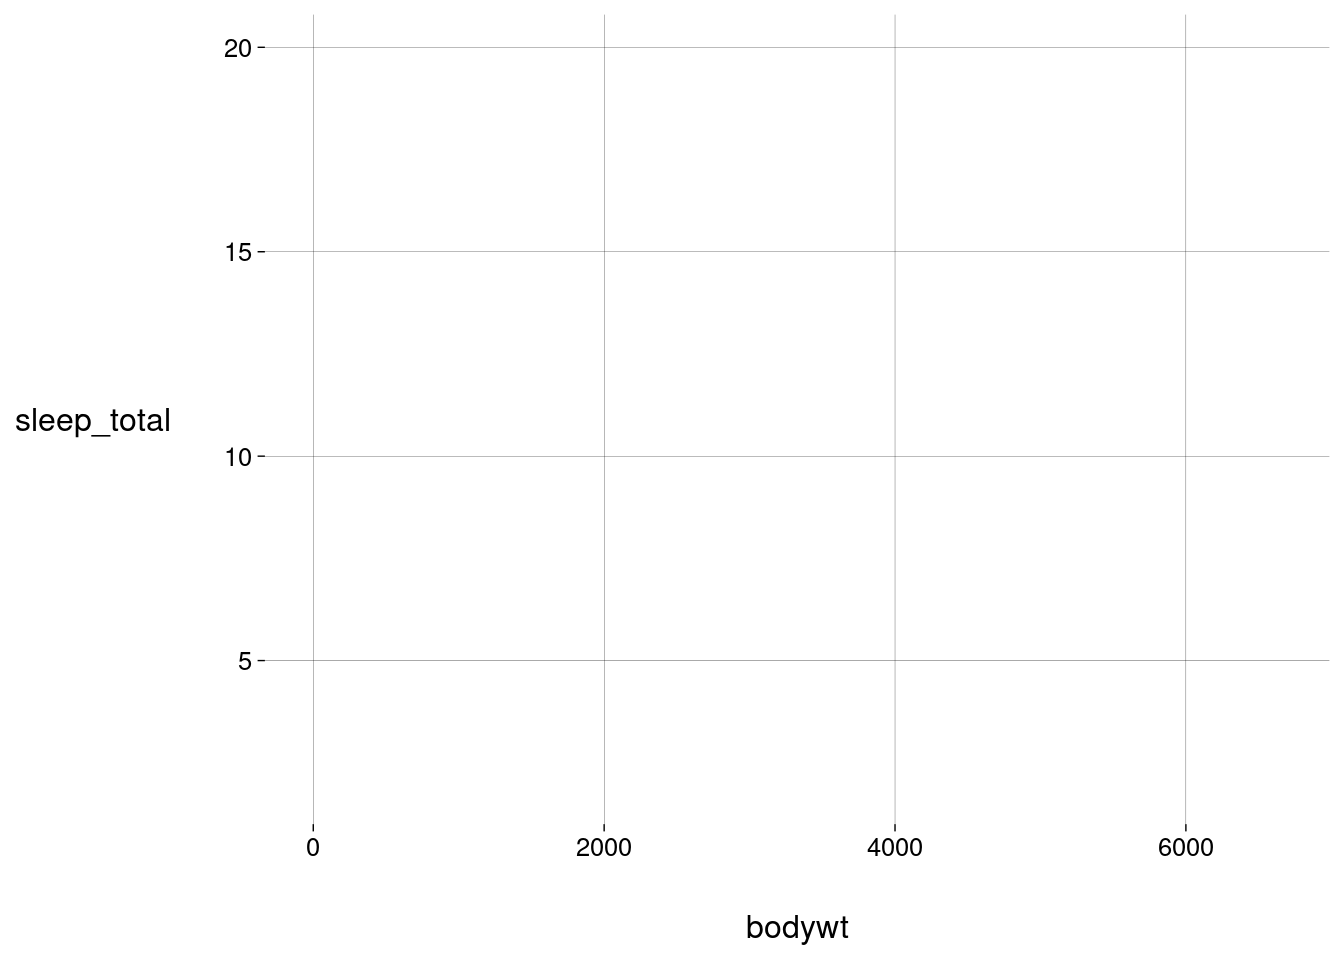
\includegraphics[width=1\linewidth]{_main_files/figure-latex/sono-peso-plot-1-1} \end{center}
\item
  O que houve? Cadê os pontos?
\item
  O problema foi que só especificamos o mapeamento estético (com \texttt{aes}, que são as iniciais de \emph{aesthetics}). {\hl{Faltou a geometria.}}

\begin{Shaded}
\begin{Highlighting}[]
\NormalTok{sono }\SpecialCharTok{\%\textgreater{}\%} 
  \FunctionTok{ggplot}\NormalTok{(}\FunctionTok{aes}\NormalTok{(}\AttributeTok{x =}\NormalTok{ bodywt, }\AttributeTok{y =}\NormalTok{ sleep\_total)) }\SpecialCharTok{+}
  \FunctionTok{geom\_point}\NormalTok{()}
\end{Highlighting}
\end{Shaded}

  \begin{center}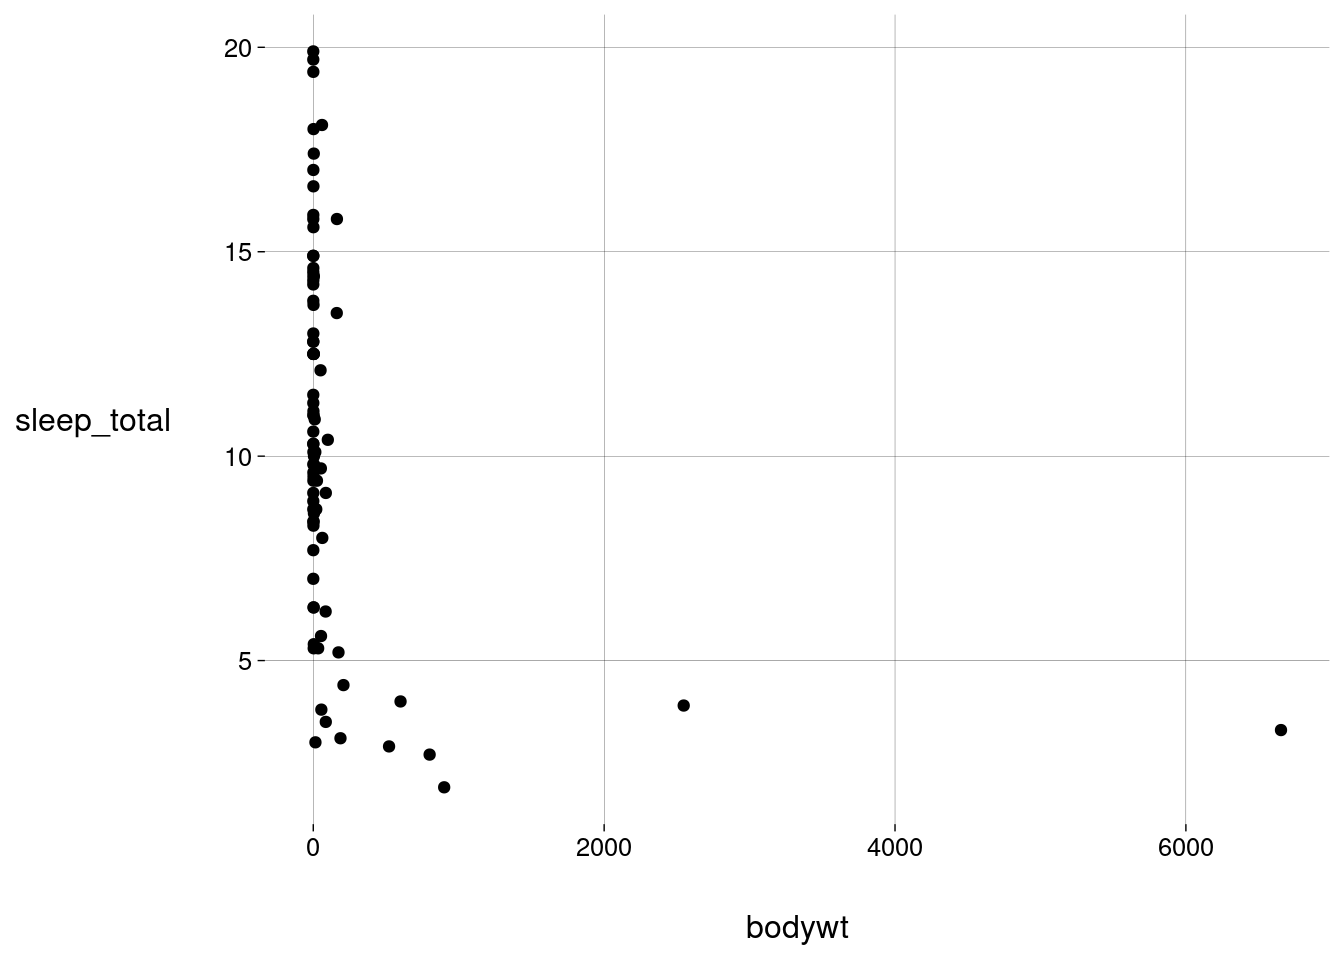
\includegraphics[width=1\linewidth]{_main_files/figure-latex/sono-peso-plot-2-1} \end{center}
\item
  Que horror.
\item
  A única coisa que percebemos aqui é que os mamíferos muito pesados dormem menos de $5$ horas por noite.
\item
  Estes animais muito pesados estão estragando a escala do eixo $x$.
\item
  Que animais são estes?

\begin{Shaded}
\begin{Highlighting}[]
\NormalTok{sono }\SpecialCharTok{\%\textgreater{}\%} 
  \FunctionTok{filter}\NormalTok{(bodywt }\SpecialCharTok{\textgreater{}} \DecValTok{250}\NormalTok{) }\SpecialCharTok{\%\textgreater{}\%} 
  \FunctionTok{select}\NormalTok{(name, bodywt) }\SpecialCharTok{\%\textgreater{}\%} 
  \FunctionTok{arrange}\NormalTok{(bodywt)}
\DocumentationTok{\#\# \# A tibble: 6 x 2}
\DocumentationTok{\#\#   name             bodywt}
\DocumentationTok{\#\#   \textless{}chr\textgreater{}             \textless{}dbl\textgreater{}}
\DocumentationTok{\#\# 1 Horse              521 }
\DocumentationTok{\#\# 2 Cow                600 }
\DocumentationTok{\#\# 3 Pilot whale        800 }
\DocumentationTok{\#\# 4 Giraffe            900.}
\DocumentationTok{\#\# 5 Asian elephant    2547 }
\DocumentationTok{\#\# 6 African elephant  6654}
\end{Highlighting}
\end{Shaded}
\item
  Além disso, há muitos pontos sobrepostos. Em bom português, temos um problema de \emph{overplotting}.
\item
  Existem diversas maneiras de lidar com isso.
\item
  A primeira delas é {\hl{alterando a opacidade dos pontos}}. Isto é um ajuste na geometria apenas, pois a opacidade, aqui, não representa informação nenhuma.

\begin{Shaded}
\begin{Highlighting}[]
\NormalTok{sono }\SpecialCharTok{\%\textgreater{}\%} 
  \FunctionTok{ggplot}\NormalTok{(}\FunctionTok{aes}\NormalTok{(}\AttributeTok{x =}\NormalTok{ bodywt, }\AttributeTok{y =}\NormalTok{ sleep\_total)) }\SpecialCharTok{+}
    \FunctionTok{geom\_point}\NormalTok{(}\AttributeTok{alpha =} \FloatTok{0.2}\NormalTok{)}
\end{Highlighting}
\end{Shaded}

  \begin{center}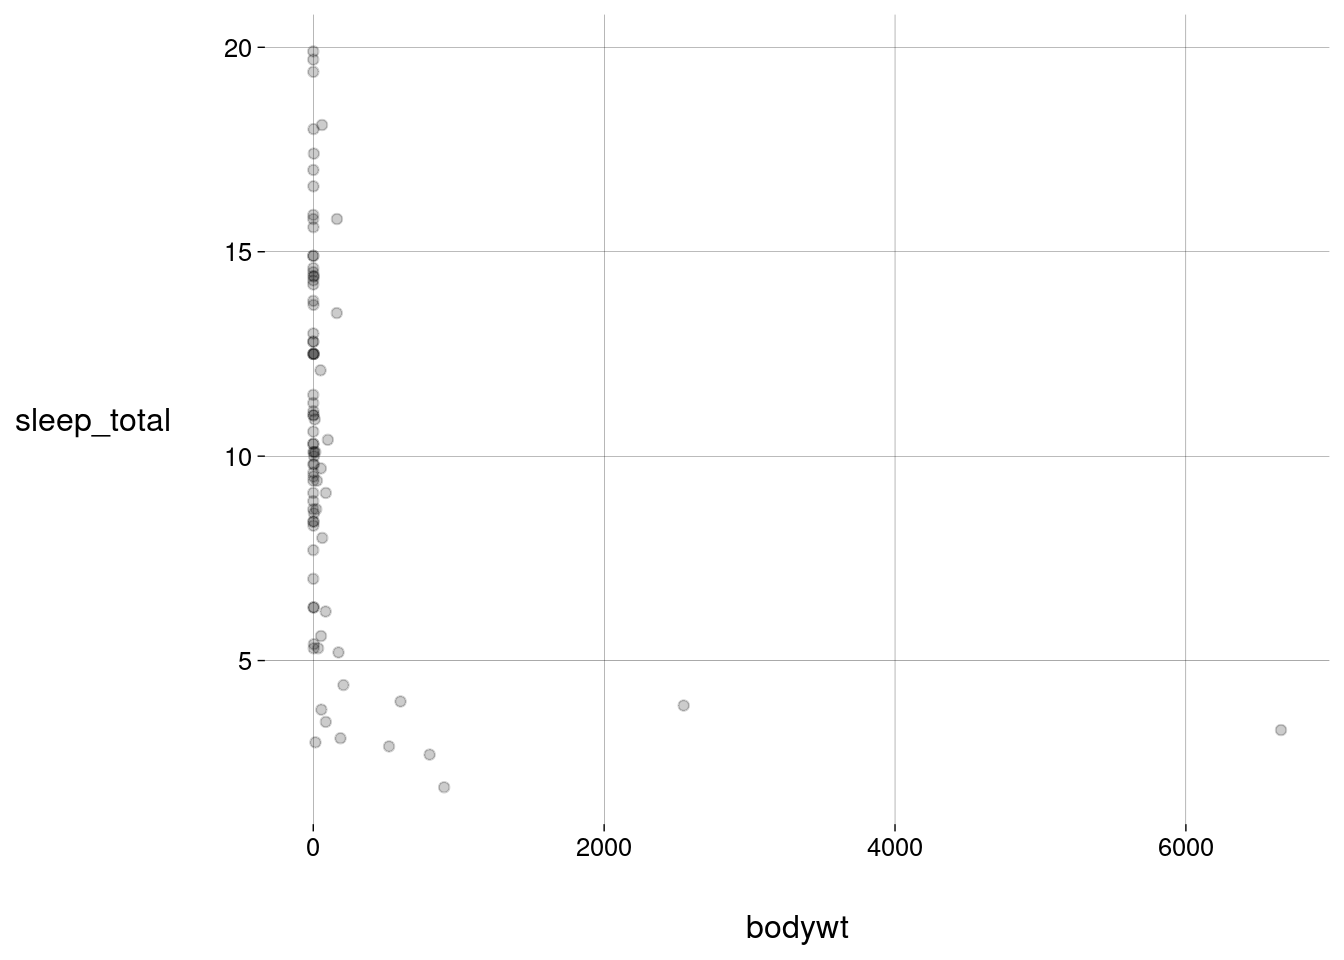
\includegraphics[width=1\linewidth]{_main_files/figure-latex/sono-peso-plot-alfa-1} \end{center}
\item
  Outra maneira é usar \texttt{geom\_jitter} em vez de \texttt{geom\_point}. ``\emph{Jitter}'' significa ``tremer''. As posições dos pontos são ligeiramente perturbadas, para evitar colisões. Perdemos precisão, mas a visualização fica melhor.

\begin{Shaded}
\begin{Highlighting}[]
\NormalTok{sono }\SpecialCharTok{\%\textgreater{}\%} 
  \FunctionTok{ggplot}\NormalTok{(}\FunctionTok{aes}\NormalTok{(}\AttributeTok{x =}\NormalTok{ bodywt, }\AttributeTok{y =}\NormalTok{ sleep\_total)) }\SpecialCharTok{+}
    \FunctionTok{geom\_jitter}\NormalTok{(}\AttributeTok{width =} \DecValTok{100}\NormalTok{)}
\end{Highlighting}
\end{Shaded}

  \begin{center}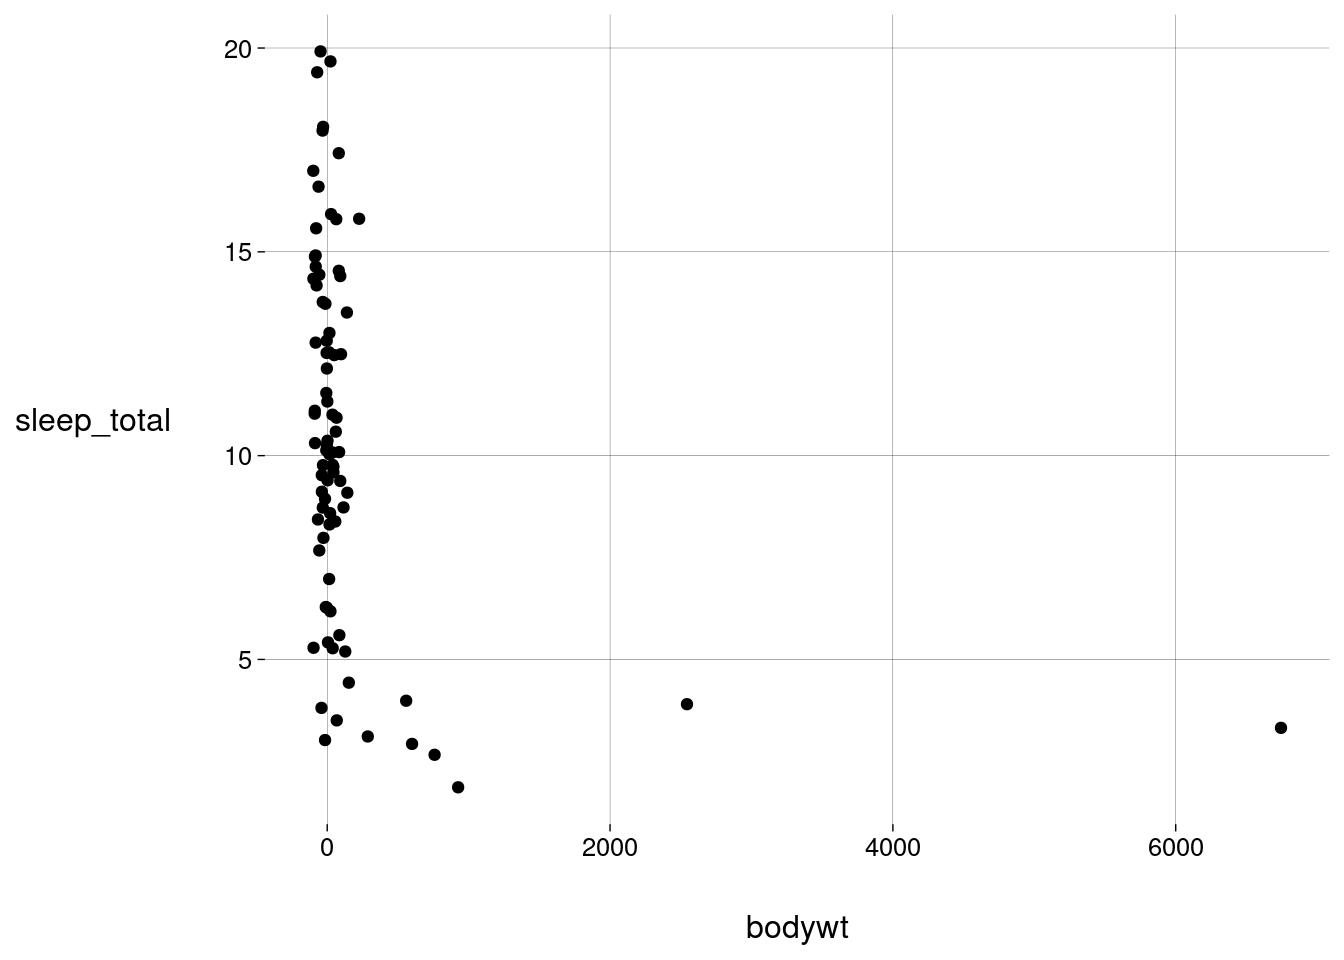
\includegraphics[width=1\linewidth]{_main_files/figure-latex/sono-peso-plot-jitter-1} \end{center}
\item
  Vamos mudar os limites do gráfico para nos concentrarmos nos animais menos pesados. Observe que {\hl{isto é um ajuste na escala}}.

\begin{Shaded}
\begin{Highlighting}[]
\NormalTok{sono }\SpecialCharTok{\%\textgreater{}\%} 
  \FunctionTok{ggplot}\NormalTok{(}\FunctionTok{aes}\NormalTok{(}\AttributeTok{x =}\NormalTok{ bodywt, }\AttributeTok{y =}\NormalTok{ sleep\_total)) }\SpecialCharTok{+}
    \FunctionTok{geom\_point}\NormalTok{() }\SpecialCharTok{+}
    \FunctionTok{scale\_x\_continuous}\NormalTok{(}\AttributeTok{limits =} \FunctionTok{c}\NormalTok{(}\DecValTok{0}\NormalTok{, }\DecValTok{200}\NormalTok{))}
\DocumentationTok{\#\# Warning: Removed 7 rows containing missing values (geom\_point).}
\end{Highlighting}
\end{Shaded}

  \begin{center}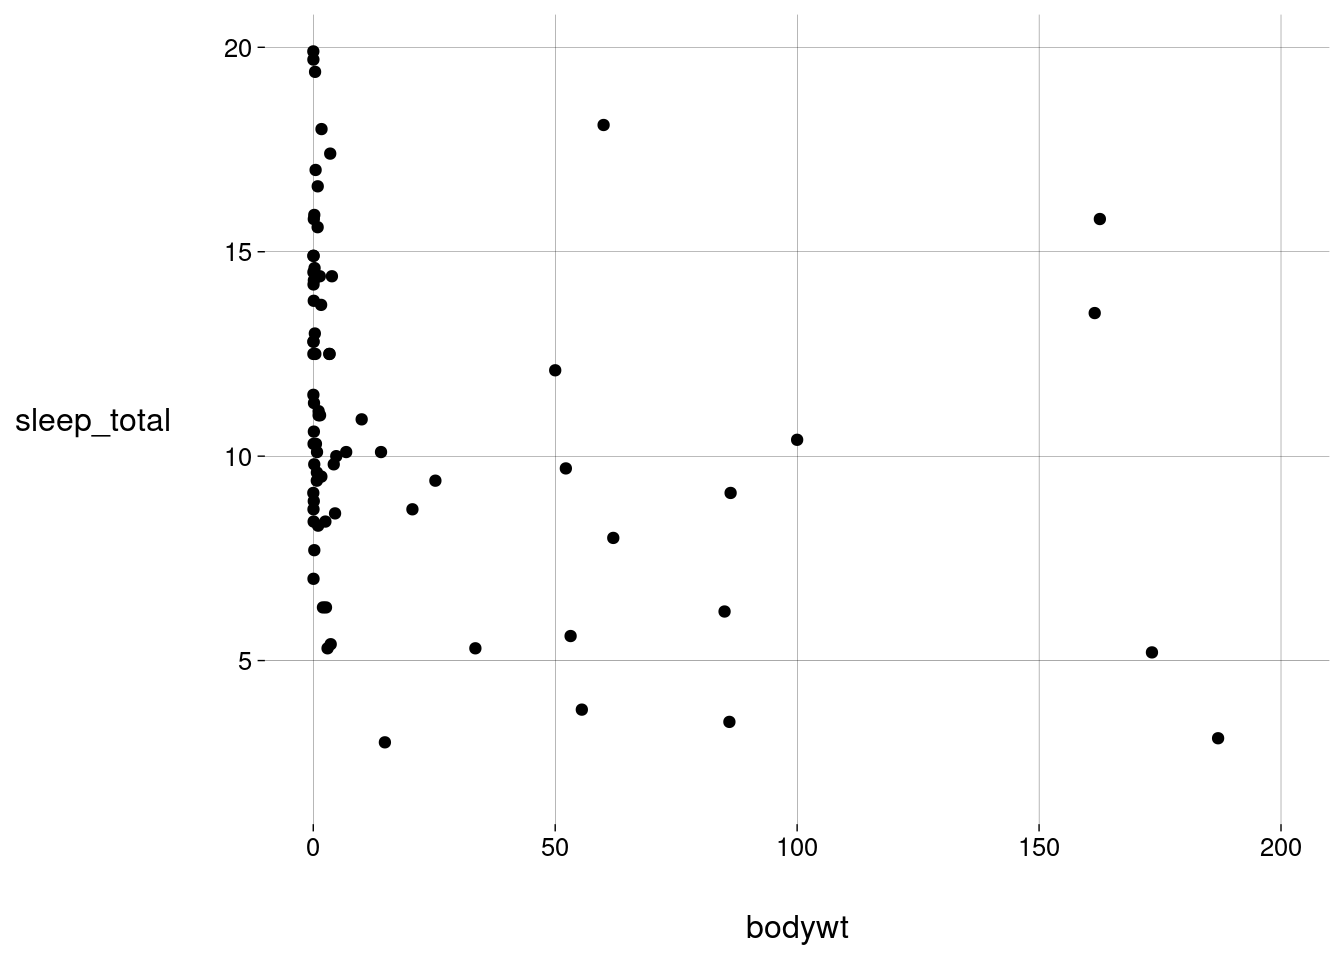
\includegraphics[width=1\linewidth]{_main_files/figure-latex/sono-peso-plot-3-1} \end{center}
\item
  Nestes limites, a relação entre horas de sono e peso não é mais tão pronunciada.
\end{itemize}

\hypertarget{horas-de-sono-e-peso-corporal-para-animais-pequenos}{%
\subsection{Horas de sono e peso corporal para animais pequenos}\label{horas-de-sono-e-peso-corporal-para-animais-pequenos}}

\begin{itemize}
\item
  Vamos restringir o gráfico a animais com no máximo $5$kg.

\begin{Shaded}
\begin{Highlighting}[]
\NormalTok{limite }\OtherTok{\textless{}{-}} \DecValTok{5}
\end{Highlighting}
\end{Shaded}
\item
  Em vez de mudar a escala do gráfico, vamos filtrar as linhas do \emph{data frame}:

\begin{Shaded}
\begin{Highlighting}[]
\NormalTok{sono }\SpecialCharTok{\%\textgreater{}\%} 
  \FunctionTok{filter}\NormalTok{(bodywt }\SpecialCharTok{\textless{}}\NormalTok{ limite) }\SpecialCharTok{\%\textgreater{}\%} 
  \FunctionTok{ggplot}\NormalTok{(}\FunctionTok{aes}\NormalTok{(}\AttributeTok{x =}\NormalTok{ bodywt, }\AttributeTok{y =}\NormalTok{ sleep\_total)) }\SpecialCharTok{+}
    \FunctionTok{geom\_point}\NormalTok{()}
\end{Highlighting}
\end{Shaded}

  \begin{center}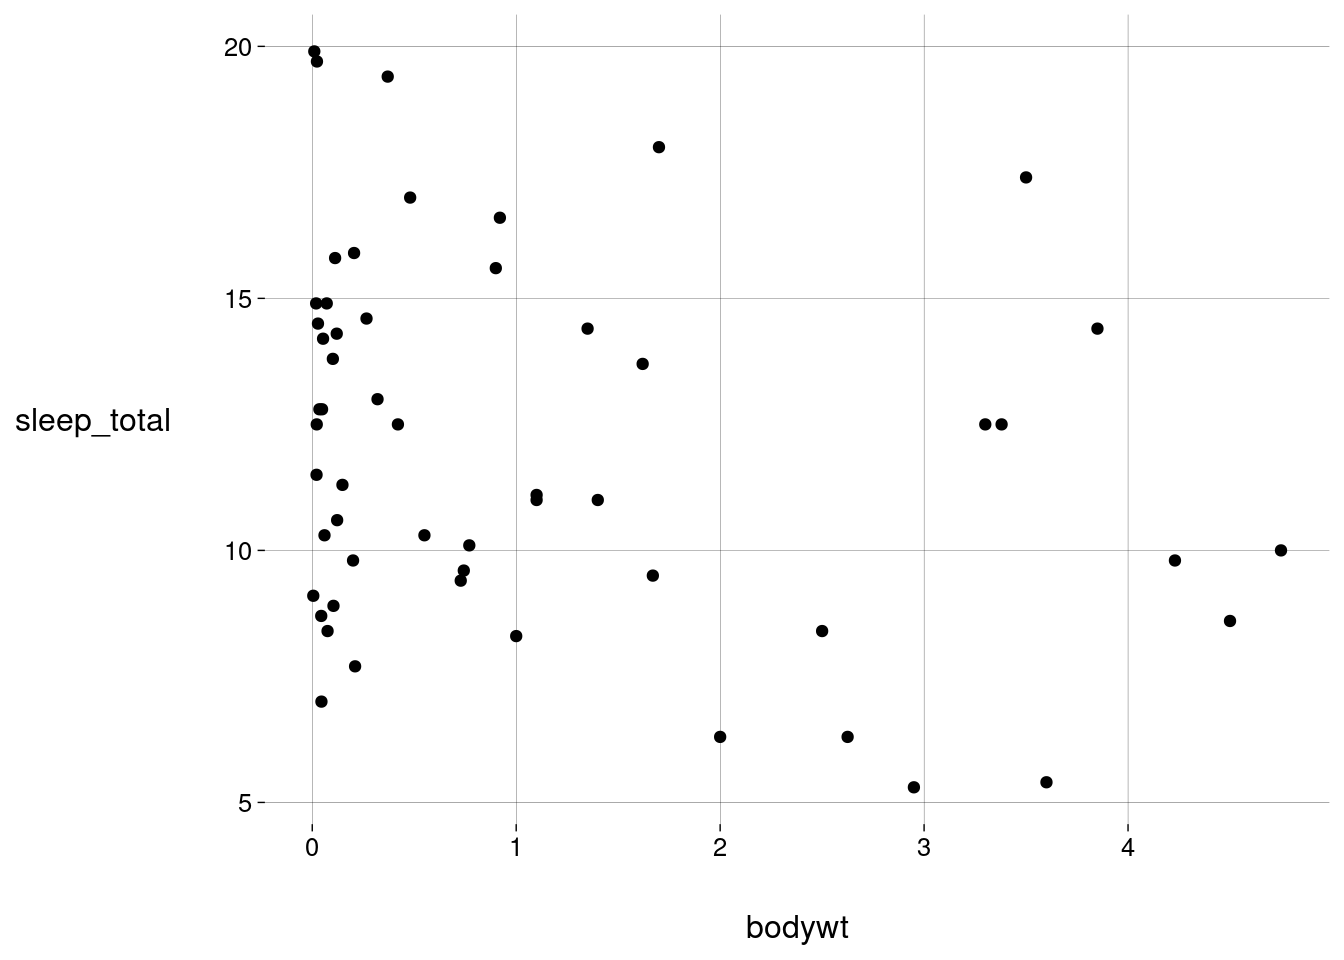
\includegraphics[width=1\linewidth]{_main_files/figure-latex/sono-peso-plot-pequenos-1} \end{center}
\end{itemize}

\hypertarget{incluindo-a-dieta}{%
\subsection{Incluindo a dieta}\label{incluindo-a-dieta}}

\begin{itemize}
\item
  Com a estética \texttt{color}. Observe como a legenda aparece automaticamente.

\begin{Shaded}
\begin{Highlighting}[]
\NormalTok{sono }\SpecialCharTok{\%\textgreater{}\%} 
  \FunctionTok{filter}\NormalTok{(bodywt }\SpecialCharTok{\textless{}}\NormalTok{ limite) }\SpecialCharTok{\%\textgreater{}\%} 
  \FunctionTok{ggplot}\NormalTok{(}\FunctionTok{aes}\NormalTok{(}\AttributeTok{x =}\NormalTok{ bodywt, }\AttributeTok{y =}\NormalTok{ sleep\_total, }\AttributeTok{color =}\NormalTok{ vore)) }\SpecialCharTok{+}
    \FunctionTok{geom\_point}\NormalTok{()}
\end{Highlighting}
\end{Shaded}

  \begin{center}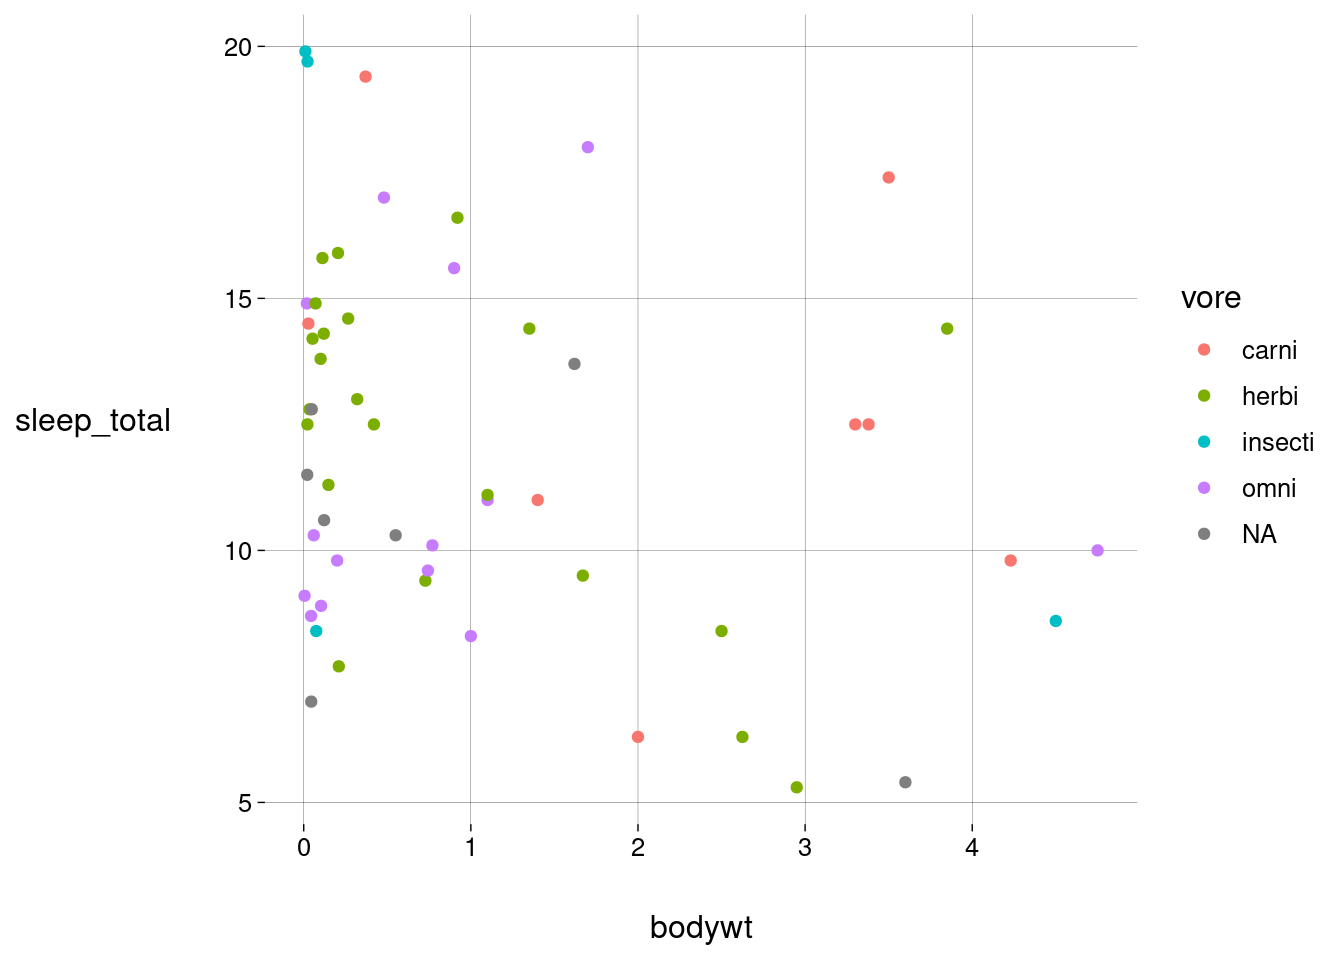
\includegraphics[width=1\linewidth]{_main_files/figure-latex/plot-sono-peso-dieta-1} \end{center}
\end{itemize}

\hypertarget{a-estuxe9tica-pode-ser-especificada-na-geom}{%
\subsection{\texorpdfstring{A estética pode ser especificada na \texttt{geom}}{A estética pode ser especificada na geom}}\label{a-estuxe9tica-pode-ser-especificada-na-geom}}

\begin{itemize}
\item
  Compare com o código anterior.

\begin{Shaded}
\begin{Highlighting}[]
\NormalTok{sono }\SpecialCharTok{\%\textgreater{}\%} 
  \FunctionTok{filter}\NormalTok{(bodywt }\SpecialCharTok{\textless{}}\NormalTok{ limite) }\SpecialCharTok{\%\textgreater{}\%} 
  \FunctionTok{ggplot}\NormalTok{() }\SpecialCharTok{+}
    \FunctionTok{geom\_point}\NormalTok{(}\FunctionTok{aes}\NormalTok{(}\AttributeTok{x =}\NormalTok{ bodywt, }\AttributeTok{y =}\NormalTok{ sleep\_total, }\AttributeTok{color =}\NormalTok{ vore))}
\end{Highlighting}
\end{Shaded}

  \begin{center}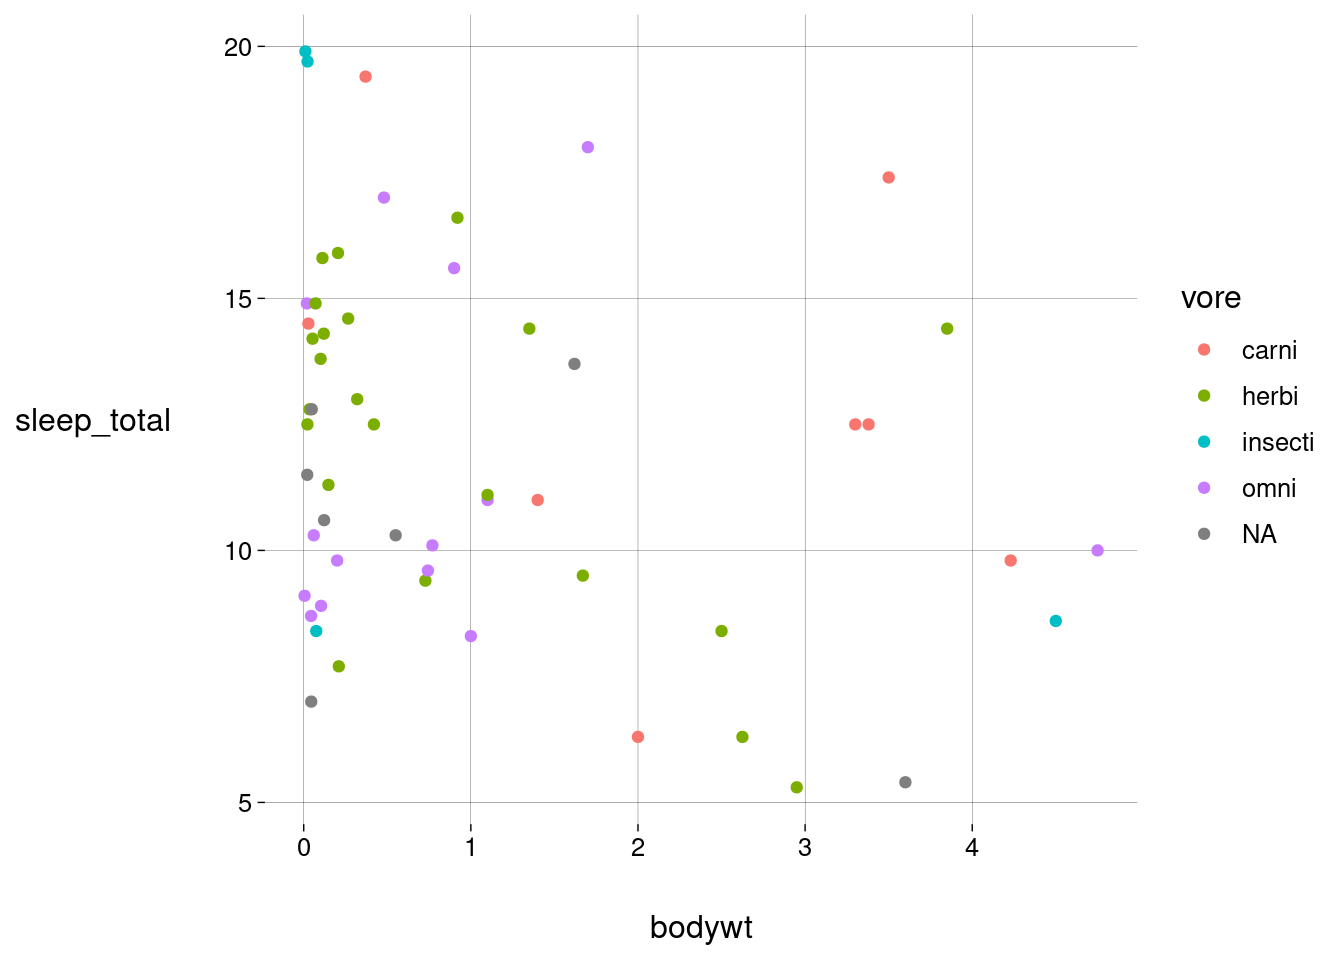
\includegraphics[width=1\linewidth]{_main_files/figure-latex/plot-sono-peso-dieta-geom-1} \end{center}
\item
  Fazendo deste modo, a estética só vale para uma geometria. Se você acrescentar outras geometrias (linhas, por exemplo), a estética não valerá para elas.
\end{itemize}

\hypertarget{aparuxeancia-fixa-ou-dependendo-de-variuxe1vel}{%
\subsection{Aparência fixa ou dependendo de variável?}\label{aparuxeancia-fixa-ou-dependendo-de-variuxe1vel}}

\begin{itemize}
\item
  Se for fixa, não é estética. Não representa informação.
\item
  Se depender de variável, é estética. Representa informação.
\item
  Compare o último \emph{chunk} acima com:

\begin{Shaded}
\begin{Highlighting}[]
\NormalTok{sono }\SpecialCharTok{\%\textgreater{}\%} 
  \FunctionTok{filter}\NormalTok{(bodywt }\SpecialCharTok{\textless{}}\NormalTok{ limite) }\SpecialCharTok{\%\textgreater{}\%} 
  \FunctionTok{ggplot}\NormalTok{() }\SpecialCharTok{+}
    \FunctionTok{geom\_point}\NormalTok{(}\FunctionTok{aes}\NormalTok{(}\AttributeTok{x =}\NormalTok{ bodywt, }\AttributeTok{y =}\NormalTok{ sleep\_total), }\AttributeTok{color =} \StringTok{\textquotesingle{}blue\textquotesingle{}}\NormalTok{)}
\end{Highlighting}
\end{Shaded}

  \begin{center}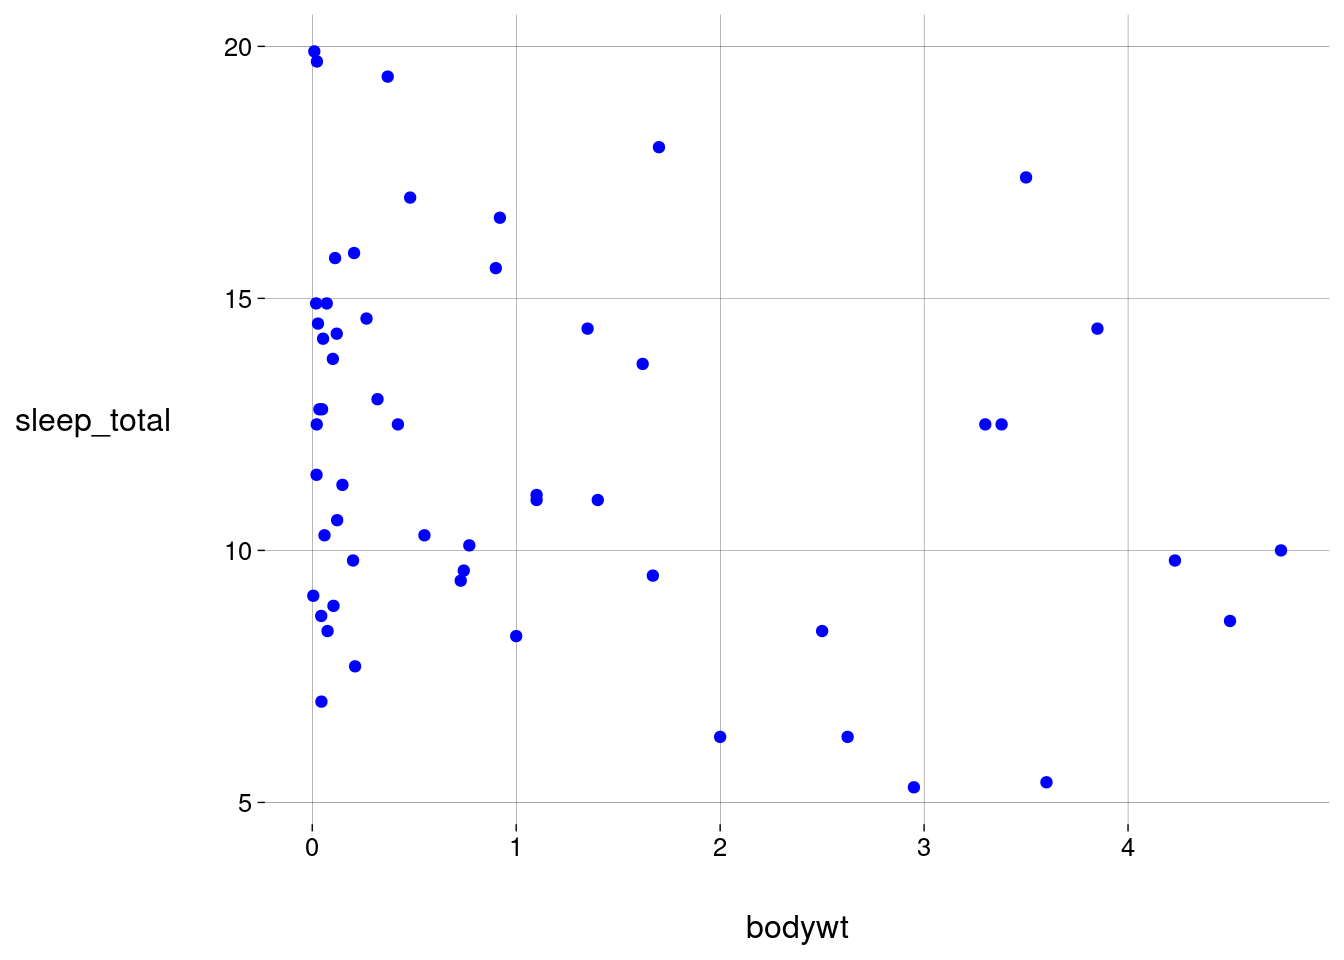
\includegraphics[width=1\linewidth]{_main_files/figure-latex/plot-sono-peso-cor-1} \end{center}
\item
  Se for uma estética, precisa estar {\hl{associada a uma variável}}, não a um valor fixo. Um erro comum seria fazer:

\begin{Shaded}
\begin{Highlighting}[]
\NormalTok{sono }\SpecialCharTok{\%\textgreater{}\%} 
  \FunctionTok{filter}\NormalTok{(bodywt }\SpecialCharTok{\textless{}}\NormalTok{ limite) }\SpecialCharTok{\%\textgreater{}\%} 
  \FunctionTok{ggplot}\NormalTok{() }\SpecialCharTok{+}
    \FunctionTok{geom\_point}\NormalTok{(}\FunctionTok{aes}\NormalTok{(}\AttributeTok{x =}\NormalTok{ bodywt, }\AttributeTok{y =}\NormalTok{ sleep\_total, }\AttributeTok{color =} \StringTok{\textquotesingle{}blue\textquotesingle{}}\NormalTok{))}
\end{Highlighting}
\end{Shaded}

  \begin{center}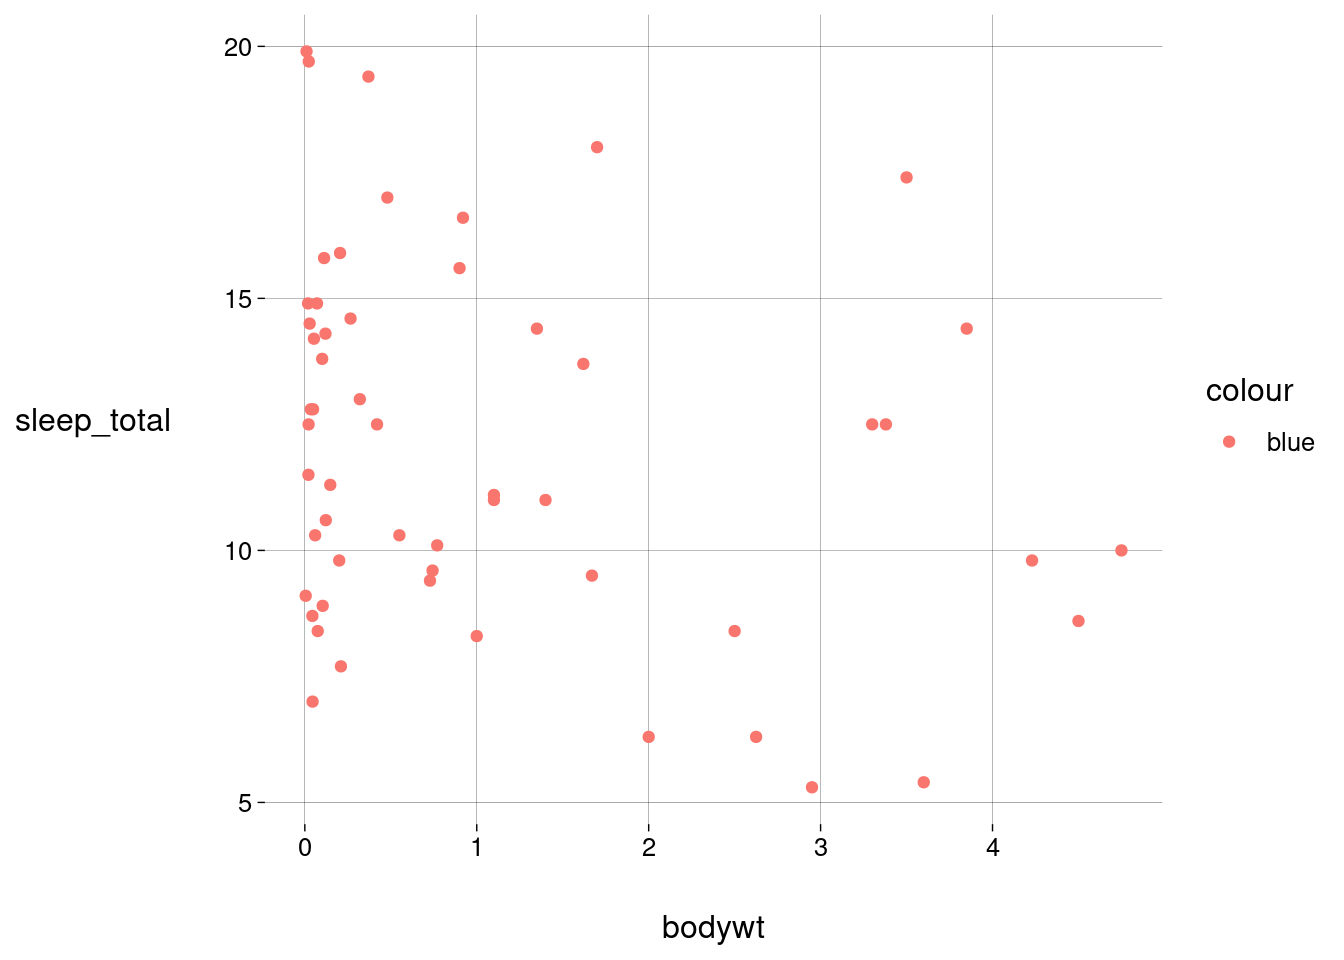
\includegraphics[width=1\linewidth]{_main_files/figure-latex/plot-sono-peso-cor-erro-1} \end{center}
\end{itemize}

\hypertarget{uma-correlauxe7uxe3o-mais-clara}{%
\subsection{Uma correlação mais clara}\label{uma-correlauxe7uxe3o-mais-clara}}

\begin{itemize}
\item
  Peso cerebral versus peso corporal:

\begin{Shaded}
\begin{Highlighting}[]
\NormalTok{sono }\SpecialCharTok{\%\textgreater{}\%} 
  \FunctionTok{ggplot}\NormalTok{(}\FunctionTok{aes}\NormalTok{(}\AttributeTok{x =}\NormalTok{ bodywt, }\AttributeTok{y =}\NormalTok{ brainwt)) }\SpecialCharTok{+}
    \FunctionTok{geom\_point}\NormalTok{()}
\DocumentationTok{\#\# Warning: Removed 27 rows containing missing values (geom\_point).}
\end{Highlighting}
\end{Shaded}

  \begin{center}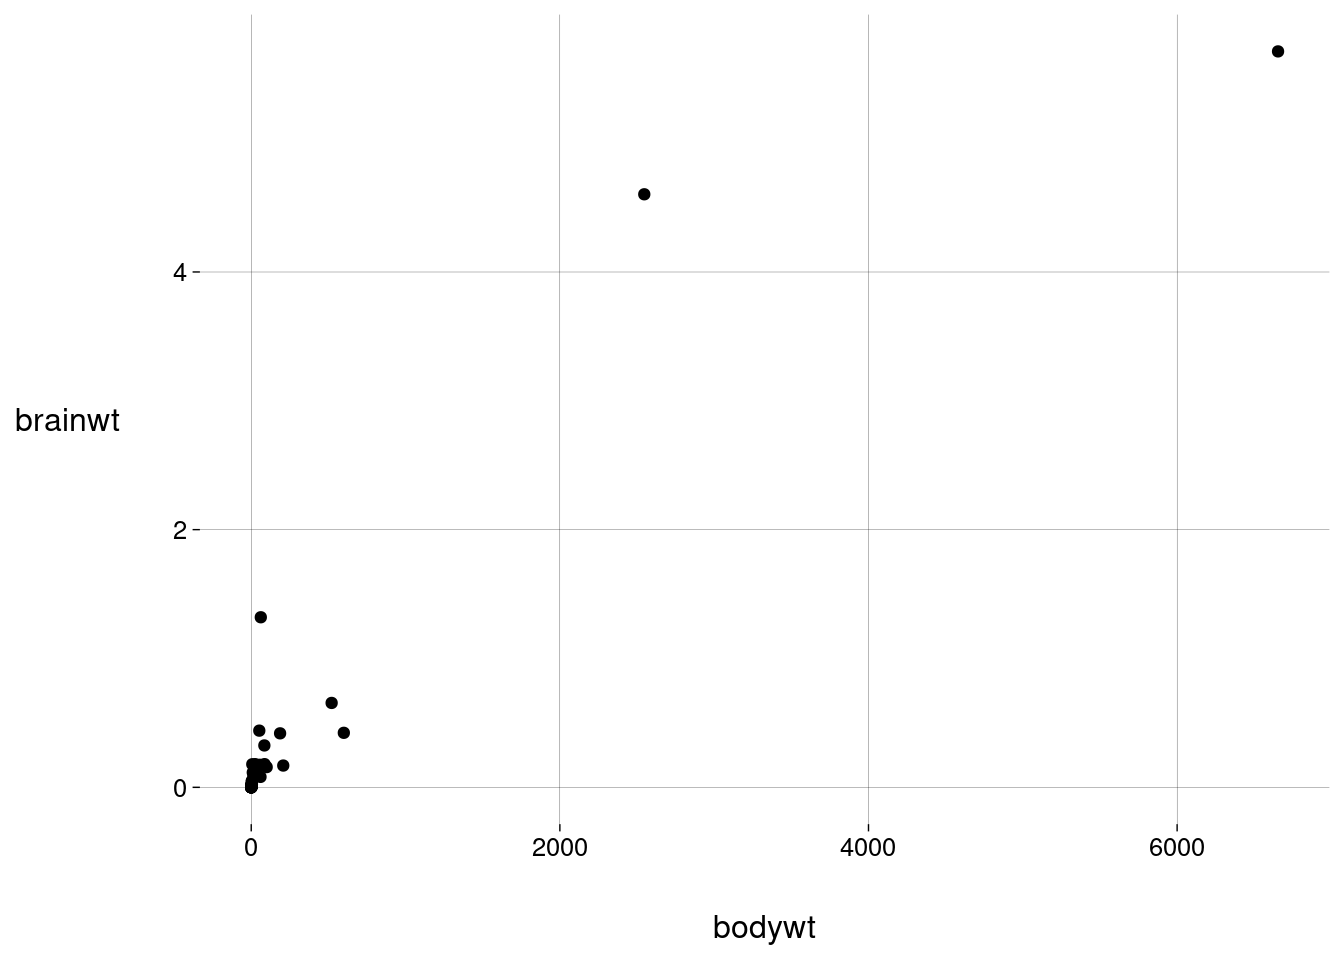
\includegraphics[width=1\linewidth]{_main_files/figure-latex/cerebro-corpo-1} \end{center}
\item
  A mensagem de aviso (\emph{warning}) diz que há $27$ valores faltantes (\texttt{NA}) em \texttt{bodywt} ou \texttt{brainwt}. De fato:

\begin{Shaded}
\begin{Highlighting}[]
\NormalTok{sono }\SpecialCharTok{\%\textgreater{}\%} 
  \FunctionTok{filter}\NormalTok{(}\FunctionTok{is.na}\NormalTok{(bodywt)) }\SpecialCharTok{\%\textgreater{}\%} 
  \FunctionTok{count}\NormalTok{()}
\DocumentationTok{\#\# \# A tibble: 1 x 1}
\DocumentationTok{\#\#       n}
\DocumentationTok{\#\#   \textless{}int\textgreater{}}
\DocumentationTok{\#\# 1     0}
\end{Highlighting}
\end{Shaded}

\begin{Shaded}
\begin{Highlighting}[]
\NormalTok{sono }\SpecialCharTok{\%\textgreater{}\%} 
  \FunctionTok{filter}\NormalTok{(}\FunctionTok{is.na}\NormalTok{(brainwt)) }\SpecialCharTok{\%\textgreater{}\%} 
  \FunctionTok{count}\NormalTok{()}
\DocumentationTok{\#\# \# A tibble: 1 x 1}
\DocumentationTok{\#\#       n}
\DocumentationTok{\#\#   \textless{}int\textgreater{}}
\DocumentationTok{\#\# 1    27}
\end{Highlighting}
\end{Shaded}
\item
  Vamos restringir aos animais mais leves e mudar a opacidade:

\begin{Shaded}
\begin{Highlighting}[]
\NormalTok{sono }\SpecialCharTok{\%\textgreater{}\%} 
  \FunctionTok{filter}\NormalTok{(bodywt }\SpecialCharTok{\textless{}}\NormalTok{ limite) }\SpecialCharTok{\%\textgreater{}\%} 
  \FunctionTok{ggplot}\NormalTok{(}\FunctionTok{aes}\NormalTok{(}\AttributeTok{x =}\NormalTok{ bodywt, }\AttributeTok{y =}\NormalTok{ brainwt)) }\SpecialCharTok{+}
    \FunctionTok{geom\_point}\NormalTok{(}\AttributeTok{alpha =}\NormalTok{ .}\DecValTok{5}\NormalTok{)}
\DocumentationTok{\#\# Warning: Removed 18 rows containing missing values (geom\_point).}
\end{Highlighting}
\end{Shaded}

  \begin{center}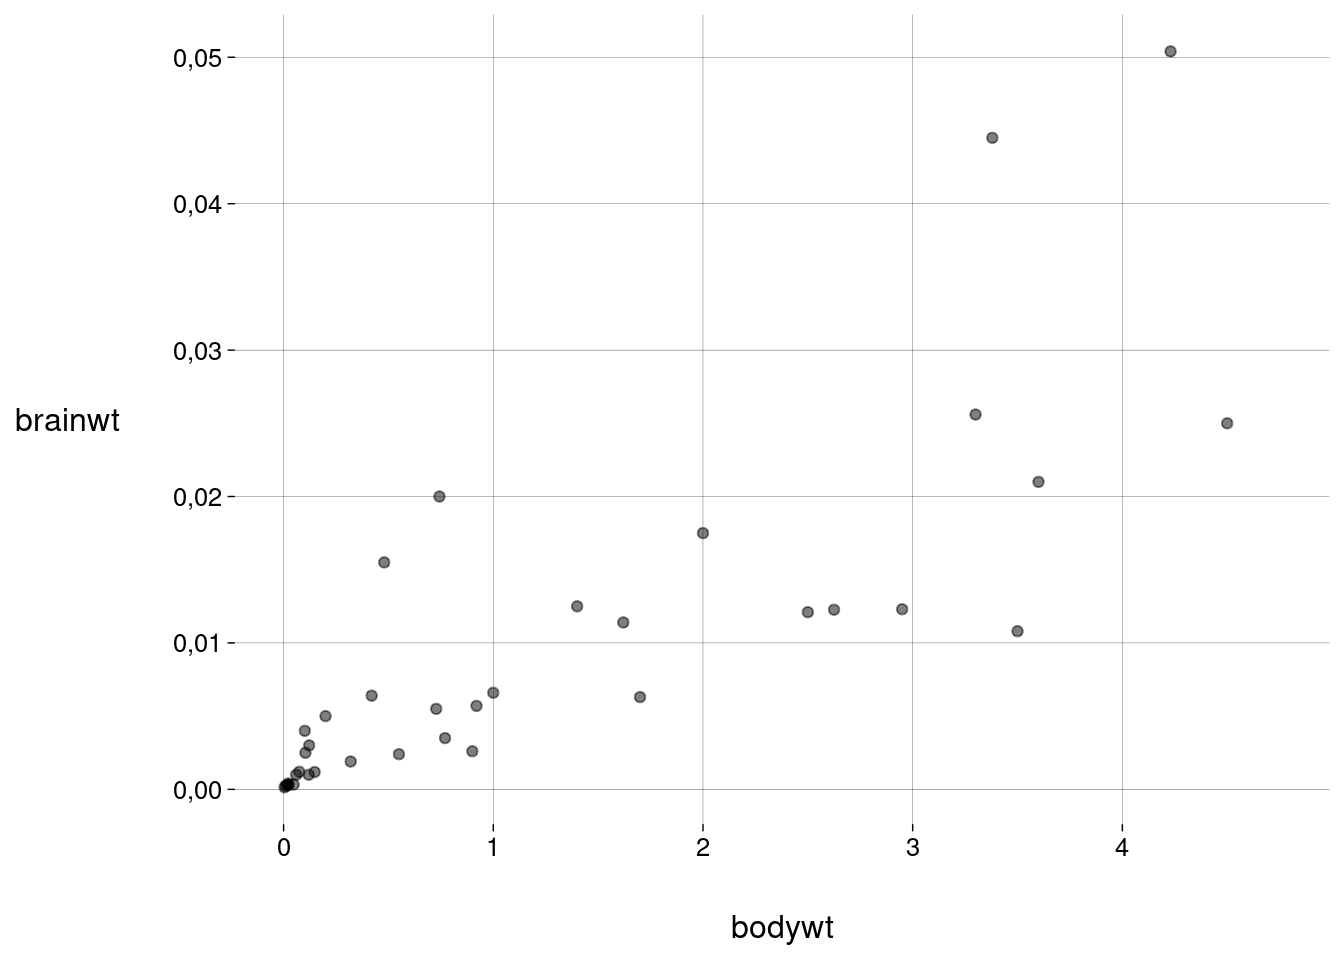
\includegraphics[width=1\linewidth]{_main_files/figure-latex/cerebro-corpo-2-1} \end{center}
\item
  Vamos incluir horas de sono e dieta. Observe as estéticas usadas.

\begin{Shaded}
\begin{Highlighting}[]
\NormalTok{sono }\SpecialCharTok{\%\textgreater{}\%} 
  \FunctionTok{filter}\NormalTok{(bodywt }\SpecialCharTok{\textless{}}\NormalTok{ limite) }\SpecialCharTok{\%\textgreater{}\%} 
  \FunctionTok{ggplot}\NormalTok{(}
    \FunctionTok{aes}\NormalTok{(}
      \AttributeTok{x =}\NormalTok{ bodywt, }
      \AttributeTok{y =}\NormalTok{ brainwt,}
      \AttributeTok{size =}\NormalTok{ sleep\_total,}
      \AttributeTok{color =}\NormalTok{ vore}
\NormalTok{    )}
\NormalTok{  ) }\SpecialCharTok{+}
    \FunctionTok{geom\_point}\NormalTok{(}\AttributeTok{alpha =}\NormalTok{ .}\DecValTok{5}\NormalTok{)}
\DocumentationTok{\#\# Warning: Removed 18 rows containing missing values (geom\_point).}
\end{Highlighting}
\end{Shaded}

  \begin{center}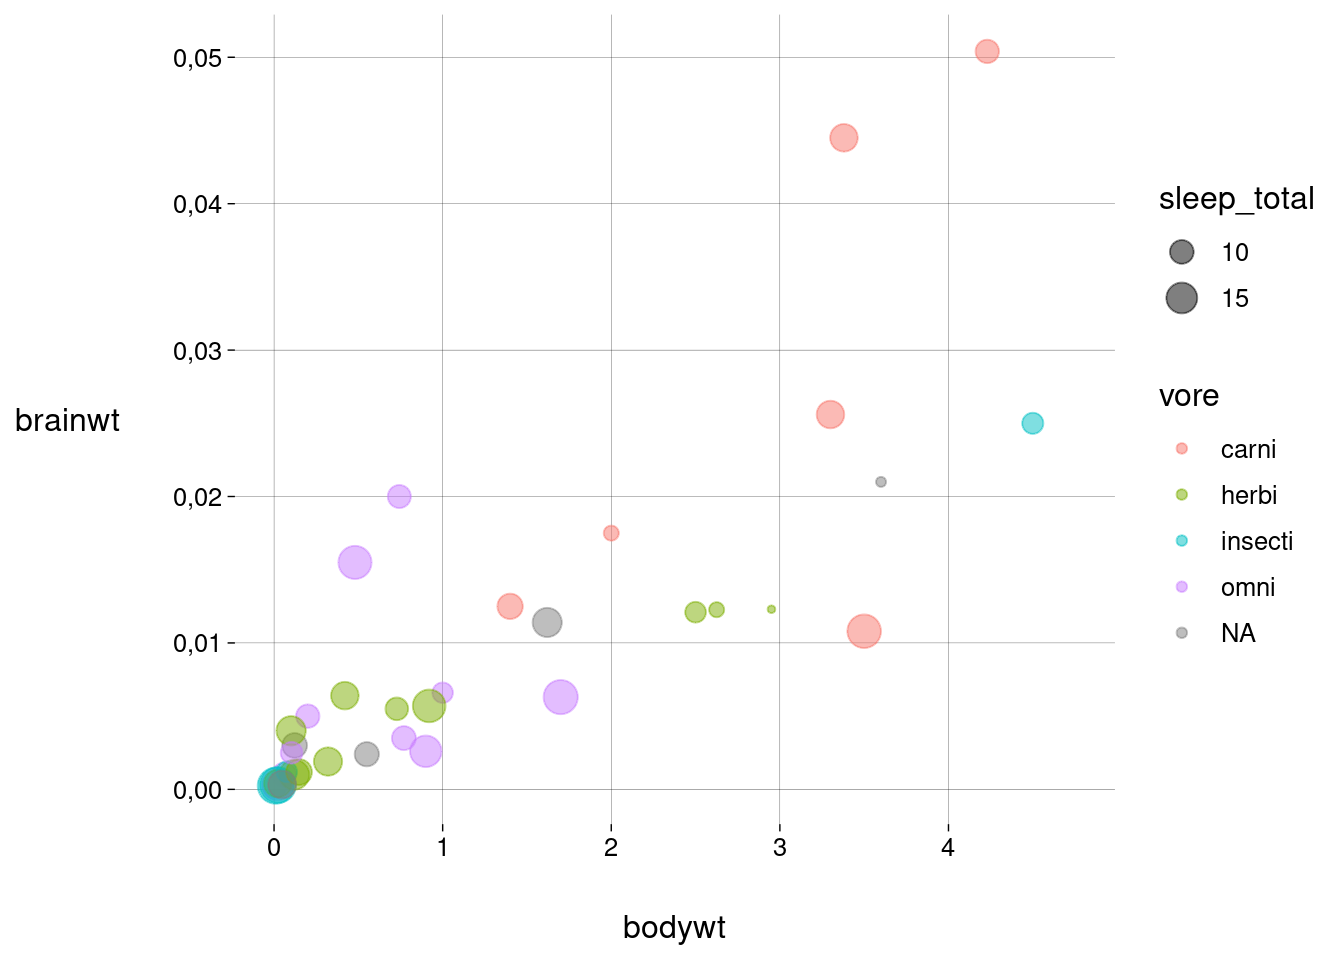
\includegraphics[width=1\linewidth]{_main_files/figure-latex/cerebro-corpo-3-1} \end{center}
\item
  Vamos mudar a escala dos tamanhos e incluir rótulos:

\begin{Shaded}
\begin{Highlighting}[]
\NormalTok{grafico }\OtherTok{\textless{}{-}}\NormalTok{ sono }\SpecialCharTok{\%\textgreater{}\%} 
  \FunctionTok{filter}\NormalTok{(bodywt }\SpecialCharTok{\textless{}}\NormalTok{ limite) }\SpecialCharTok{\%\textgreater{}\%} 
  \FunctionTok{ggplot}\NormalTok{(}
    \FunctionTok{aes}\NormalTok{(}
      \AttributeTok{x =}\NormalTok{ bodywt, }
      \AttributeTok{y =}\NormalTok{ brainwt,}
      \AttributeTok{size =}\NormalTok{ sleep\_total,}
      \AttributeTok{color =}\NormalTok{ vore}
\NormalTok{    )}
\NormalTok{  ) }\SpecialCharTok{+}
    \FunctionTok{geom\_point}\NormalTok{(}\AttributeTok{alpha =}\NormalTok{ .}\DecValTok{5}\NormalTok{) }\SpecialCharTok{+}
    \FunctionTok{scale\_size}\NormalTok{(}
      \AttributeTok{breaks =} \FunctionTok{seq}\NormalTok{(}\DecValTok{0}\NormalTok{, }\DecValTok{24}\NormalTok{, }\DecValTok{4}\NormalTok{)}
\NormalTok{    ) }\SpecialCharTok{+}
    \FunctionTok{labs}\NormalTok{(}
      \AttributeTok{title =} \StringTok{\textquotesingle{}Peso do cérebro versus peso corporal\textquotesingle{}}\NormalTok{,}
      \AttributeTok{subtitle =} \FunctionTok{paste0}\NormalTok{(}
        \StringTok{\textquotesingle{}para mamíferos com menos de \textquotesingle{}}\NormalTok{, }
\NormalTok{        limite, }
        \StringTok{\textquotesingle{} kg\textquotesingle{}}
\NormalTok{      ),}
      \AttributeTok{caption =} \StringTok{\textquotesingle{}Fonte: dataset \textasciigrave{}msleep\textasciigrave{}\textquotesingle{}}\NormalTok{,}
      \AttributeTok{x =} \StringTok{\textquotesingle{}Peso corporal (kg)\textquotesingle{}}\NormalTok{,}
      \AttributeTok{y =} \StringTok{\textquotesingle{}Peso do}\SpecialCharTok{\textbackslash{}n}\StringTok{ cérebro (kg)\textquotesingle{}}\NormalTok{,}
      \AttributeTok{color =} \StringTok{\textquotesingle{}Dieta\textquotesingle{}}\NormalTok{,}
      \AttributeTok{size =} \StringTok{\textquotesingle{}Horas}\SpecialCharTok{\textbackslash{}n}\StringTok{de sono\textquotesingle{}}
\NormalTok{    )}

\NormalTok{grafico}
\DocumentationTok{\#\# Warning: Removed 18 rows containing missing values (geom\_point).}
\end{Highlighting}
\end{Shaded}

  \begin{center}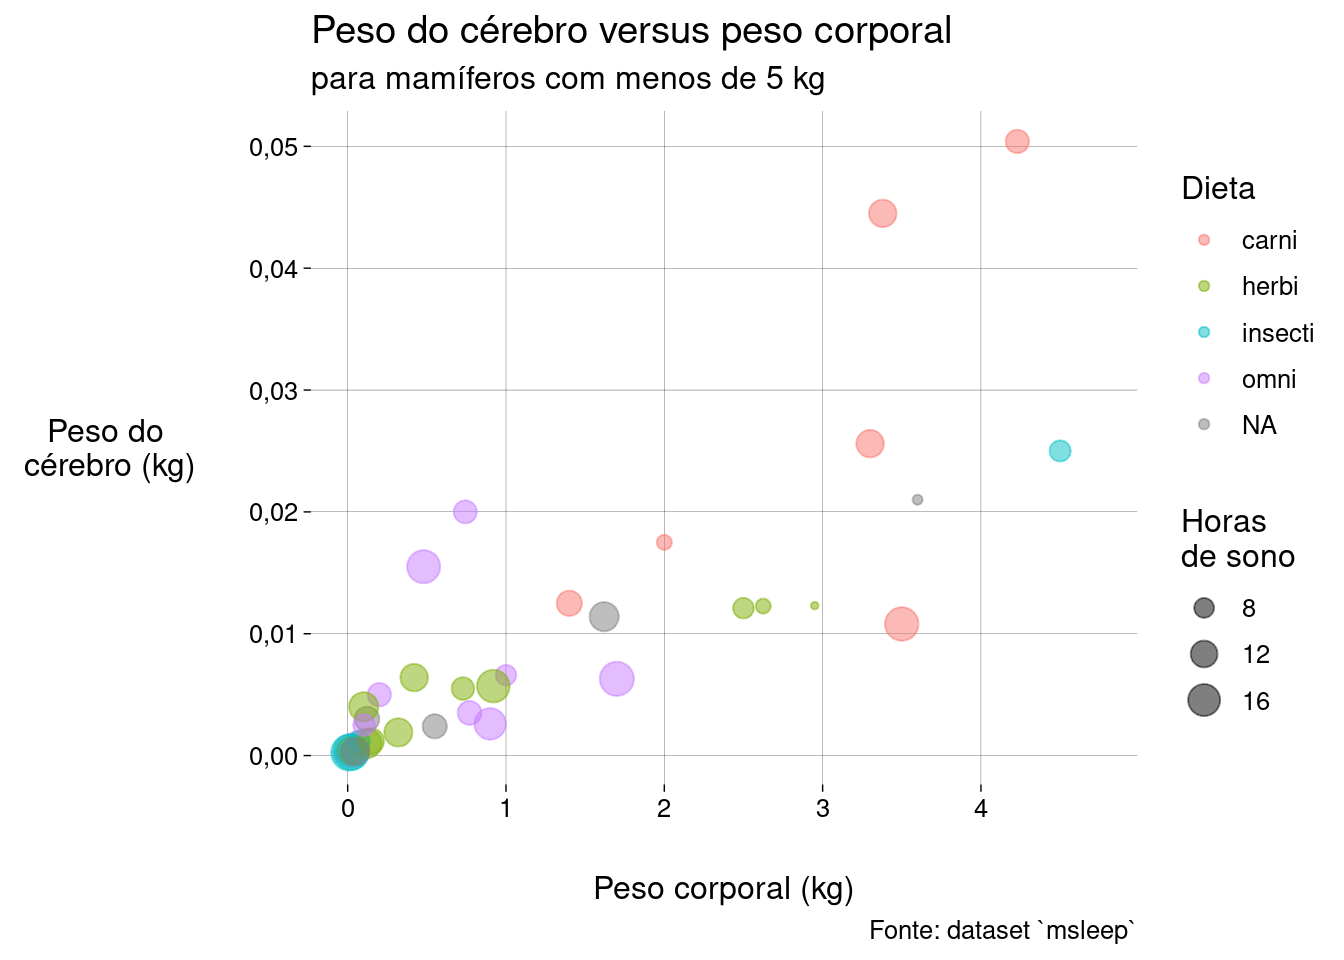
\includegraphics[width=1\linewidth]{_main_files/figure-latex/cerebro-corpo-4-1} \end{center}
\item
  Vamos mudar as cores usadas para a dieta, usando uma escala diferente.

\begin{Shaded}
\begin{Highlighting}[]
\NormalTok{grafico2 }\OtherTok{\textless{}{-}}\NormalTok{ grafico }\SpecialCharTok{+}
  \FunctionTok{scale\_color\_discrete}\NormalTok{(}
    \AttributeTok{palette =} \StringTok{\textquotesingle{}RdBu\textquotesingle{}}\NormalTok{,}
    \AttributeTok{na.value =} \StringTok{\textquotesingle{}black\textquotesingle{}}\NormalTok{,}
    \AttributeTok{type =}\NormalTok{ scale\_color\_brewer}
\NormalTok{  )}

\NormalTok{grafico2}
\DocumentationTok{\#\# Warning: Removed 18 rows containing missing values (geom\_point).}
\end{Highlighting}
\end{Shaded}

  \begin{center}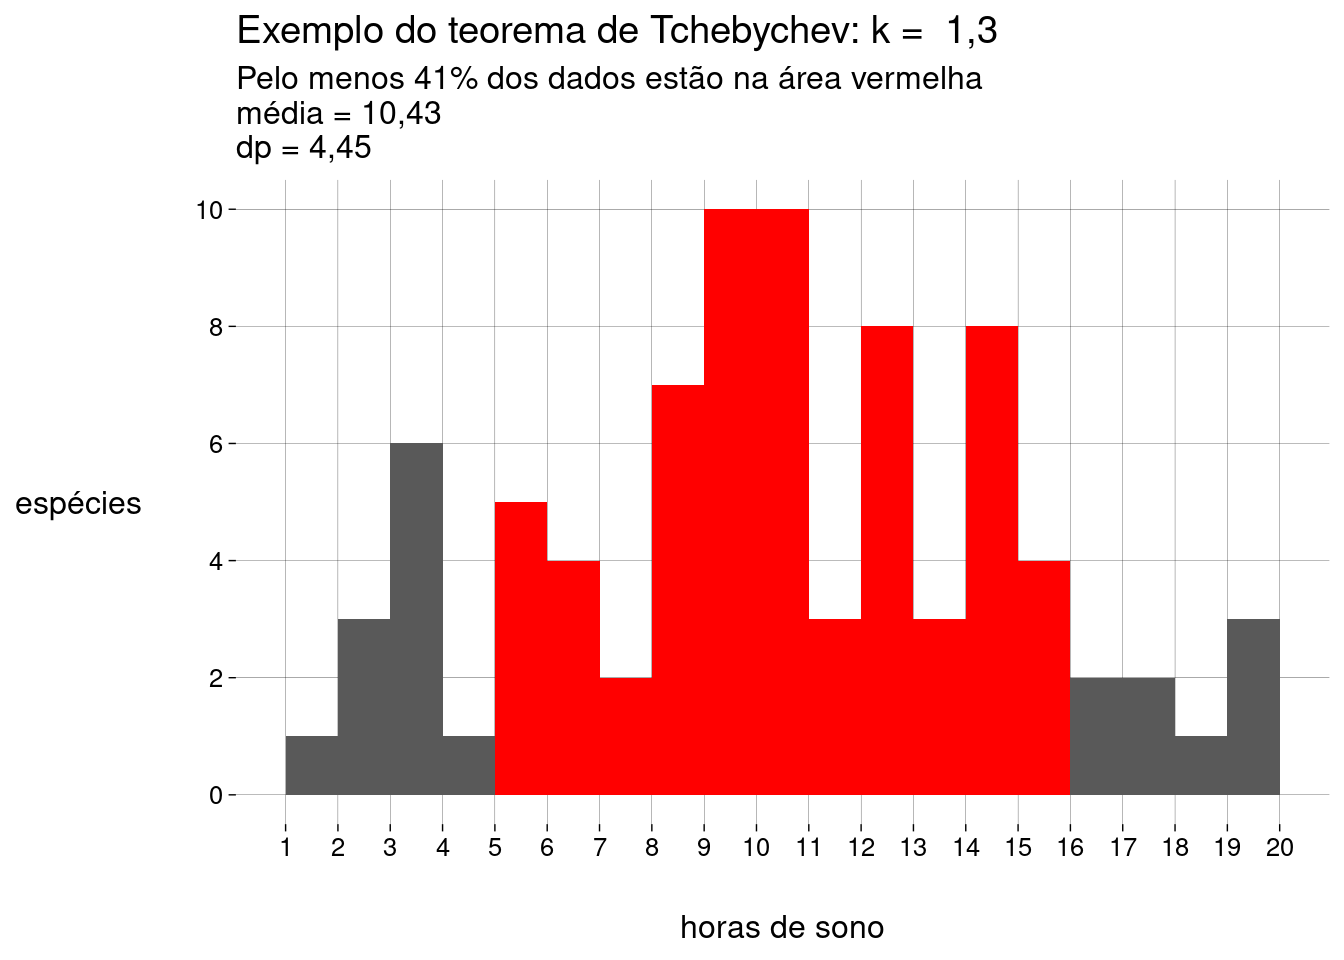
\includegraphics[width=1\linewidth]{_main_files/figure-latex/unnamed-chunk-21-1} \end{center}
\item
  Observe como usamos o gráfico já salvo na variável \texttt{grafico} e simplesmente acrescentamos a nova escala. Este tipo de ``montagem'' de gráficos \texttt{ggplot2} é bem conveniente, para evitar repetição de código.
\item
  Um último ajuste na aparência: os pontos na legenda ``Dieta'' estão pequenos demais. Quase não identificamos as cores deles.

  Vamos usar a função \texttt{guides} para modificar (\emph{override}) a estética \texttt{color} --- {\hl{apenas na legenda, não nos pontos mostrados no gráfico, cujos tamanhos representam o número de horas de sono}} --- tornando o tamanho maior. \href{https://ggplot2-book.org/scale-colour.html\#guide_legend}{Leia mais sobre \texttt{override.aes}neste \emph{link} (em inglês)}.

\begin{Shaded}
\begin{Highlighting}[]
\NormalTok{grafico3 }\OtherTok{\textless{}{-}}\NormalTok{ grafico2 }\SpecialCharTok{+}
  \FunctionTok{guides}\NormalTok{(}\AttributeTok{color =} \FunctionTok{guide\_legend}\NormalTok{(}\AttributeTok{override.aes =} \FunctionTok{list}\NormalTok{(}\AttributeTok{size =} \DecValTok{10}\NormalTok{)))}

\NormalTok{grafico3}
\DocumentationTok{\#\# Warning: Removed 18 rows containing missing values (geom\_point).}
\end{Highlighting}
\end{Shaded}

  \begin{center}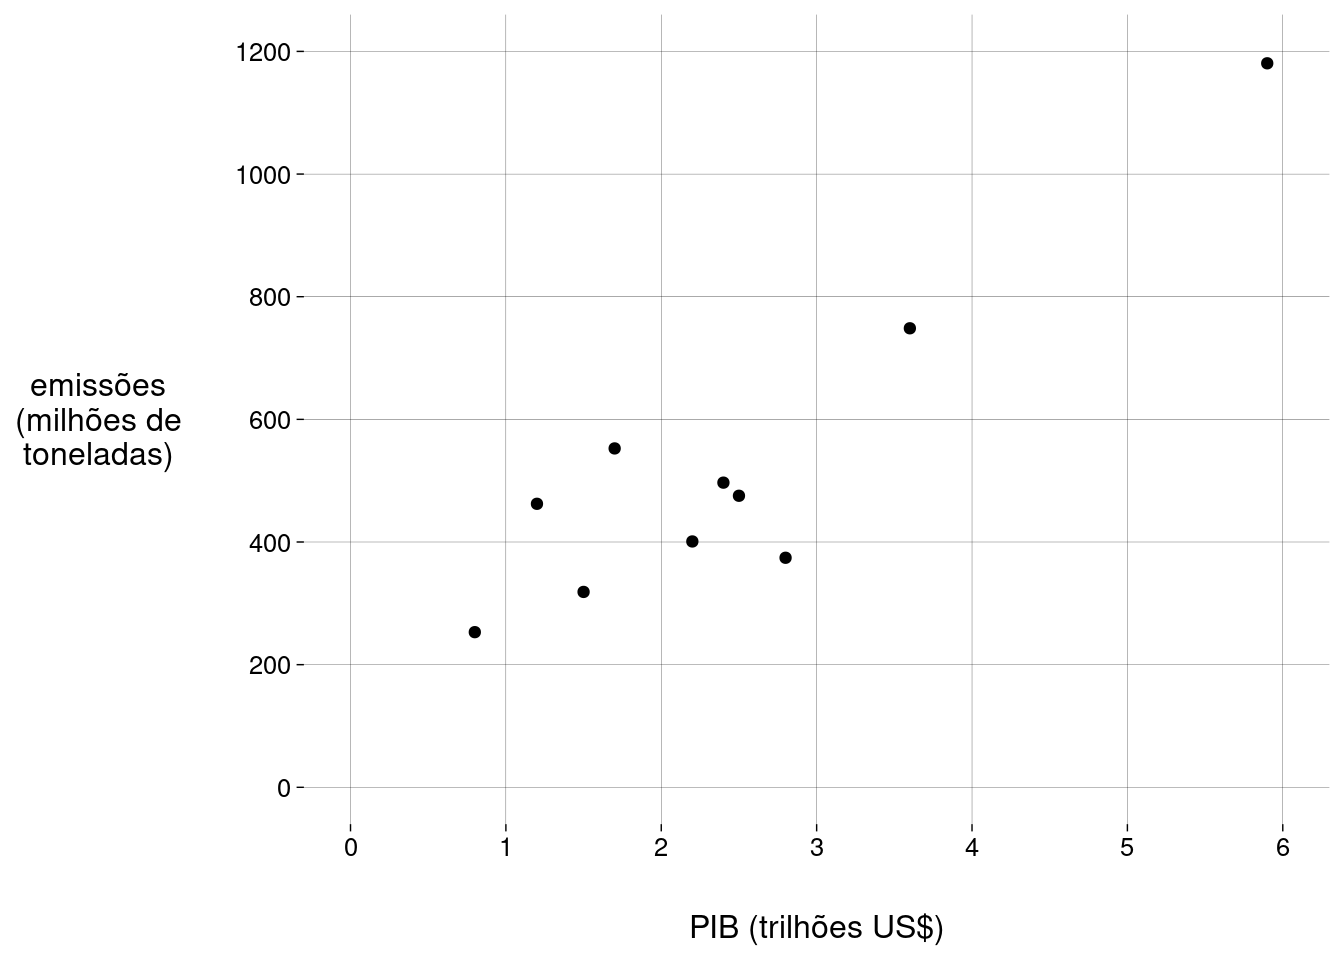
\includegraphics[width=1\linewidth]{_main_files/figure-latex/unnamed-chunk-22-1} \end{center}
\item
  Agora podemos finalmente comentar sobre a informação que o gráfico mostra sobre os dados:

  \begin{itemize}
  \item
    De fato, existe uma correlação entre peso cerebral e peso corporal: quanto maior o peso corporal, maior o peso cerebral. Nada surprenndente.
  \item
    \protect\hypertarget{grafico4}{}{} Podemos fazer o \texttt{ggplot2} traçar uma reta de regressão com a geometria \texttt{geom\_smooth}. Vamos falar mais sobre correlação \protect\hyperlink{correlacao}{em um capítulo futuro}.

\begin{Shaded}
\begin{Highlighting}[]
\NormalTok{grafico4 }\OtherTok{\textless{}{-}}\NormalTok{ grafico3 }\SpecialCharTok{+}
  \FunctionTok{geom\_smooth}\NormalTok{(}
    \FunctionTok{aes}\NormalTok{(}\AttributeTok{group =} \DecValTok{1}\NormalTok{), }
    \AttributeTok{show.legend =} \ConstantTok{FALSE}\NormalTok{,}
    \AttributeTok{method =} \StringTok{\textquotesingle{}lm\textquotesingle{}}\NormalTok{, }
    \AttributeTok{se =} \ConstantTok{FALSE}
\NormalTok{  )}

\NormalTok{grafico4}
\DocumentationTok{\#\# \textasciigrave{}geom\_smooth()\textasciigrave{} using formula \textquotesingle{}y \textasciitilde{} x\textquotesingle{}}
\DocumentationTok{\#\# Warning: Removed 18 rows containing non{-}finite values (stat\_smooth).}
\DocumentationTok{\#\# Warning: Removed 18 rows containing missing values (geom\_point).}
\end{Highlighting}
\end{Shaded}

    \begin{center}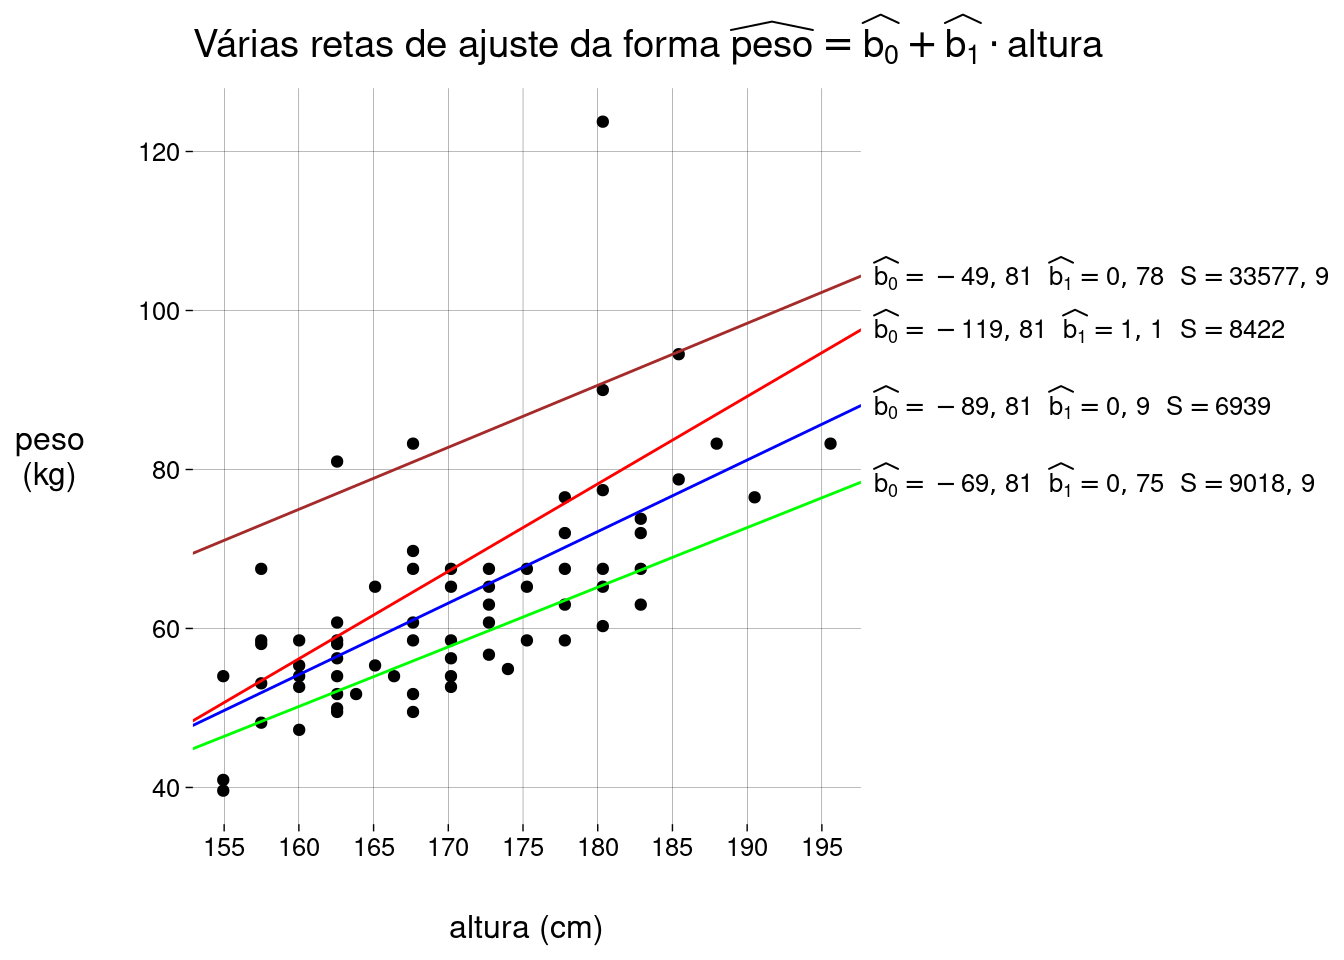
\includegraphics[width=1\linewidth]{_main_files/figure-latex/unnamed-chunk-23-1} \end{center}
  \item
    Todos os carnívoros têm peso corporal maior que $1$kg e peso cerebral maior ou igual a $10$g.
  \item
    Só um carnívoro dorme $8$ horas ou menos. Qual?
  \item
    Todos os insetívoros --- com exceção de um (qual?) --- são muito leves e dormem muito.
  \item
    Todos os onívoros têm menos de $2$kg de peso corporal e $20$g ou menos de peso cerebral.
  \end{itemize}
\end{itemize}

\hypertarget{vuxeddeo-2-2}{%
\section{Vídeo 2}\label{vuxeddeo-2-2}}

\begin{center} \url{https://youtu.be/c-LoZ9e8xWc} \end{center}

\hypertarget{histogramas-e-cia.}{%
\section{Histogramas e cia.}\label{histogramas-e-cia.}}

\begin{itemize}
\tightlist
\item
  A idéia agora é {\hl{agrupar indivíduos em classes,}} dependendo do valor de uma variável quantitativa.
\end{itemize}

\hypertarget{distribuiuxe7uxf5es-de-frequuxeancia}{%
\subsection{Distribuições de frequência}\label{distribuiuxe7uxf5es-de-frequuxeancia}}

\begin{itemize}
\item
  Vamos nos concentrar nas horas de sono.

\begin{Shaded}
\begin{Highlighting}[]
\NormalTok{sono}\SpecialCharTok{$}\NormalTok{sleep\_total}
\DocumentationTok{\#\#  [1] 12,1 17,0 14,4 14,9  4,0 14,4  8,7  7,0 10,1  3,0  5,3  9,4 10,0}
\DocumentationTok{\#\# [14] 12,5 10,3  8,3  9,1 17,4  5,3 18,0  3,9 19,7  2,9  3,1 10,1 10,9}
\DocumentationTok{\#\# [27] 14,9 12,5  9,8  1,9  2,7  6,2  6,3  8,0  9,5  3,3 19,4 10,1 14,2}
\DocumentationTok{\#\# [40] 14,3 12,8 12,5 19,9 14,6 11,0  7,7 14,5  8,4  3,8  9,7 15,8 10,4}
\DocumentationTok{\#\# [53] 13,5  9,4 10,3 11,0 11,5 13,7  3,5  5,6 11,1 18,1  5,4 13,0  8,7}
\DocumentationTok{\#\# [66]  9,6  8,4 11,3 10,6 16,6 13,8 15,9 12,8  9,1  8,6 15,8  4,4 15,6}
\DocumentationTok{\#\# [79]  8,9  5,2  6,3 12,5  9,8}
\end{Highlighting}
\end{Shaded}
\item
  Antes de montar o histograma, vamos construir uma {\hl{distribuição de frequência.}}
\item
  A {\hl{amplitude}} é a diferença entre o valor máximo e o valor mínimo. A função \texttt{range} não retorna a amplitude, mas sim os valores mínimo e máximo:

\begin{Shaded}
\begin{Highlighting}[]
\NormalTok{sono}\SpecialCharTok{$}\NormalTok{sleep\_total }\SpecialCharTok{\%\textgreater{}\%} \FunctionTok{range}\NormalTok{()}
\DocumentationTok{\#\# [1]  1,9 19,9}
\end{Highlighting}
\end{Shaded}
\item
  Vamos decidir que cada classe vai ter $2$ horas. A função \texttt{cut} substitui os valores do vetor pelos nomes das classes:

\begin{Shaded}
\begin{Highlighting}[]
\NormalTok{sono}\SpecialCharTok{$}\NormalTok{sleep\_total }\SpecialCharTok{\%\textgreater{}\%} 
  \FunctionTok{cut}\NormalTok{(}\AttributeTok{breaks =} \FunctionTok{seq}\NormalTok{(}\DecValTok{0}\NormalTok{, }\DecValTok{20}\NormalTok{, }\DecValTok{2}\NormalTok{), }\AttributeTok{right =} \ConstantTok{FALSE}\NormalTok{)}
\DocumentationTok{\#\#  [1] [12,14) [16,18) [14,16) [14,16) [4,6)   [14,16) [8,10)  [6,8)  }
\DocumentationTok{\#\#  [9] [10,12) [2,4)   [4,6)   [8,10)  [10,12) [12,14) [10,12) [8,10) }
\DocumentationTok{\#\# [17] [8,10)  [16,18) [4,6)   [18,20) [2,4)   [18,20) [2,4)   [2,4)  }
\DocumentationTok{\#\# [25] [10,12) [10,12) [14,16) [12,14) [8,10)  [0,2)   [2,4)   [6,8)  }
\DocumentationTok{\#\# [33] [6,8)   [8,10)  [8,10)  [2,4)   [18,20) [10,12) [14,16) [14,16)}
\DocumentationTok{\#\# [41] [12,14) [12,14) [18,20) [14,16) [10,12) [6,8)   [14,16) [8,10) }
\DocumentationTok{\#\# [49] [2,4)   [8,10)  [14,16) [10,12) [12,14) [8,10)  [10,12) [10,12)}
\DocumentationTok{\#\# [57] [10,12) [12,14) [2,4)   [4,6)   [10,12) [18,20) [4,6)   [12,14)}
\DocumentationTok{\#\# [65] [8,10)  [8,10)  [8,10)  [10,12) [10,12) [16,18) [12,14) [14,16)}
\DocumentationTok{\#\# [73] [12,14) [8,10)  [8,10)  [14,16) [4,6)   [14,16) [8,10)  [4,6)  }
\DocumentationTok{\#\# [81] [6,8)   [12,14) [8,10) }
\DocumentationTok{\#\# 10 Levels: [0,2) [2,4) [4,6) [6,8) [8,10) [10,12) [12,14) ... [18,20)}
\end{Highlighting}
\end{Shaded}
\item
  A função \texttt{table} faz a contagem dos elementos de cada classe:

\begin{Shaded}
\begin{Highlighting}[]
\NormalTok{sono}\SpecialCharTok{$}\NormalTok{sleep\_total }\SpecialCharTok{\%\textgreater{}\%}  
  \FunctionTok{cut}\NormalTok{(}\AttributeTok{breaks =} \FunctionTok{seq}\NormalTok{(}\DecValTok{0}\NormalTok{, }\DecValTok{20}\NormalTok{, }\DecValTok{2}\NormalTok{), }\AttributeTok{right =} \ConstantTok{FALSE}\NormalTok{) }\SpecialCharTok{\%\textgreater{}\%} 
  \FunctionTok{table}\NormalTok{(}\AttributeTok{dnn =} \StringTok{\textquotesingle{}Horas de sono\textquotesingle{}}\NormalTok{) }\SpecialCharTok{\%\textgreater{}\%} 
  \FunctionTok{as.data.frame}\NormalTok{()}
\DocumentationTok{\#\# \# A tibble: 10 x 2}
\DocumentationTok{\#\#   Horas.de.sono  Freq}
\DocumentationTok{\#\#   \textless{}fct\textgreater{}         \textless{}int\textgreater{}}
\DocumentationTok{\#\# 1 [0,2)             1}
\DocumentationTok{\#\# 2 [2,4)             8}
\DocumentationTok{\#\# 3 [4,6)             7}
\DocumentationTok{\#\# 4 [6,8)             5}
\DocumentationTok{\#\# 5 [8,10)           17}
\DocumentationTok{\#\# 6 [10,12)          14}
\DocumentationTok{\#\# \# ... with 4 more rows}
\end{Highlighting}
\end{Shaded}
\end{itemize}

\hypertarget{histograma}{%
\subsection{Histograma}\label{histograma}}

\begin{itemize}
\item
  Na verdade, o \texttt{ggplot2} já faz esses cálculos para nós.
\item
  O \emph{default} é criar $30$ classes (\emph{bins}):

\begin{Shaded}
\begin{Highlighting}[]
\NormalTok{sono }\SpecialCharTok{\%\textgreater{}\%} 
  \FunctionTok{ggplot}\NormalTok{(}\FunctionTok{aes}\NormalTok{(}\AttributeTok{x =}\NormalTok{ sleep\_total)) }\SpecialCharTok{+}
    \FunctionTok{geom\_histogram}\NormalTok{()}
\DocumentationTok{\#\# \textasciigrave{}stat\_bin()\textasciigrave{} using \textasciigrave{}bins = 30\textasciigrave{}. Pick better value with \textasciigrave{}binwidth\textasciigrave{}.}
\end{Highlighting}
\end{Shaded}

  \begin{center}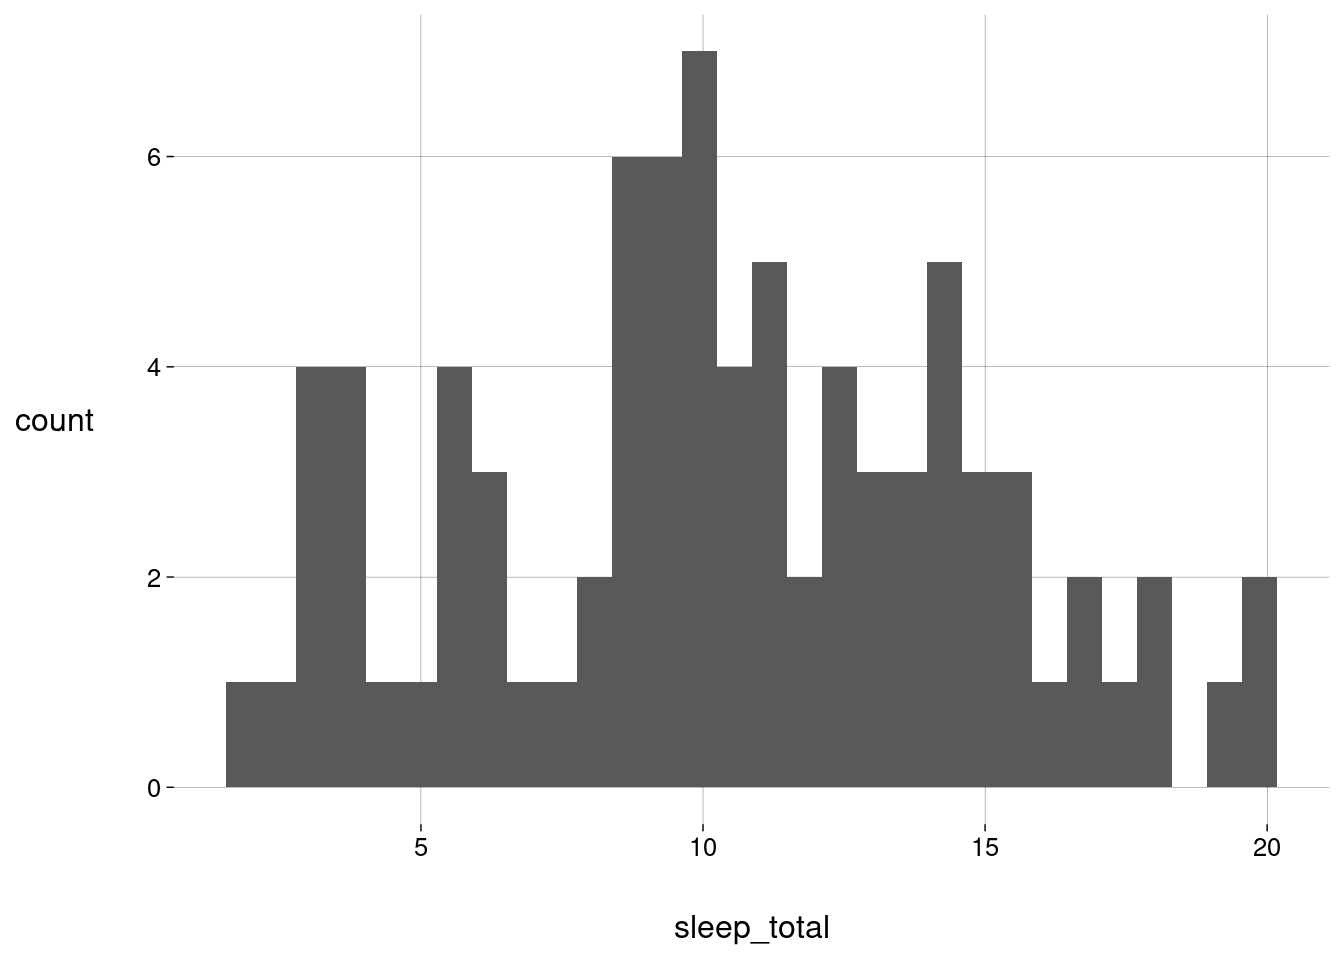
\includegraphics[width=1\linewidth]{_main_files/figure-latex/hist-sono1-1} \end{center}
\item
  \protect\hypertarget{histograma1}{}{} Vamos mudar isto passando um vetor de limites das classes (\emph{breaks}). Vamos acrescentar rótulos também:

\begin{Shaded}
\begin{Highlighting}[]
\NormalTok{sono }\SpecialCharTok{\%\textgreater{}\%} 
  \FunctionTok{ggplot}\NormalTok{(}\FunctionTok{aes}\NormalTok{(}\AttributeTok{x =}\NormalTok{ sleep\_total)) }\SpecialCharTok{+}
    \FunctionTok{geom\_histogram}\NormalTok{(}\AttributeTok{breaks =} \FunctionTok{seq}\NormalTok{(}\DecValTok{0}\NormalTok{, }\DecValTok{20}\NormalTok{, }\DecValTok{2}\NormalTok{)) }\SpecialCharTok{+}
    \FunctionTok{scale\_x\_continuous}\NormalTok{(}\AttributeTok{breaks =} \FunctionTok{seq}\NormalTok{(}\DecValTok{0}\NormalTok{, }\DecValTok{20}\NormalTok{, }\DecValTok{2}\NormalTok{)) }\SpecialCharTok{+}
    \FunctionTok{labs}\NormalTok{(}
      \AttributeTok{title =} \StringTok{\textquotesingle{}Horas de sono de diversos mamíferos\textquotesingle{}}\NormalTok{,}
      \AttributeTok{x =} \StringTok{\textquotesingle{}horas de sono\textquotesingle{}}\NormalTok{,}
      \AttributeTok{y =} \ConstantTok{NULL}\NormalTok{,}
      \AttributeTok{caption =} \StringTok{\textquotesingle{}Fonte: dataset \textasciigrave{}msleep\textasciigrave{}\textquotesingle{}}
\NormalTok{    )}
\end{Highlighting}
\end{Shaded}

  \begin{center}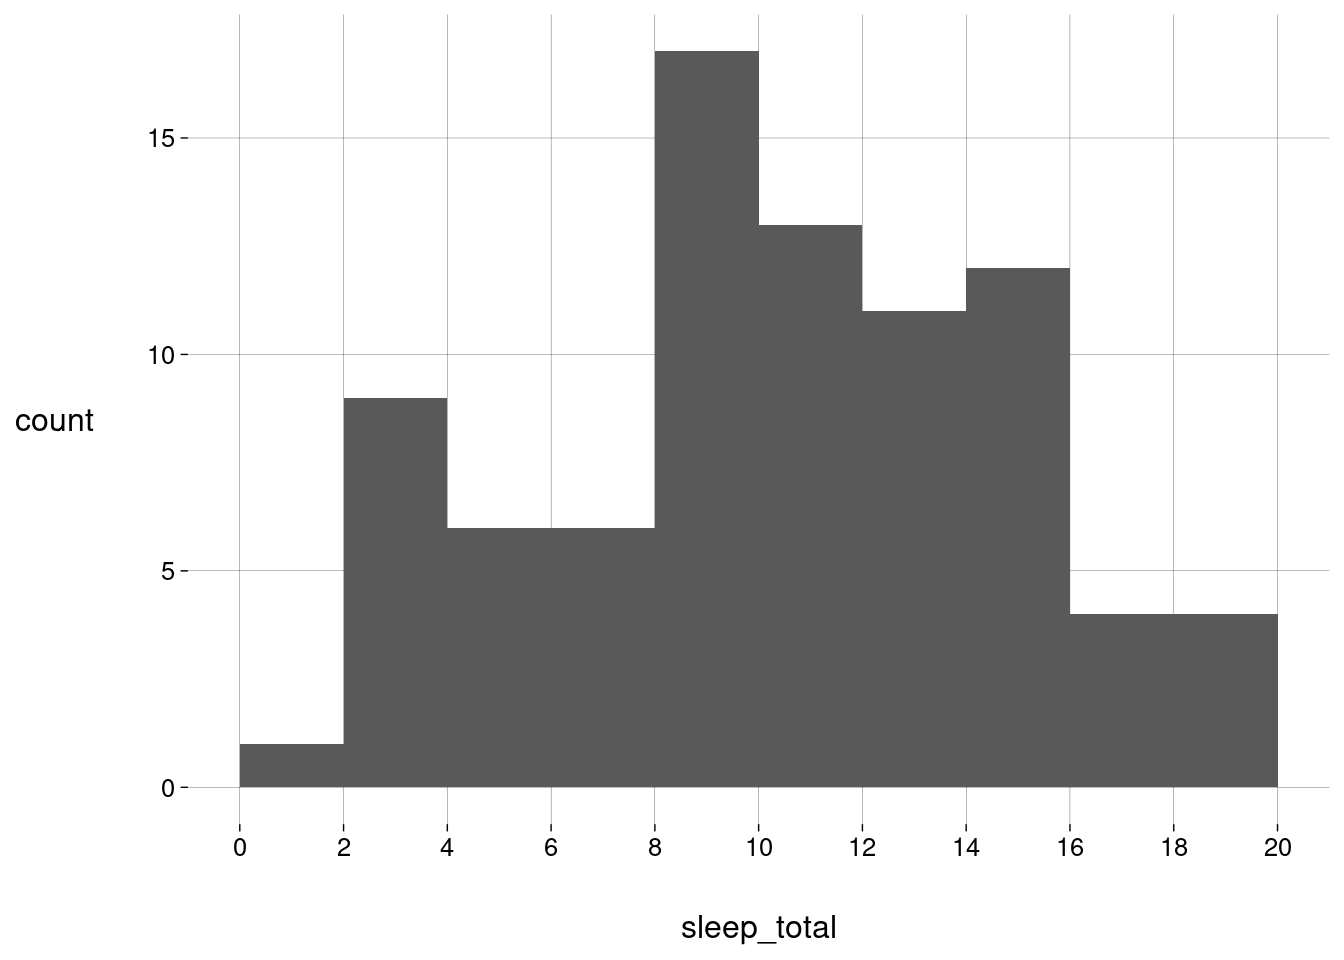
\includegraphics[width=1\linewidth]{_main_files/figure-latex/hist-sono2-1} \end{center}
\item
  Nossas impressões:

  \begin{itemize}
  \item
    A classe que mais tem elementos é a de $8$ a $10$ horas.
  \item
    A distribuição é mais ou menos simétrica.
  \item
    A distribuição tem forma aproximada de sino: há poucos mamíferos com valores extremos de horas de sono; a maioria está próxima do valor médio:

\begin{Shaded}
\begin{Highlighting}[]
\FunctionTok{mean}\NormalTok{(sono}\SpecialCharTok{$}\NormalTok{sleep\_total)}
\DocumentationTok{\#\# [1] 10,43373}
\end{Highlighting}
\end{Shaded}
  \end{itemize}
\end{itemize}

\hypertarget{poluxedgono-de-frequuxeancia}{%
\subsection{Polígono de frequência}\label{poluxedgono-de-frequuxeancia}}

\begin{itemize}
\item
  Em vez das barras do histograma, podemos desenhar uma linha ligando seus topos.
\item
  O resultado é um {\hl{polígono de frequência}}.

\begin{Shaded}
\begin{Highlighting}[]
\NormalTok{pf }\OtherTok{\textless{}{-}}\NormalTok{ sono }\SpecialCharTok{\%\textgreater{}\%} 
  \FunctionTok{ggplot}\NormalTok{(}\FunctionTok{aes}\NormalTok{(}\AttributeTok{x =}\NormalTok{ sleep\_total)) }\SpecialCharTok{+}
    \FunctionTok{geom\_freqpoly}\NormalTok{(}\AttributeTok{breaks =} \FunctionTok{seq}\NormalTok{(}\DecValTok{0}\NormalTok{, }\DecValTok{20}\NormalTok{, }\DecValTok{2}\NormalTok{), }\AttributeTok{color =} \StringTok{\textquotesingle{}red\textquotesingle{}}\NormalTok{) }\SpecialCharTok{+}
    \FunctionTok{scale\_x\_continuous}\NormalTok{(}\AttributeTok{breaks =} \FunctionTok{seq}\NormalTok{(}\DecValTok{0}\NormalTok{, }\DecValTok{20}\NormalTok{, }\DecValTok{2}\NormalTok{))}

\NormalTok{pf}
\end{Highlighting}
\end{Shaded}

  \begin{center}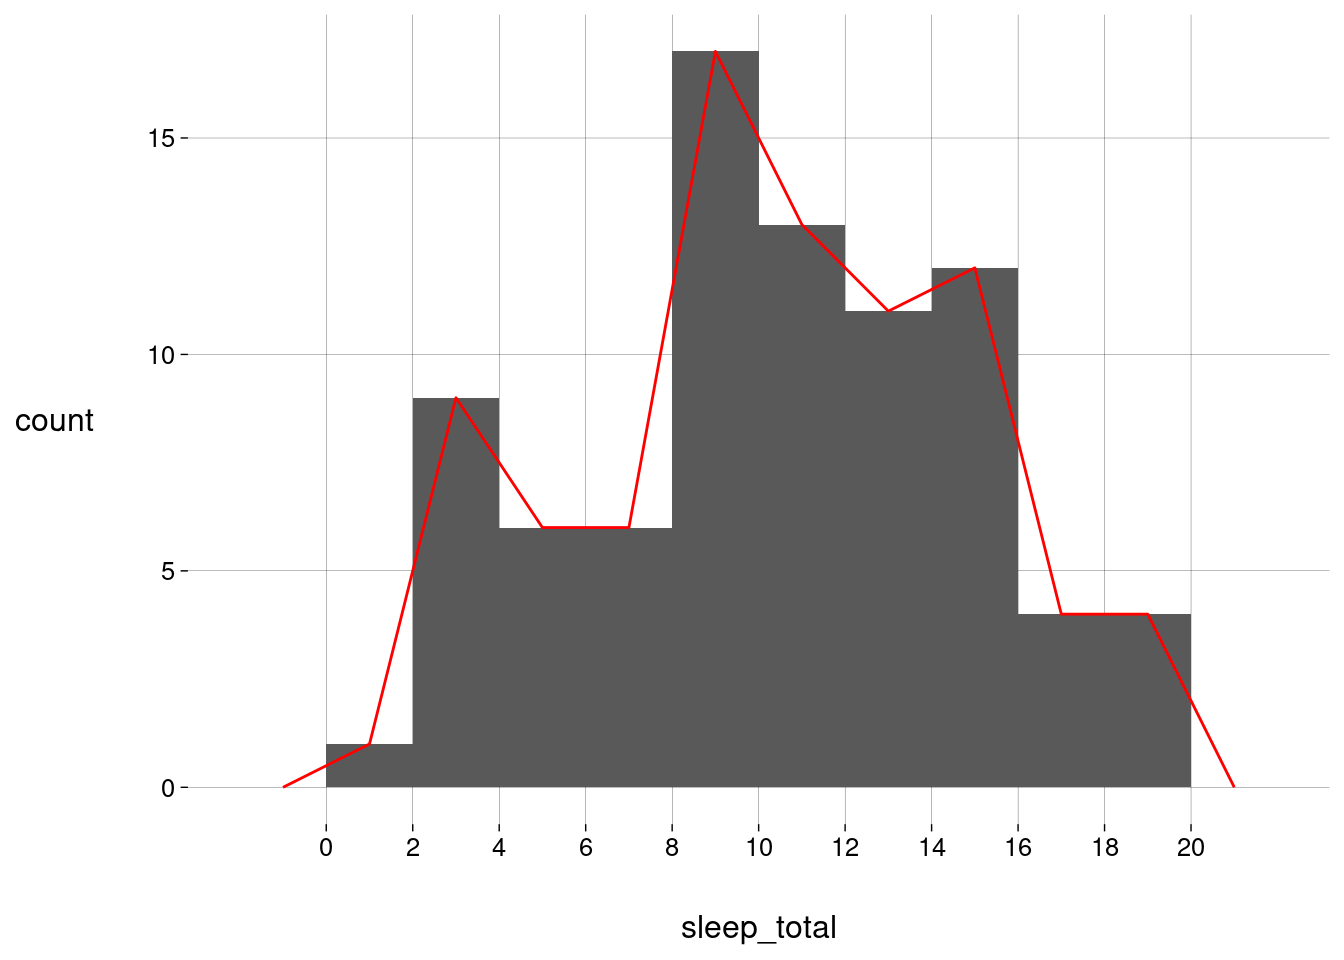
\includegraphics[width=1\linewidth]{_main_files/figure-latex/hist-freqpoly-1} \end{center}
\item
  Vamos sobrepor o polígono de frequência ao histograma, para deixar claro o que está acontecendo:

\begin{Shaded}
\begin{Highlighting}[]
\NormalTok{pf }\SpecialCharTok{+} \FunctionTok{geom\_histogram}\NormalTok{(}\AttributeTok{breaks =} \FunctionTok{seq}\NormalTok{(}\DecValTok{0}\NormalTok{, }\DecValTok{20}\NormalTok{, }\DecValTok{2}\NormalTok{), }\AttributeTok{alpha =}\NormalTok{ .}\DecValTok{3}\NormalTok{)}
\end{Highlighting}
\end{Shaded}

  \begin{center}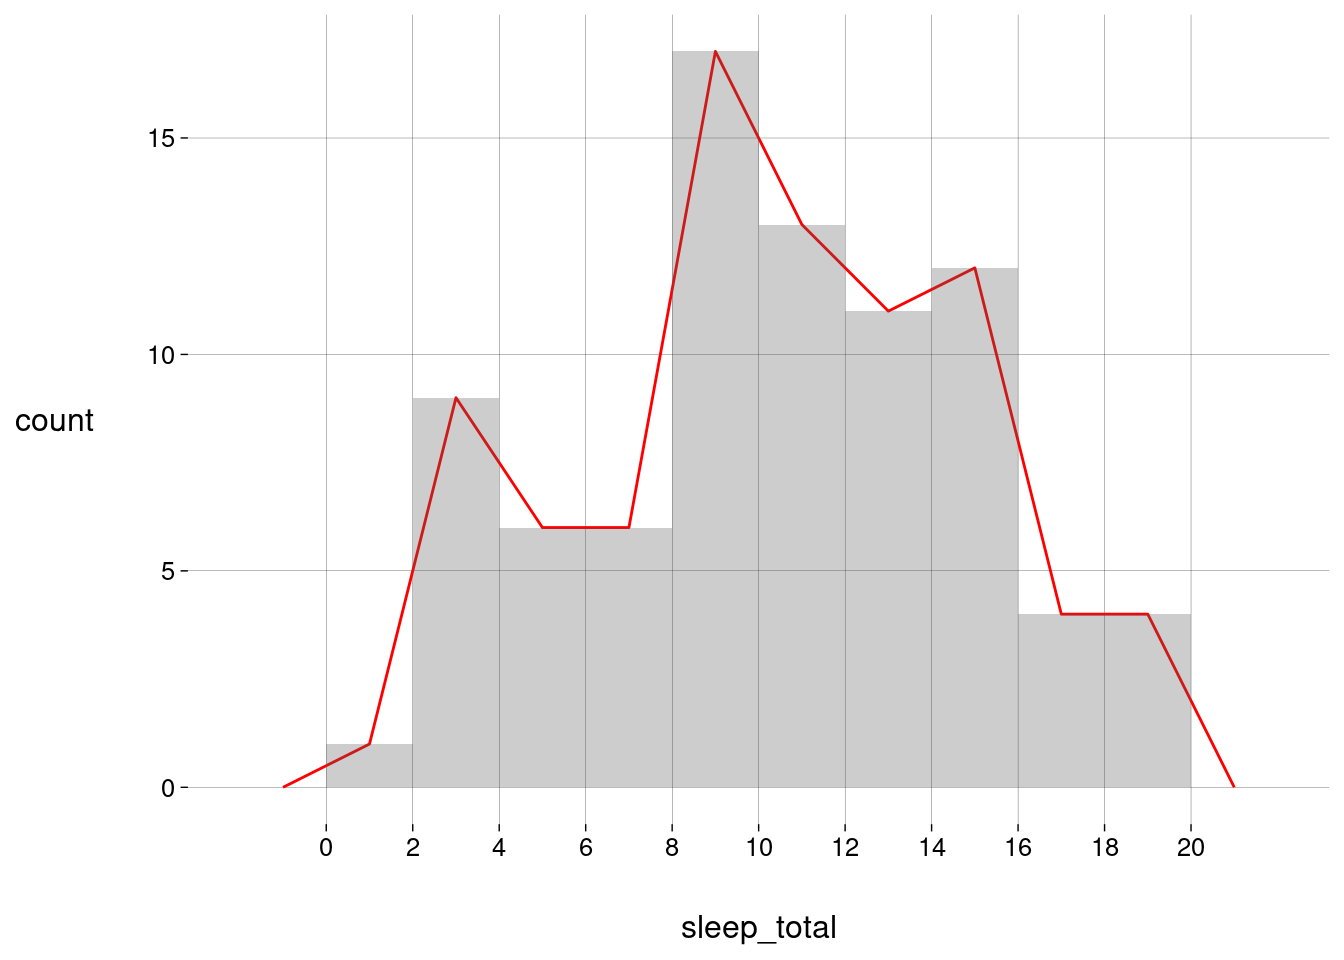
\includegraphics[width=1\linewidth]{_main_files/figure-latex/hist-freqpoly2-1} \end{center}
\end{itemize}

\hypertarget{ogiva}{%
\section{Ogiva}\label{ogiva}}

\begin{itemize}
\item
  A ogiva é um gráfico que mostra a {\hl{frequência acumulada}}: para cada valor $v$ da variável no eixo $x$, a proporção de indivíduos com valor menor ou igual a $v$.
\item
  A geometria \texttt{geom\_step} gera o gráfico de uma {\hl{função degrau}}.
\item
  Cada geometria está ligada a uma {\hl{\texttt{stat}}}, um algoritmo para computar o que vai ser desenhado. Aqui, passamos para a geometria {\hl{a função \texttt{ecdf} (\emph{empirical cumulative distribution function}), do pacote \texttt{stats}, que calcula as frequências acumuladas.}}

\begin{Shaded}
\begin{Highlighting}[]
\NormalTok{sono }\SpecialCharTok{\%\textgreater{}\%} 
  \FunctionTok{ggplot}\NormalTok{(}\FunctionTok{aes}\NormalTok{(}\AttributeTok{x =}\NormalTok{ sleep\_total)) }\SpecialCharTok{+}
    \FunctionTok{geom\_step}\NormalTok{(}\AttributeTok{stat =} \StringTok{\textquotesingle{}ecdf\textquotesingle{}}\NormalTok{) }\SpecialCharTok{+}
    \FunctionTok{scale\_x\_continuous}\NormalTok{(}\AttributeTok{breaks =} \FunctionTok{seq}\NormalTok{(}\DecValTok{0}\NormalTok{, }\DecValTok{20}\NormalTok{, }\DecValTok{2}\NormalTok{)) }\SpecialCharTok{+}
    \FunctionTok{scale\_y\_continuous}\NormalTok{(}\AttributeTok{breaks =} \FunctionTok{seq}\NormalTok{(}\DecValTok{0}\NormalTok{, }\DecValTok{1}\NormalTok{, .}\DecValTok{1}\NormalTok{)) }\SpecialCharTok{+}
    \FunctionTok{labs}\NormalTok{(}\AttributeTok{y =} \ConstantTok{NULL}\NormalTok{)}
\end{Highlighting}
\end{Shaded}

  \begin{center}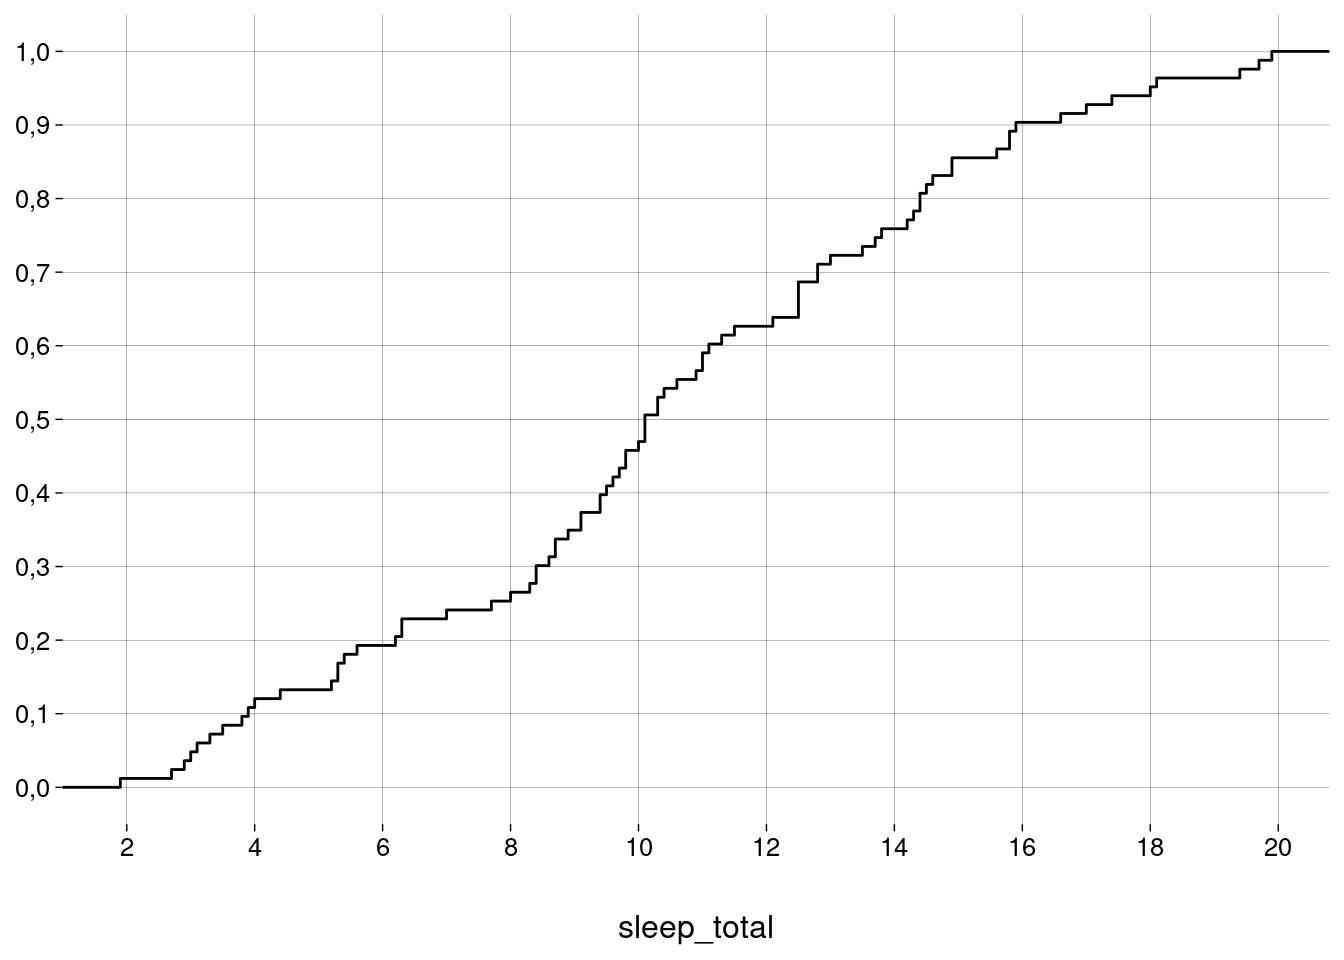
\includegraphics[width=1\linewidth]{_main_files/figure-latex/ogiva-1} \end{center}
\item
  Com a ogiva, podemos obter informações difíceis de visualizar no histograma. Por exemplo:

  \begin{itemize}
  \item
    Cerca de $20\%$ dos mamíferos têm menos de $6$ horas de sono.
  \item
    Cerca de metade dos mamíferos têm menos de $10$ horas de sono.
  \item
    Cerca de $10\%$ dos mamíferos têm mais de $16$ horas de sono.
  \end{itemize}
\end{itemize}

\hypertarget{ramos-e-folhas}{%
\section{Ramos e folhas}\label{ramos-e-folhas}}

\begin{itemize}
\item
  No início dos anos $1900$, quando estatísticas eram feitas à mão, Arthur Bowley criou os {\hl{diagramas de ramos e folhas}}.
\item
  Um diagrama de ramos e folhas é, basicamente, uma listagem de todos os valores de uma variável, agrupados de maneira que todos os valores de uma classe (i.e., de uma linha) têm os algarismos iniciais dentro de um intervalo.
\item
  Para as horas de sono dos mamíferos:

\begin{Shaded}
\begin{Highlighting}[]
\NormalTok{sono}\SpecialCharTok{$}\NormalTok{sleep\_total }\SpecialCharTok{\%\textgreater{}\%} 
  \FunctionTok{stem}\NormalTok{()}
\DocumentationTok{\#\# }
\DocumentationTok{\#\#   The decimal point is at the |}
\DocumentationTok{\#\# }
\DocumentationTok{\#\#    0 | 9}
\DocumentationTok{\#\#    2 | 79013589}
\DocumentationTok{\#\#    4 | 0423346}
\DocumentationTok{\#\#    6 | 23307}
\DocumentationTok{\#\#    8 | 03446779114456788}
\DocumentationTok{\#\#   10 | 01113346900135}
\DocumentationTok{\#\#   12 | 15555880578}
\DocumentationTok{\#\#   14 | 234456996889}
\DocumentationTok{\#\#   16 | 604}
\DocumentationTok{\#\#   18 | 01479}
\end{Highlighting}
\end{Shaded}
\item
  A primeira linha representa um indivíduo com $0{,}9$ horas de sono.
\item
  A penúltima linha representa $3$ valores:

  \begin{itemize}
  \tightlist
  \item
    $16{,}6$
  \item
    $17{,}0$
  \item
    $17{,}4$
  \end{itemize}
\end{itemize}

\hypertarget{personalizauxe7uxe3o-do-tema}{%
\section{Personalização do tema}\label{personalizauxe7uxe3o-do-tema}}

\begin{itemize}
\item
  O \texttt{ggplot2} tem um tema \emph{default}, chamado \texttt{theme\_gray}, que gera \protect\hyperlink{grafico4}{o \emph{scatterplot} de um exemplo anterior} deste capítulo do seguinte modo:

  \begin{center}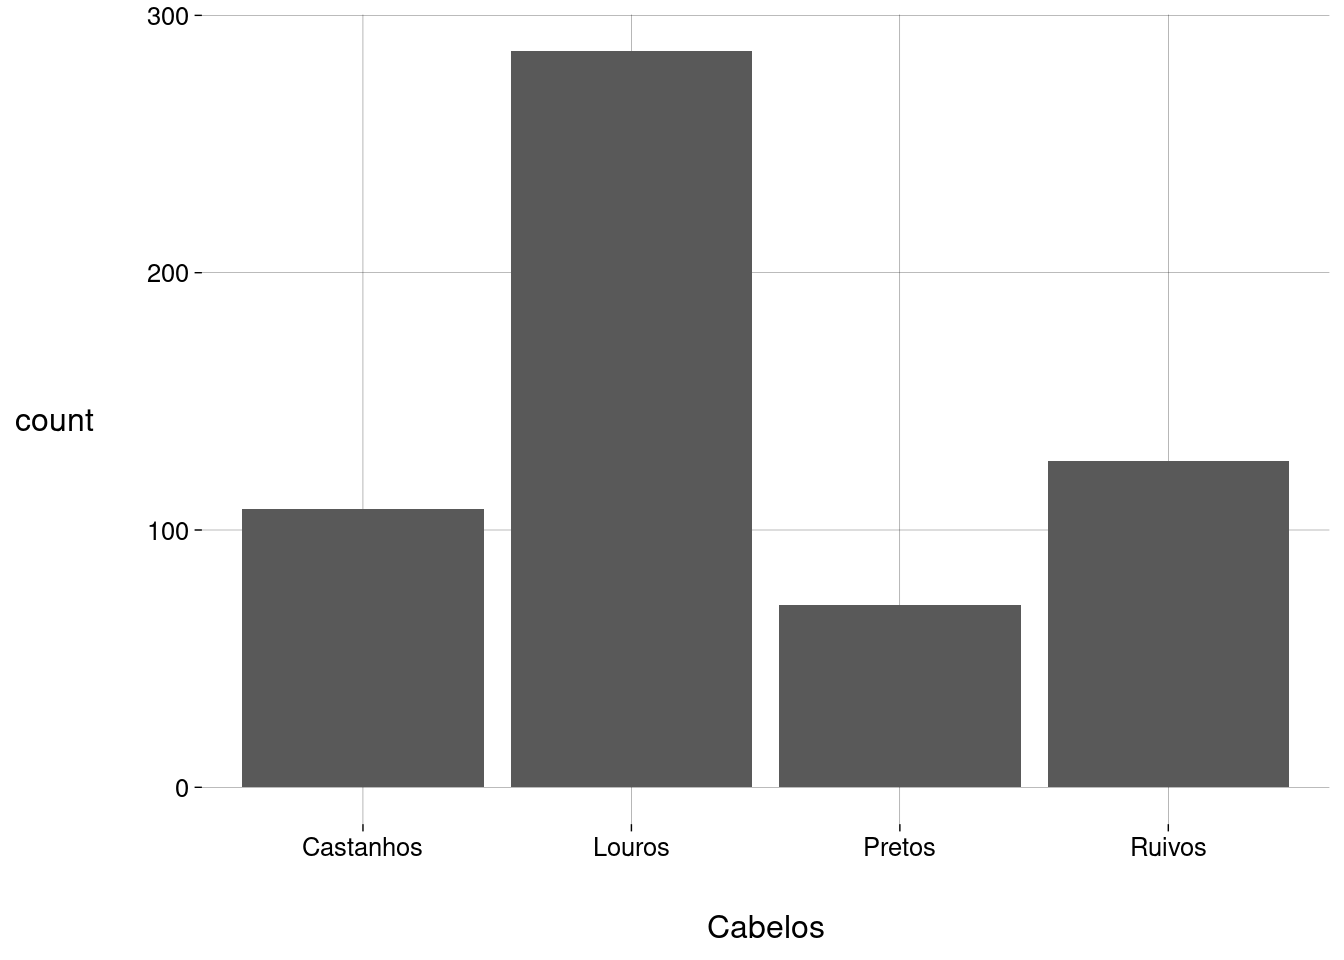
\includegraphics[width=1\linewidth]{_main_files/figure-latex/unnamed-chunk-26-1} \end{center}
\item
  Para este material, escolhi o tema \texttt{theme\_linedraw}, que usa linhas pretas sobre fundo branco:

  \begin{center}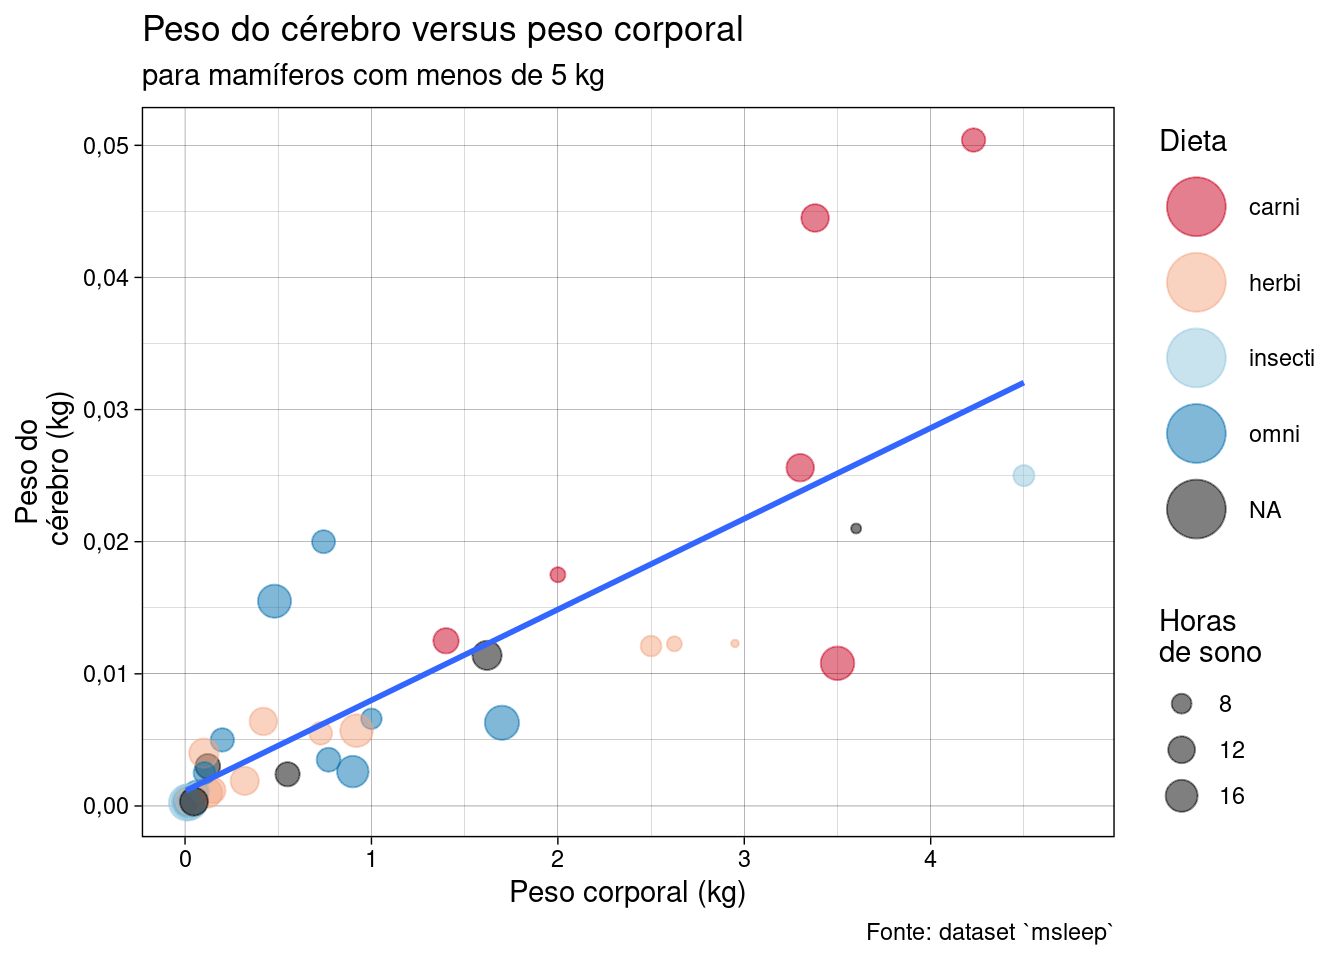
\includegraphics[width=1\linewidth]{_main_files/figure-latex/unnamed-chunk-27-1} \end{center}
\item
  Para deixar os gráficos mais leves e facilitar a leitura, fiz as seguintes alterações no tema:

  \begin{itemize}
  \item
    Mudei o tamanho do texto dos rótulos.
  \item
    Fiz o rótulo do eixo $y$ aparecer na horizontal; embora isto ocupe um pouco mais de espaço, evita que o leitor tenha que girar a cabeça para ler o rótulo.
  \item
    Eliminei as linhas dos eixos, para o gráfico ficar mais leve.
  \item
    Eliminei a moldura da área de dados, para o gráfico ficar mais leve.
  \item
    Eliminei a grade secundária, para o gráfico ficar mais leve.
  \end{itemize}
\item
  O resultado é

  \begin{center}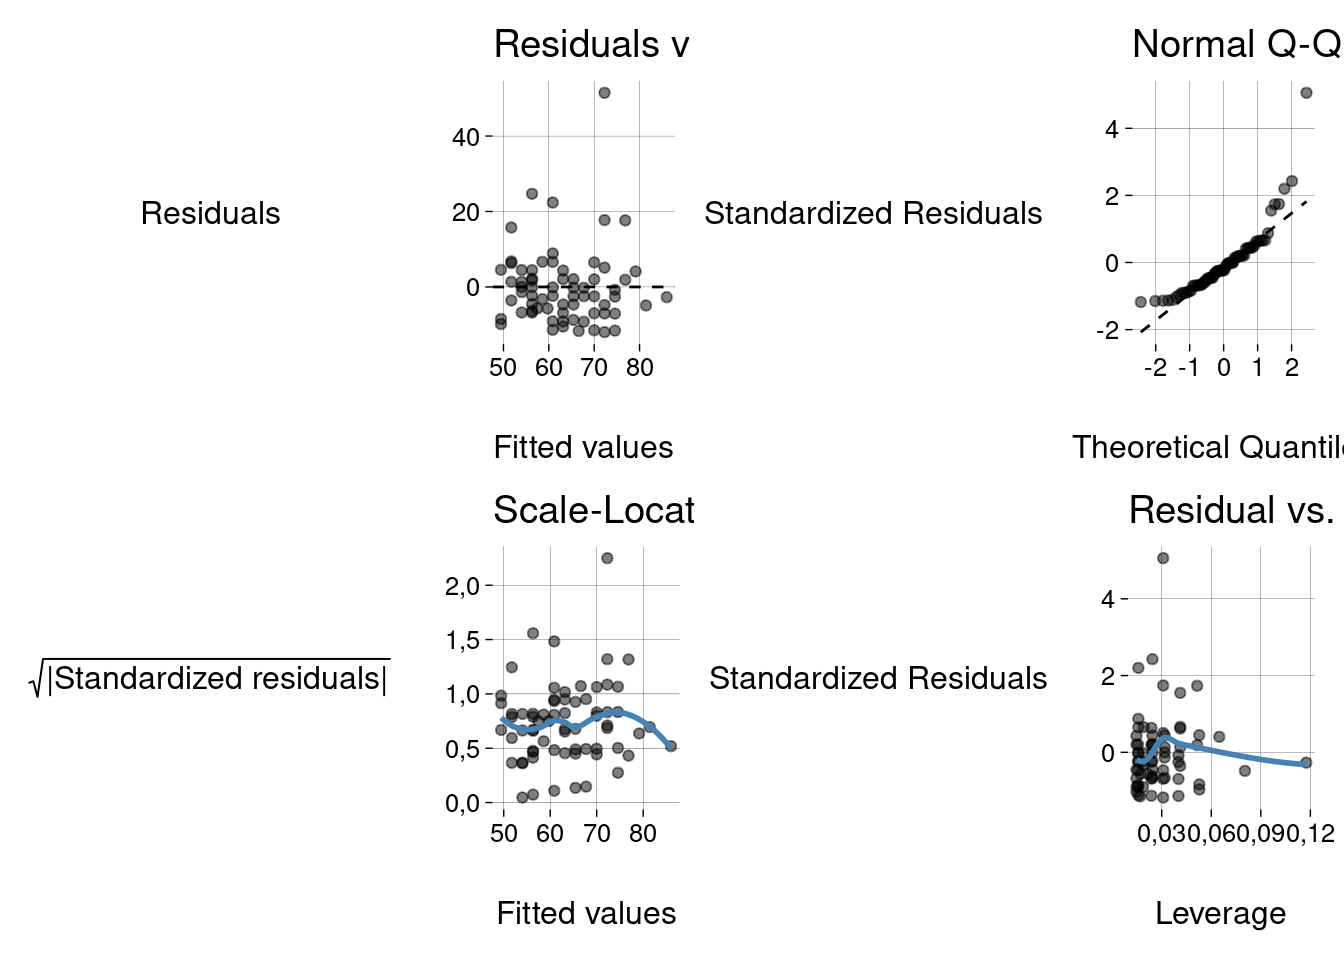
\includegraphics[width=1\linewidth]{_main_files/figure-latex/unnamed-chunk-28-1} \end{center}
\item
  Os meus comandos para alterar o tema são

\begin{Shaded}
\begin{Highlighting}[]
\CommentTok{\# Tamanho do texto depende do formato de saída (html ou pdf):}
\NormalTok{plot\_text\_size }\OtherTok{=} \FunctionTok{ifelse}\NormalTok{(}\FunctionTok{is\_html\_output}\NormalTok{(), }\DecValTok{12}\NormalTok{, }\DecValTok{13}\NormalTok{)}

\CommentTok{\# Tema mais leve:}
\FunctionTok{theme\_set}\NormalTok{(}
  \FunctionTok{theme\_linedraw}\NormalTok{() }\SpecialCharTok{+}
    \FunctionTok{theme}\NormalTok{(}
      \CommentTok{\# Tamanho do texto}
      \AttributeTok{text =} \FunctionTok{element\_text}\NormalTok{(}\AttributeTok{size =}\NormalTok{ plot\_text\_size),}
      \CommentTok{\# Eixo y}
      \AttributeTok{axis.title.y.left =} \FunctionTok{element\_text}\NormalTok{(}
        \CommentTok{\# Nunca girar o rótulo do eixo y}
        \AttributeTok{angle =} \DecValTok{0}\NormalTok{,}
        \CommentTok{\# Separar o rótulo do eixo um pouco}
        \AttributeTok{margin =} \FunctionTok{margin}\NormalTok{(}\AttributeTok{r =} \DecValTok{20}\NormalTok{),}
        \CommentTok{\# Posicionar verticalmente no meio}
        \AttributeTok{vjust =}\NormalTok{ .}\DecValTok{5}
\NormalTok{      ),}
      \CommentTok{\# Eixo y secundário (à direita), quando presente}
      \AttributeTok{axis.title.y.right =} \FunctionTok{element\_text}\NormalTok{(}
        \CommentTok{\# Nunca girar o rótulo do eixo y}
        \AttributeTok{angle =} \DecValTok{0}\NormalTok{,}
        \CommentTok{\# Separar o rótulo do eixo um pouco}
        \AttributeTok{margin =} \FunctionTok{margin}\NormalTok{(}\AttributeTok{l =} \DecValTok{20}\NormalTok{),}
        \CommentTok{\# Posicionar verticalmente no meio}
        \AttributeTok{vjust =}\NormalTok{ .}\DecValTok{5}
\NormalTok{      ),}
      \CommentTok{\# Não colocar marcas no eixo y secundário}
      \AttributeTok{axis.ticks.y.right =} \FunctionTok{element\_blank}\NormalTok{(),}
      \CommentTok{\# Separar o eixo x do rótulo um pouco mais}
      \AttributeTok{axis.title.x.bottom =} \FunctionTok{element\_text}\NormalTok{(}
        \AttributeTok{margin =} \FunctionTok{margin}\NormalTok{(}\AttributeTok{t =} \DecValTok{20}\NormalTok{)}
\NormalTok{      ),}
      \CommentTok{\# Eliminar linhas dos eixos}
      \AttributeTok{axis.line =} \FunctionTok{element\_blank}\NormalTok{(),}
      \CommentTok{\# Eliminar a moldura da área de dados}
      \AttributeTok{panel.border =} \FunctionTok{element\_blank}\NormalTok{(),}
      \CommentTok{\# Eliminar a grade secundária}
      \AttributeTok{panel.grid.minor =} \FunctionTok{element\_blank}\NormalTok{()}
\NormalTok{    )}
\NormalTok{)}
\end{Highlighting}
\end{Shaded}
\end{itemize}

\hypertarget{exercuxedcios-3}{%
\section{Exercícios}\label{exercuxedcios-3}}

\begin{rmdimportant}
Não se esqueça de incluir títulos nos gráficos e rótulos nos eixos.

\end{rmdimportant}

\hypertarget{peso-cerebral-e-peso-corporal}{%
\subsection{Peso cerebral e peso corporal}\label{peso-cerebral-e-peso-corporal}}

\begin{enumerate}
\def\labelenumi{\arabic{enumi}.}
\item
  Observe os \protect\hyperlink{grafico4}{comandos que geraram o gráfico \texttt{grafico4}}.
\item
  O que acontece se você retirar \texttt{aes(group\ =\ 1)} da chamada a \texttt{geom\_smooth}? Explique.
\item
  O que acontece se você mudar \texttt{show.legend\ =\ FALSE} para \texttt{show.legend\ =\ TRUE} na chamada a \texttt{geom\_smooth}? Explique.
\item
  O que acontece se você mudar \texttt{se\ =\ FALSE} para \texttt{se\ =\ TRUE} na chamada a \texttt{geom\_smooth}? Explique.
\item
  Acrescente ao gráfico a camada \texttt{facet\_wrap(\textasciitilde{}vore)}. O que acontece?
\item
  Examine o \emph{data frame} \texttt{sono} e identifique o único insetívoro com mais de $4$kg.
\item
  Instale o pacote \texttt{gg\_repel} e acrescente ao gráfico \texttt{grafico4} (não facetado) a geometria \texttt{geom\_label\_repel} (consulte a ajuda) para rotular o mamífero insetívoro identificado no item anterior com o seu nome, {\hl{sem cobrir outros pontos do gráfico}}. Cuidado para não alterar a legenda que já existe.
\end{enumerate}

\hypertarget{peso-cerebral-e-horas-de-sono}{%
\subsection{Peso cerebral e horas de sono}\label{peso-cerebral-e-horas-de-sono}}

\begin{rmdbox}

Use o \emph{data frame} \texttt{sono} definido como

\begin{Shaded}
\begin{Highlighting}[]
\FunctionTok{library}\NormalTok{(ggplot2)}

\NormalTok{sono }\OtherTok{\textless{}{-}}\NormalTok{ msleep }\SpecialCharTok{\%\textgreater{}\%} 
  \FunctionTok{select}\NormalTok{(}
\NormalTok{    name, order, genus, vore, bodywt, }
\NormalTok{    brainwt, awake, sleep\_total}
\NormalTok{  )}
\end{Highlighting}
\end{Shaded}

\end{rmdbox}

\begin{enumerate}
\def\labelenumi{\arabic{enumi}.}
\item
  Construa um histograma da variável \texttt{brainwt}. Escolha o número de classes que você achar melhor. O que acontece com os valores \texttt{NA}?
\item
  \href{http://sillasgonzaga.com/material/curso_visualizacao/ggplot2-parte-ii.html\#customizando-escalas}{Descubra que função da forma \texttt{scale\_x\_...} usar} para fazer com que o eixo $x$ tenha uma escala logarítmica. Gere um novo histograma.
\item
  Qual dos dois histogramas é melhor para responder a pergunta ``\emph{Qual a faixa de peso cerebral que tem mais animais?}'' de forma satisfatória?
\item
  Construa um \emph{scatter plot} de horas de sono versus peso do cérebro. Você percebe alguma correlação entre estas variáveis? Se precisar, concentre-se em um subconjunto dos dados.
\item
  Usando \texttt{geom\_smooth} (\href{https://cdr.ibpad.com.br/ggplot2.html\#objetos-geom\%C3\%A9tricos-e-tipos-de-gr\%C3\%A1ficos}{leia a respeito}), sobreponha uma reta de regressão ao gráfico de dispersão, usando o método \texttt{lm} e sem o erro padrão (i.e., com \texttt{se\ =\ FALSE}). O que você observa? Discuta.
\end{enumerate}

\hypertarget{igualdade-de-guxeanero-entre-furacuxf5es}{%
\subsection{Igualdade de gênero entre furacões?}\label{igualdade-de-guxeanero-entre-furacuxf5es}}

\href{https://www.pnas.org/content/111/24/8782}{Este artigo} tenta achar uma relação entre o gênero do nome de um furacão e a quantidade de vítimas fatais provocadas por ele.

\begin{rmdbox}

Os dados estão no pacote \texttt{DAAG}, que deve ser instalado:

\begin{Shaded}
\begin{Highlighting}[]
\ControlFlowTok{if}\NormalTok{ (}\SpecialCharTok{!}\FunctionTok{require}\NormalTok{(DAAG))}
  \FunctionTok{install.packages}\NormalTok{(}\StringTok{"DAAG"}\NormalTok{)}
\end{Highlighting}
\end{Shaded}

Vamos usar apenas algumas das variáveis, com nomes em português.

\begin{Shaded}
\begin{Highlighting}[]
\NormalTok{df }\OtherTok{\textless{}{-}}\NormalTok{ hurricNamed }\SpecialCharTok{\%\textgreater{}\%} 
  \FunctionTok{as\_tibble}\NormalTok{() }\SpecialCharTok{\%\textgreater{}\%} 
  \FunctionTok{transmute}\NormalTok{(}
    \AttributeTok{id =} \FunctionTok{paste}\NormalTok{(Year, Name, }\AttributeTok{sep =} \StringTok{\textquotesingle{}{-}\textquotesingle{}}\NormalTok{),}
    \AttributeTok{nome =}\NormalTok{ Name,}
    \AttributeTok{ano =}\NormalTok{ Year,}
    \AttributeTok{velocidade =}\NormalTok{ LF.WindsMPH }\SpecialCharTok{*} \FloatTok{1.8}\NormalTok{,     }\CommentTok{\# convertido para km/h}
    \AttributeTok{pressao =}\NormalTok{ LF.PressureMB,            }\CommentTok{\# mbar}
    \AttributeTok{prejuizo =}\NormalTok{ BaseDam2014 }\SpecialCharTok{\%\textgreater{}\%} \FunctionTok{round}\NormalTok{(), }\CommentTok{\# milhões de dólares de 2014}
    \AttributeTok{mortes =}\NormalTok{ deaths,}
    \AttributeTok{genero =}\NormalTok{ mf}
\NormalTok{  )}
\end{Highlighting}
\end{Shaded}

\end{rmdbox}

\begin{enumerate}
\def\labelenumi{\arabic{enumi}.}
\item
  Crie histogramas para as seguintes variáveis, escolhendo a quantidade de barras que você achar melhor.

  \begin{itemize}
  \item
    \texttt{velocidade}
  \item
    \texttt{prejuizo}
  \item
    \texttt{mortes}
  \end{itemize}

  Não se esqueça de incluir títulos nos gráficos e rótulos nos eixos.

  Comente os histogramas.
\item
  Os histogramas de prejuízos e mortes não ficaram bons. Vamos gerar histogramas transformados.

  No \emph{data frame}, crie duas novas colunas:

  \begin{itemize}
  \item
    \texttt{logprejuizo}: \emph{logaritmo} do prejuízo (na base $10$)
  \item
    \texttt{logmortes}: \emph{logaritmo} do número de mortes (na base $10$)
  \end{itemize}

  Agora, gere histogramas destas duas novas variáveis.
\item
  O que significa o valor do logaritmo do prejuízo na base $10$?
\item
  O que significa o valor do logaritmo do número de mortes na base $10$?
\item
  Por que o histograma do logaritmo do número de mortes vem com uma mensagem de aviso?
\item
  Por que isto não acontece com o logaritmo do prejuízo?
\item
  Faça um gráfico de dispersão com \texttt{pressao} no eixo $y$ e \texttt{velocidade} no eixo $x$.
\item
  Usando \texttt{geom\_smooth} (\href{https://cdr.ibpad.com.br/ggplot2.html\#objetos-geom\%C3\%A9tricos-e-tipos-de-gr\%C3\%A1ficos}{leia a respeito}), sobreponha uma reta de regressão ao gráfico, usando o método \texttt{lm} e sem o erro padrão (i.e., com \texttt{se\ =\ FALSE}). O que você observa? Discuta.
\item
  Faça um gráfico de dispersão com \texttt{logmortes} no eixo $y$ e \texttt{pressao} no eixo $x$.
\item
  Usando \texttt{geom\_smooth} (\href{https://cdr.ibpad.com.br/ggplot2.html\#objetos-geom\%C3\%A9tricos-e-tipos-de-gr\%C3\%A1ficos}{leia a respeito}), sobreponha uma reta de regressão ao gráfico, usando o método \texttt{lm} e sem o erro padrão (i.e., com \texttt{se\ =\ FALSE}). O que você observa? Discuta.
\item
  Faça um gráfico de dispersão com \texttt{logmortes} no eixo $y$ e \texttt{pressao} no eixo $x$, com pontos coloridos de acordo com o gênero do nome do furacão.
\item
  Usando \texttt{geom\_smooth} (\href{https://cdr.ibpad.com.br/ggplot2.html\#objetos-geom\%C3\%A9tricos-e-tipos-de-gr\%C3\%A1ficos}{leia a respeito}), sobreponha retas de regressão ao gráfico, uma para cada gênero, usando o método \texttt{lm} e sem o erro padrão (i.e., com \texttt{se\ =\ FALSE}). O que você observa? Discuta.
\end{enumerate}

\begin{rmdcaution}
Visualizações como esta ajudam a explorar os dados, mas não servem para testar rigorosamente a hipótese de que furacões mulheres matam mais do que furacões homens.

Mais adiante no curso, vamos aprender a fazer testes mais rigorosos sobre hipóteses como esta.

\end{rmdcaution}

\hypertarget{viz2}{%
\chapter{Visualização com ggplot2 (continuação)}\label{viz2}}

\begin{rmdtip}
Busque mais informações sobre os pacotes \texttt{tidyverse} e \texttt{ggplot2} \protect\hyperlink{refrec}{nas referências recomendadas}.

\end{rmdtip}

\hypertarget{vuxeddeo-1-3}{%
\section{Vídeo 1}\label{vuxeddeo-1-3}}

\begin{center} \url{https://youtu.be/TjgLDeIQHIc} \end{center}

\hypertarget{boxplots}{%
\section{\texorpdfstring{\emph{Boxplots}}{Boxplots}}\label{boxplots}}

\hypertarget{conjunto-de-dados-1}{%
\subsection{Conjunto de dados}\label{conjunto-de-dados-1}}

\begin{itemize}
\item
  Vamos continuar a trabalhar com os dados sobre as horas de sono de alguns mamíferos:

\begin{Shaded}
\begin{Highlighting}[]
\NormalTok{sono }\OtherTok{\textless{}{-}}\NormalTok{ msleep }\SpecialCharTok{\%\textgreater{}\%} 
  \FunctionTok{select}\NormalTok{(name, vore, order, sleep\_total)}

\NormalTok{sono}
\DocumentationTok{\#\# \# A tibble: 83 x 4}
\DocumentationTok{\#\#   name                       vore  order        sleep\_total}
\DocumentationTok{\#\#   \textless{}chr\textgreater{}                      \textless{}chr\textgreater{} \textless{}chr\textgreater{}              \textless{}dbl\textgreater{}}
\DocumentationTok{\#\# 1 Cheetah                    carni Carnivora           12.1}
\DocumentationTok{\#\# 2 Owl monkey                 omni  Primates            17  }
\DocumentationTok{\#\# 3 Mountain beaver            herbi Rodentia            14.4}
\DocumentationTok{\#\# 4 Greater short{-}tailed shrew omni  Soricomorpha        14.9}
\DocumentationTok{\#\# 5 Cow                        herbi Artiodactyla         4  }
\DocumentationTok{\#\# 6 Three{-}toed sloth           herbi Pilosa              14.4}
\DocumentationTok{\#\# \# ... with 77 more rows}
\end{Highlighting}
\end{Shaded}
\end{itemize}

\hypertarget{mediana-e-quartis}{%
\subsection{Mediana e quartis}\label{mediana-e-quartis}}

\begin{itemize}
\item
  Para entender \emph{boxplots}, precisamos, antes, entender algumas medidas.
\item
  Se tomarmos as quantidades de horas de sono de todos os animais do conjunto de dados e {\hl{classificarmos estas quantidades em ordem crescente}}, vamos ter:

\begin{Shaded}
\begin{Highlighting}[]
\NormalTok{horas }\OtherTok{\textless{}{-}}\NormalTok{ sono }\SpecialCharTok{\%\textgreater{}\%} 
  \FunctionTok{pull}\NormalTok{(sleep\_total) }\SpecialCharTok{\%\textgreater{}\%} 
  \FunctionTok{sort}\NormalTok{()}

\NormalTok{horas}
\DocumentationTok{\#\#  [1]  1,9  2,7  2,9  3,0  3,1  3,3  3,5  3,8  3,9  4,0  4,4  5,2  5,3}
\DocumentationTok{\#\# [14]  5,3  5,4  5,6  6,2  6,3  6,3  7,0  7,7  8,0  8,3  8,4  8,4  8,6}
\DocumentationTok{\#\# [27]  8,7  8,7  8,9  9,1  9,1  9,4  9,4  9,5  9,6  9,7  9,8  9,8 10,0}
\DocumentationTok{\#\# [40] 10,1 10,1 10,1 10,3 10,3 10,4 10,6 10,9 11,0 11,0 11,1 11,3 11,5}
\DocumentationTok{\#\# [53] 12,1 12,5 12,5 12,5 12,5 12,8 12,8 13,0 13,5 13,7 13,8 14,2 14,3}
\DocumentationTok{\#\# [66] 14,4 14,4 14,5 14,6 14,9 14,9 15,6 15,8 15,8 15,9 16,6 17,0 17,4}
\DocumentationTok{\#\# [79] 18,0 18,1 19,4 19,7 19,9}
\end{Highlighting}
\end{Shaded}
\item
  Quantos valores são?

\begin{Shaded}
\begin{Highlighting}[]
\FunctionTok{length}\NormalTok{(horas)}
\DocumentationTok{\#\# [1] 83}
\end{Highlighting}
\end{Shaded}
\item
  O valor que está {\hl{bem no meio desta fila}} --- i.e., na posição $42$ --- é a {\hl{mediana}}:

\begin{Shaded}
\begin{Highlighting}[]
\NormalTok{horas[}\FunctionTok{ceiling}\NormalTok{(}\FunctionTok{length}\NormalTok{(horas) }\SpecialCharTok{/} \DecValTok{2}\NormalTok{)]}
\DocumentationTok{\#\# [1] 10,1}
\end{Highlighting}
\end{Shaded}
\item
  Em R:

\begin{Shaded}
\begin{Highlighting}[]
\FunctionTok{median}\NormalTok{(horas)}
\DocumentationTok{\#\# [1] 10,1}
\end{Highlighting}
\end{Shaded}

  \begin{rmdcaution}
  Mediana e média são coisas muito diferentes.

  Por acaso, neste exemplo, a média das horas é próxima da mediana:

\begin{Shaded}
\begin{Highlighting}[]
\FunctionTok{mean}\NormalTok{(horas)}
\DocumentationTok{\#\# [1] 10,43373}
\end{Highlighting}
\end{Shaded}

  Isto costuma acontecer quando a distribuição dos dados é aproximadamente simétrica.

  \end{rmdcaution}
\item
  Os {\hl{quartis}} são os valores que estão nas posições $\frac14$, $\frac12$ e $\frac34$ da fila. São o {\hl{primeiro, segundo e terceiro quartis}}, respectivamente.

\begin{Shaded}
\begin{Highlighting}[]
\NormalTok{horas[}
  \FunctionTok{c}\NormalTok{(}
    \FunctionTok{ceiling}\NormalTok{(}\FunctionTok{length}\NormalTok{(horas) }\SpecialCharTok{/} \DecValTok{4}\NormalTok{),}
    \FunctionTok{ceiling}\NormalTok{(}\FunctionTok{length}\NormalTok{(horas) }\SpecialCharTok{/} \DecValTok{2}\NormalTok{),}
    \FunctionTok{ceiling}\NormalTok{(}\DecValTok{3} \SpecialCharTok{*} \FunctionTok{length}\NormalTok{(horas) }\SpecialCharTok{/} \DecValTok{4}\NormalTok{)}
\NormalTok{  )}
\NormalTok{]}
\DocumentationTok{\#\# [1]  7,7 10,1 13,8}
\end{Highlighting}
\end{Shaded}
\item
  {\hl{Sim, a mediana é o segundo quartil.}}
\item
  Em R, a {\hl{função \texttt{quantile}}} generaliza esta idéia: dado um número $q$ entre $0$ e $1$, {\hl{o quantil (com ``N'') $q$ é o elemento que está na posição que corresponde à fração $q$ da fila ordenada.}}

\begin{Shaded}
\begin{Highlighting}[]
\NormalTok{horas }\SpecialCharTok{\%\textgreater{}\%} \FunctionTok{quantile}\NormalTok{(}\FunctionTok{c}\NormalTok{(.}\DecValTok{25}\NormalTok{, .}\DecValTok{5}\NormalTok{, .}\DecValTok{75}\NormalTok{))}
\DocumentationTok{\#\#   25\%   50\%   75\% }
\DocumentationTok{\#\#  7,85 10,10 13,75}
\end{Highlighting}
\end{Shaded}
\item
  Na verdade, R tem $9$ algoritmos diferentes para calcular os quantis de uma amostra! Leia a ajuda da função \texttt{quantile} para conhecê-los.
\item
  As diferenças entre nossos cálculos ``à mão'' e os resultados retornados por \texttt{quantile} são porque, em algumas situações, \texttt{quantile} calcula uma média ponderada entre elementos vizinhos. Por isso, \texttt{quantile} pode retornar valores que nem estão no vetor.
\item
  Em R, a {\hl{função \texttt{summary}}} mostra o {\hl{mínimo}}, os {\hl{quartis (com ``R'')}}, a {\hl{média}}, e o {\hl{máximo}} de um vetor:

\begin{Shaded}
\begin{Highlighting}[]
\FunctionTok{summary}\NormalTok{(horas)}
\DocumentationTok{\#\#    Min. 1st Qu.  Median    Mean 3rd Qu.    Max. }
\DocumentationTok{\#\#    1,90    7,85   10,10   10,43   13,75   19,90}
\end{Highlighting}
\end{Shaded}
\end{itemize}

\hypertarget{muxe9dia-times-mediana}{%
\subsection{\texorpdfstring{Média $\times$ mediana}{Média  mediana}}\label{muxe9dia-times-mediana}}

\begin{itemize}
\item
  Vamos ver um exemplo simples para entender a diferença entre a média e a mediana.
\item
  Imagine o seguinte vetor com as receitas mensais de algumas pessoas (em milhares de reais:)

\begin{Shaded}
\begin{Highlighting}[]
\NormalTok{receitas }\OtherTok{\textless{}{-}} \FunctionTok{c}\NormalTok{(}\DecValTok{1}\NormalTok{, }\DecValTok{2}\NormalTok{, }\DecValTok{2}\NormalTok{, }\FloatTok{3.5}\NormalTok{, }\DecValTok{1}\NormalTok{, }\DecValTok{4}\NormalTok{, }\DecValTok{1}\NormalTok{)}
\end{Highlighting}
\end{Shaded}
\item
  Eis a mediana e a média deste vetor:

\begin{Shaded}
\begin{Highlighting}[]
\FunctionTok{summary}\NormalTok{(receitas)[}\FunctionTok{c}\NormalTok{(}\StringTok{\textquotesingle{}Median\textquotesingle{}}\NormalTok{, }\StringTok{\textquotesingle{}Mean\textquotesingle{}}\NormalTok{)]}
\DocumentationTok{\#\#   Median     Mean }
\DocumentationTok{\#\# 2,000000 2,071429}
\end{Highlighting}
\end{Shaded}
\item
  A mediana e a média são bem próximas.
\item
  Imagine, agora, que adicionamos ao vetor um sujeito com receita mensal de $100$ mil reais:

\begin{Shaded}
\begin{Highlighting}[]
\NormalTok{receitas }\OtherTok{\textless{}{-}} \FunctionTok{c}\NormalTok{(}\DecValTok{1}\NormalTok{, }\DecValTok{2}\NormalTok{, }\DecValTok{2}\NormalTok{, }\FloatTok{3.5}\NormalTok{, }\DecValTok{1}\NormalTok{, }\DecValTok{4}\NormalTok{, }\DecValTok{1}\NormalTok{, }\DecValTok{100}\NormalTok{)}
\end{Highlighting}
\end{Shaded}
\item
  Eis a nova mediana e a nova média:

\begin{Shaded}
\begin{Highlighting}[]
\FunctionTok{summary}\NormalTok{(receitas)[}\FunctionTok{c}\NormalTok{(}\StringTok{\textquotesingle{}Median\textquotesingle{}}\NormalTok{, }\StringTok{\textquotesingle{}Mean\textquotesingle{}}\NormalTok{)]}
\DocumentationTok{\#\#  Median    Mean }
\DocumentationTok{\#\#  2,0000 14,3125}
\end{Highlighting}
\end{Shaded}
\item
  O sujeito com a receita de $2$ mil reais continua no meio da fila, mas a média (que é a soma de todas as receitas, dividida pelo número de indivíduos) ficou muito diferente.
\item
  A receita do novo sujeito é um {\hl{valor discrepante}}, ou, em inglês, um {\hl{\emph{outlier}}}.
\end{itemize}

\begin{rmdimportant}
\textbf{Conclusão:}

A {\hl{mediana é robusta}}, pouco afetada por \emph{outliers}.

A {\hl{média é pouco robusta}}, muito sensível a \emph{outliers}.

\end{rmdimportant}

\hypertarget{intervalo-interquartil-iqr-e-outliers}{%
\subsection{\texorpdfstring{Intervalo interquartil (IQR) e \emph{outliers}}{Intervalo interquartil (IQR) e outliers}}\label{intervalo-interquartil-iqr-e-outliers}}

\begin{itemize}
\item
  Qual fração dos elementos está {\hl{entre o primeiro e o terceiro quartis?}}

\begin{Shaded}
\begin{Highlighting}[]
\FunctionTok{length}\NormalTok{(}
\NormalTok{  horas[}\FunctionTok{between}\NormalTok{(horas, }\FunctionTok{quantile}\NormalTok{(horas, .}\DecValTok{25}\NormalTok{), }\FunctionTok{quantile}\NormalTok{(horas, .}\DecValTok{75}\NormalTok{))]}
\NormalTok{) }\SpecialCharTok{/}
\FunctionTok{length}\NormalTok{(}
\NormalTok{  horas}
\NormalTok{)}
\DocumentationTok{\#\# [1] 0,4939759}
\end{Highlighting}
\end{Shaded}
\item
  {\hl{Metade}} do total de elementos está entre o primeiro e o terceiro quartis.
\item
  Este é o chamado {\hl{intervalo interquartil}} (\emph{interquartile range}, em inglês).
\item
  No nosso vetor \texttt{horas}, os {\hl{limites do IQR}} são

\begin{Shaded}
\begin{Highlighting}[]
\FunctionTok{quantile}\NormalTok{(horas, }\FunctionTok{c}\NormalTok{(.}\DecValTok{25}\NormalTok{, .}\DecValTok{75}\NormalTok{))}
\DocumentationTok{\#\#   25\%   75\% }
\DocumentationTok{\#\#  7,85 13,75}
\end{Highlighting}
\end{Shaded}
\item
  O {\hl{comprimento}} deste intervalo é calculado pela função \texttt{IQR}:

\begin{Shaded}
\begin{Highlighting}[]
\FunctionTok{IQR}\NormalTok{(horas)}
\DocumentationTok{\#\# [1] 5,9}
\end{Highlighting}
\end{Shaded}
\item
  Valores {\hl{muito abaixo do primeiro quartil}} podem ser considerados discrepantes (\emph{outliers}), mas quão abaixo?
\item
  A resposta (puramente convencional) é {\hl{$1{,}5 \times \text{IQR}$ abaixo do primeiro quartil.}}
\item
  No nosso vetor \texttt{horas}, isto significa valores abaixo de

\begin{Shaded}
\begin{Highlighting}[]
\NormalTok{limite\_inferior }\OtherTok{\textless{}{-}} \FunctionTok{quantile}\NormalTok{(horas, .}\DecValTok{25}\NormalTok{) }\SpecialCharTok{{-}} \FloatTok{1.5} \SpecialCharTok{*} \FunctionTok{IQR}\NormalTok{(horas)}

\FunctionTok{unname}\NormalTok{(limite\_inferior)}
\DocumentationTok{\#\# [1] {-}1}
\end{Highlighting}
\end{Shaded}
\item
  Neste caso, não há \emph{outliers}:

\begin{Shaded}
\begin{Highlighting}[]
\NormalTok{horas[horas }\SpecialCharTok{\textless{}}\NormalTok{ limite\_inferior]}
\DocumentationTok{\#\# numeric(0)}
\end{Highlighting}
\end{Shaded}
\item
  Da mesma forma, valores {\hl{muito acima do terceiro quartil}} podem ser considerados discrepantes (\emph{outliers}), mas quão acima?
\item
  De novo, a resposta (puramente convencional) é {\hl{$1{,}5 \times \text{IQR}$ acima do terceiro quartil.}}
\item
  No nosso vetor \texttt{horas}, isto significa valores acima de

\begin{Shaded}
\begin{Highlighting}[]
\NormalTok{limite\_superior }\OtherTok{\textless{}{-}} \FunctionTok{quantile}\NormalTok{(horas, .}\DecValTok{75}\NormalTok{) }\SpecialCharTok{+} \FloatTok{1.5} \SpecialCharTok{*} \FunctionTok{IQR}\NormalTok{(horas)}

\FunctionTok{unname}\NormalTok{(limite\_superior)}
\DocumentationTok{\#\# [1] 22,6}
\end{Highlighting}
\end{Shaded}
\item
  Neste caso, também não há \emph{outliers}:

\begin{Shaded}
\begin{Highlighting}[]
\NormalTok{horas[horas }\SpecialCharTok{\textgreater{}}\NormalTok{ limite\_superior]}
\DocumentationTok{\#\# numeric(0)}
\end{Highlighting}
\end{Shaded}
\item
  Outro exemplo: vamos tomar apenas os mamíferos onívoros:

\begin{Shaded}
\begin{Highlighting}[]
\NormalTok{onivoros }\OtherTok{\textless{}{-}}\NormalTok{ sono }\SpecialCharTok{\%\textgreater{}\%} 
  \FunctionTok{filter}\NormalTok{(vore }\SpecialCharTok{==} \StringTok{\textquotesingle{}omni\textquotesingle{}}\NormalTok{)}

\NormalTok{onivoros}
\DocumentationTok{\#\# \# A tibble: 20 x 4}
\DocumentationTok{\#\#   name                       vore  order        sleep\_total}
\DocumentationTok{\#\#   \textless{}chr\textgreater{}                      \textless{}chr\textgreater{} \textless{}chr\textgreater{}              \textless{}dbl\textgreater{}}
\DocumentationTok{\#\# 1 Owl monkey                 omni  Primates            17  }
\DocumentationTok{\#\# 2 Greater short{-}tailed shrew omni  Soricomorpha        14.9}
\DocumentationTok{\#\# 3 Grivet                     omni  Primates            10  }
\DocumentationTok{\#\# 4 Star{-}nosed mole            omni  Soricomorpha        10.3}
\DocumentationTok{\#\# 5 African giant pouched rat  omni  Rodentia             8.3}
\DocumentationTok{\#\# 6 Lesser short{-}tailed shrew  omni  Soricomorpha         9.1}
\DocumentationTok{\#\# \# ... with 14 more rows}
\end{Highlighting}
\end{Shaded}
\item
  Vamos extrair o vetor de horas de sono:

\begin{Shaded}
\begin{Highlighting}[]
\NormalTok{horas }\OtherTok{\textless{}{-}}\NormalTok{ onivoros }\SpecialCharTok{\%\textgreater{}\%} 
  \FunctionTok{pull}\NormalTok{(sleep\_total)}

\NormalTok{horas}
\DocumentationTok{\#\#  [1] 17,0 14,9 10,0 10,3  8,3  9,1 18,0 10,1 10,9  9,8  8,0 10,1  9,7}
\DocumentationTok{\#\# [14]  9,4 11,0  8,7  9,6  9,1 15,6  8,9}
\end{Highlighting}
\end{Shaded}
\item
  Vamos calcular o primeiro e terceiro quartis:

\begin{Shaded}
\begin{Highlighting}[]
\NormalTok{quartis }\OtherTok{\textless{}{-}}\NormalTok{ horas }\SpecialCharTok{\%\textgreater{}\%} 
  \FunctionTok{quantile}\NormalTok{(}\FunctionTok{c}\NormalTok{(.}\DecValTok{25}\NormalTok{, .}\DecValTok{75}\NormalTok{))}

\NormalTok{quartis}
\DocumentationTok{\#\#    25\%    75\% }
\DocumentationTok{\#\#  9,100 10,925}
\end{Highlighting}
\end{Shaded}
\item
  Vamos achar o IQR:

\begin{Shaded}
\begin{Highlighting}[]
\FunctionTok{IQR}\NormalTok{(horas)}
\DocumentationTok{\#\# [1] 1,825}
\end{Highlighting}
\end{Shaded}
\item
  E os limites a partir dos quais os valores são \emph{outliers}:

\begin{Shaded}
\begin{Highlighting}[]
\NormalTok{limites }\OtherTok{\textless{}{-}}\NormalTok{ quartis }\SpecialCharTok{+} \FunctionTok{c}\NormalTok{(}\SpecialCharTok{{-}}\DecValTok{1}\NormalTok{, }\DecValTok{1}\NormalTok{) }\SpecialCharTok{*} \FloatTok{1.5} \SpecialCharTok{*} \FunctionTok{IQR}\NormalTok{(horas)}

\FunctionTok{unname}\NormalTok{(limites)}
\DocumentationTok{\#\# [1]  6,3625 13,6625}
\end{Highlighting}
\end{Shaded}
\item
  Existem \emph{outliers} inferiores?

\begin{Shaded}
\begin{Highlighting}[]
\NormalTok{onivoros }\SpecialCharTok{\%\textgreater{}\%} 
  \FunctionTok{filter}\NormalTok{(sleep\_total }\SpecialCharTok{\textless{}}\NormalTok{ limites[}\DecValTok{1}\NormalTok{])}
\DocumentationTok{\#\# \# A tibble: 0 x 4}
\DocumentationTok{\#\# \# ... with 4 variables: name \textless{}chr\textgreater{}, vore \textless{}chr\textgreater{}, order \textless{}chr\textgreater{},}
\DocumentationTok{\#\# \#   sleep\_total \textless{}dbl\textgreater{}}
\end{Highlighting}
\end{Shaded}

  Não.
\item
  Existem \emph{outliers} superiores?

\begin{Shaded}
\begin{Highlighting}[]
\NormalTok{onivoros }\SpecialCharTok{\%\textgreater{}\%} 
  \FunctionTok{filter}\NormalTok{(sleep\_total }\SpecialCharTok{\textgreater{}}\NormalTok{ limites[}\DecValTok{2}\NormalTok{])}
\DocumentationTok{\#\# \# A tibble: 4 x 4}
\DocumentationTok{\#\#   name                       vore  order           sleep\_total}
\DocumentationTok{\#\#   \textless{}chr\textgreater{}                      \textless{}chr\textgreater{} \textless{}chr\textgreater{}                 \textless{}dbl\textgreater{}}
\DocumentationTok{\#\# 1 Owl monkey                 omni  Primates               17  }
\DocumentationTok{\#\# 2 Greater short{-}tailed shrew omni  Soricomorpha           14.9}
\DocumentationTok{\#\# 3 North American Opossum     omni  Didelphimorphia        18  }
\DocumentationTok{\#\# 4 Tenrec                     omni  Afrosoricida           15.6}
\end{Highlighting}
\end{Shaded}

  Sim! Estes animais dormem demais em comparação com os outros onívoros.
\end{itemize}

\hypertarget{gerando-boxplots}{%
\subsection{Gerando boxplots}\label{gerando-boxplots}}

\begin{itemize}
\item
  {\hl{Um \emph{boxplot} é uma representação visual dos valores que calculamos acima.}}
\item
  No \texttt{ggplot2}, {\hl{a geometria \texttt{geom\_boxplot} constrói \emph{boxplots}:}}

\begin{Shaded}
\begin{Highlighting}[]
\NormalTok{sono }\SpecialCharTok{\%\textgreater{}\%} 
  \FunctionTok{ggplot}\NormalTok{(}\FunctionTok{aes}\NormalTok{(}\AttributeTok{y =}\NormalTok{ sleep\_total)) }\SpecialCharTok{+}
    \FunctionTok{geom\_boxplot}\NormalTok{(}\AttributeTok{fill =} \StringTok{\textquotesingle{}gray\textquotesingle{}}\NormalTok{) }\SpecialCharTok{+}
    \FunctionTok{scale\_x\_continuous}\NormalTok{(}\AttributeTok{breaks =} \ConstantTok{NULL}\NormalTok{) }\SpecialCharTok{+}
    \FunctionTok{scale\_y\_continuous}\NormalTok{(}\AttributeTok{breaks =} \FunctionTok{seq}\NormalTok{(}\DecValTok{0}\NormalTok{, }\DecValTok{20}\NormalTok{, }\DecValTok{2}\NormalTok{))}
\end{Highlighting}
\end{Shaded}

  \begin{center}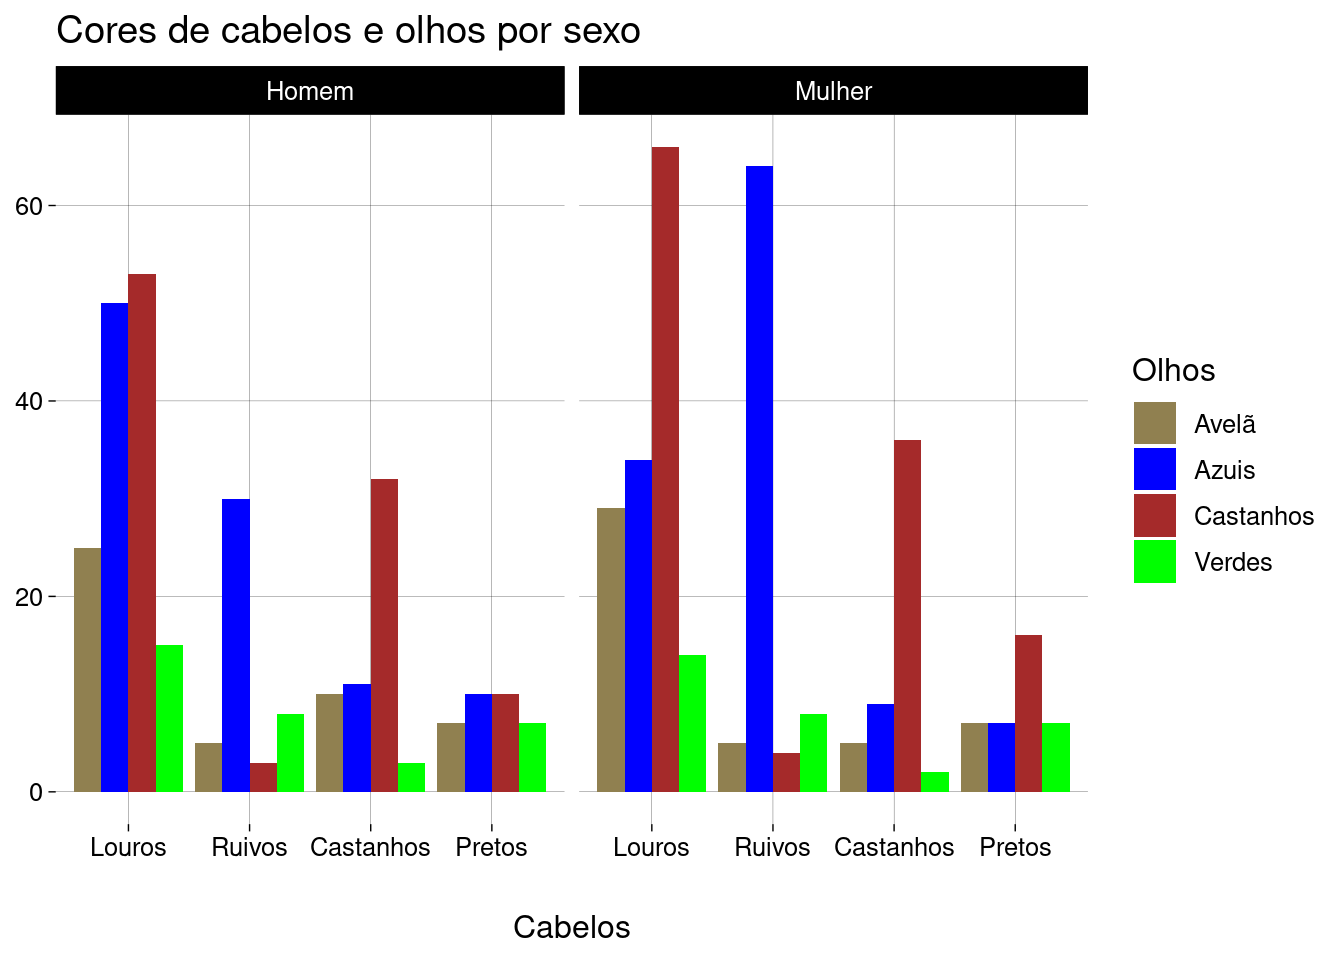
\includegraphics[width=1\linewidth]{_main_files/figure-latex/unnamed-chunk-62-1} \end{center}
\item
  A {\hl{caixa}} vai do valor do {\hl{primeiro quartil}} (embaixo) até o {\hl{terceiro quartil}} (em cima).
\item
  A {\hl{linha horizontal dentro da caixa}} representa o valor da {\hl{mediana}}.
\item
  As {\hl{linhas verticais}} acima e abaixo da caixa (pitorescamente chamadas de ``bigodes'') vão até o {\hl{limite inferior}} (primeiro quartil ${}- 1{,}5 \times \text{IQR}$) e até o {\hl{limite superior}} (terceiro quartil ${}+ 1{,}5 \times \text{IQR}$).
\item
  Neste \emph{boxplot}, não há \emph{outliers}.
\item
  Podemos usar a posição $x$ para desenhar vários \emph{boxplots}, um para cada dieta:

\begin{Shaded}
\begin{Highlighting}[]
\NormalTok{sono }\SpecialCharTok{\%\textgreater{}\%} 
  \FunctionTok{ggplot}\NormalTok{(}\FunctionTok{aes}\NormalTok{(}\AttributeTok{x =}\NormalTok{ vore, }\AttributeTok{y =}\NormalTok{ sleep\_total)) }\SpecialCharTok{+}
    \FunctionTok{geom\_boxplot}\NormalTok{(}\AttributeTok{fill =} \StringTok{\textquotesingle{}gray\textquotesingle{}}\NormalTok{) }\SpecialCharTok{+}
    \FunctionTok{scale\_y\_continuous}\NormalTok{(}\AttributeTok{breaks =} \FunctionTok{seq}\NormalTok{(}\DecValTok{0}\NormalTok{, }\DecValTok{20}\NormalTok{, }\DecValTok{2}\NormalTok{))}
\end{Highlighting}
\end{Shaded}

  \begin{center}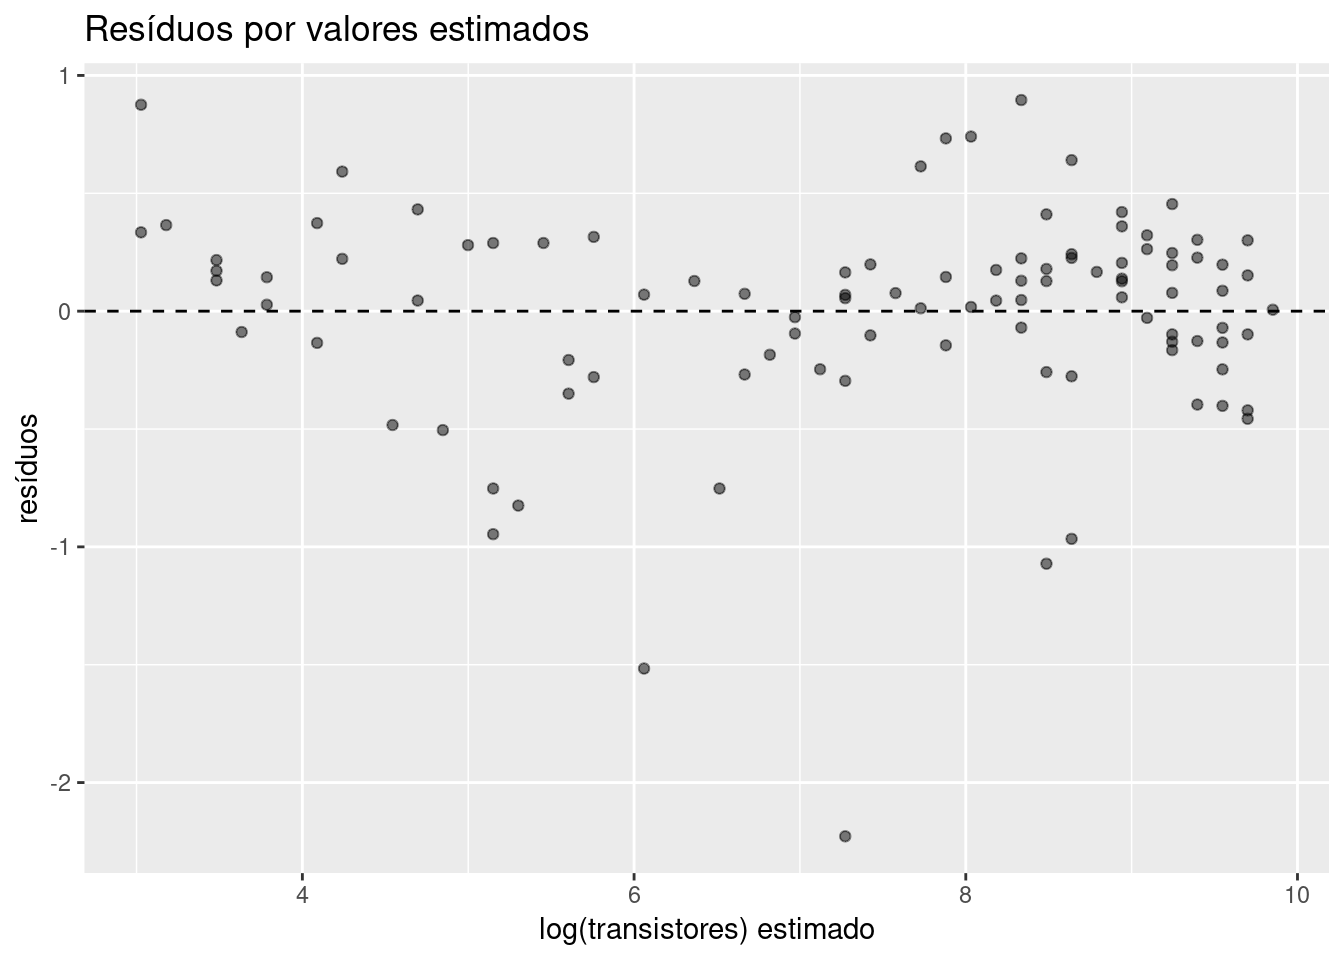
\includegraphics[width=1\linewidth]{_main_files/figure-latex/unnamed-chunk-63-1} \end{center}
\item
  No \emph{boxplot} de onívoros, {\hl{os \emph{outliers} aparecem como pontos isolados,}} acima da caixa, além dos alcances do bigode superior (aliás, onde está bigode superior?).
\item
  \emph{Boxplots} lado a lado são úteis para compararmos grupos diferentes de dados.
\item
  Veja como, com exceção dos insetívoros, as medianas dos grupos são parecidas.
\item
  Veja como carnívoros, insetívoros e herbívoros apresentam maior variação, enquanto onívoros e animais sem dieta registrada apresentam menor variação.
\item
  Vamos combinar, em um só gráfico

  \begin{itemize}
  \item
    Os pontos representando os animais,
  \item
    Os \emph{boxplots},
  \item
    As médias (que podem estar próximas ou distantes das medianas).
  \end{itemize}

\begin{Shaded}
\begin{Highlighting}[]
\NormalTok{sono }\SpecialCharTok{\%\textgreater{}\%} 
  \FunctionTok{ggplot}\NormalTok{(}\FunctionTok{aes}\NormalTok{(}\AttributeTok{x =}\NormalTok{ vore, }\AttributeTok{y =}\NormalTok{ sleep\_total)) }\SpecialCharTok{+}
    \FunctionTok{geom\_boxplot}\NormalTok{(}\AttributeTok{fill =} \StringTok{\textquotesingle{}gray\textquotesingle{}}\NormalTok{) }\SpecialCharTok{+}
    \FunctionTok{scale\_y\_continuous}\NormalTok{(}\AttributeTok{breaks =} \FunctionTok{seq}\NormalTok{(}\DecValTok{0}\NormalTok{, }\DecValTok{20}\NormalTok{, }\DecValTok{2}\NormalTok{)) }\SpecialCharTok{+}
    \FunctionTok{geom\_point}\NormalTok{(}
      \AttributeTok{color =} \StringTok{\textquotesingle{}blue\textquotesingle{}}\NormalTok{, }
      \AttributeTok{alpha =}\NormalTok{ .}\DecValTok{3}
\NormalTok{    ) }\SpecialCharTok{+}
    \FunctionTok{stat\_summary}\NormalTok{(}
      \AttributeTok{fun =}\NormalTok{ mean, }
      \AttributeTok{geom =} \StringTok{\textquotesingle{}point\textquotesingle{}}\NormalTok{, }
      \AttributeTok{color =} \StringTok{\textquotesingle{}red\textquotesingle{}}\NormalTok{, }
      \AttributeTok{shape =} \StringTok{\textquotesingle{}cross\textquotesingle{}}\NormalTok{, }
      \AttributeTok{size =} \DecValTok{5}\NormalTok{,}
      \AttributeTok{stroke =} \DecValTok{1}
\NormalTok{    ) }\SpecialCharTok{+}
    \FunctionTok{labs}\NormalTok{(}
      \AttributeTok{title =} \StringTok{\textquotesingle{}Sono total de diversos mamíferos, por dieta\textquotesingle{}}\NormalTok{,}
      \AttributeTok{subtitle =} \StringTok{\textquotesingle{}(o X vermelho representa a média)\textquotesingle{}}\NormalTok{,}
      \AttributeTok{x =} \StringTok{\textquotesingle{}dieta\textquotesingle{}}\NormalTok{,}
      \AttributeTok{y =} \StringTok{\textquotesingle{}sono total}\SpecialCharTok{\textbackslash{}n}\StringTok{(em horas)\textquotesingle{}}
\NormalTok{    )}
\end{Highlighting}
\end{Shaded}

  \begin{center}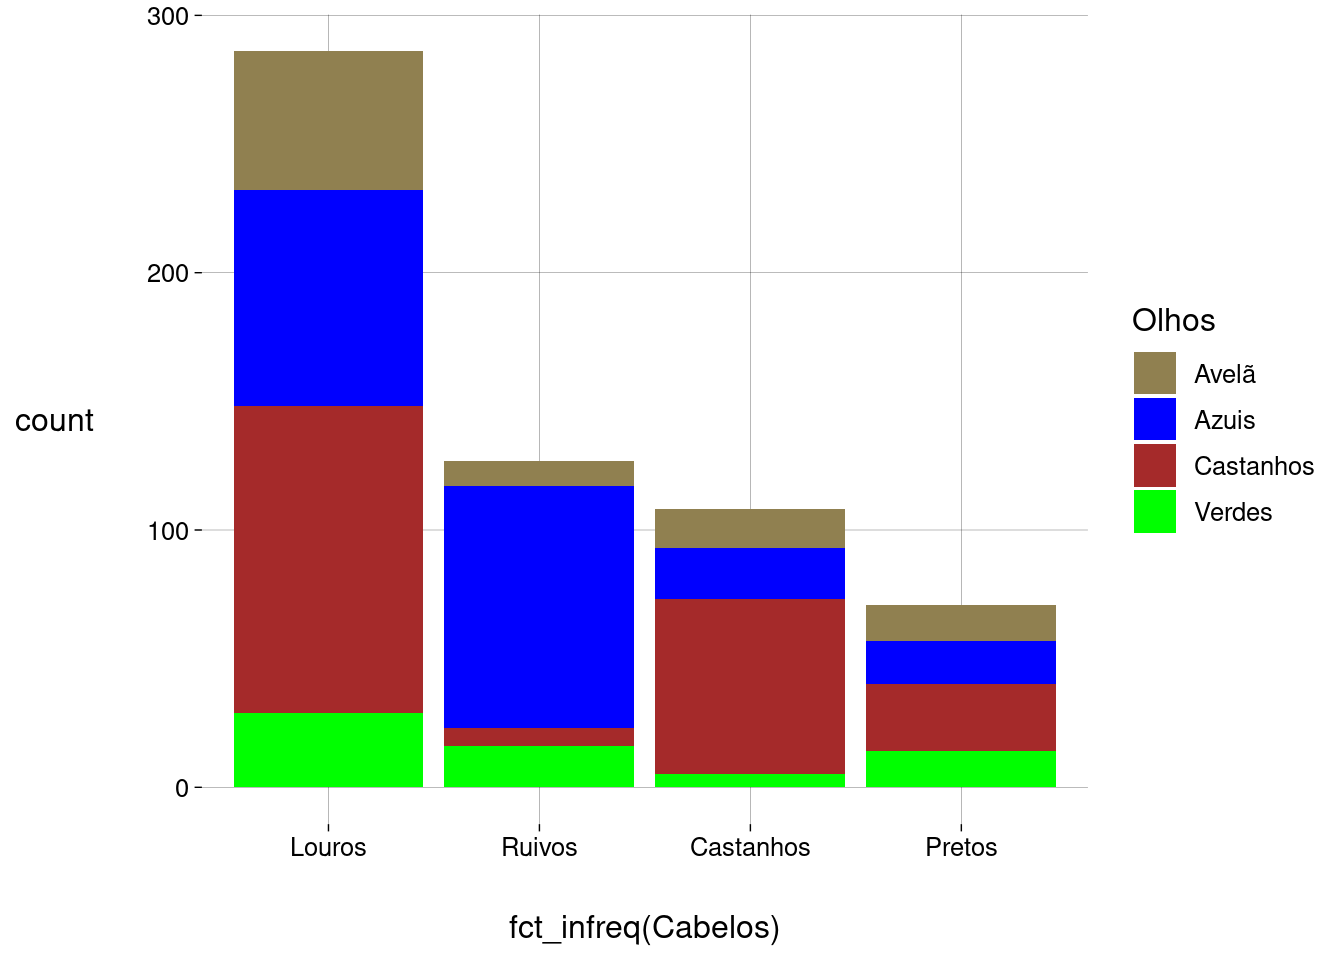
\includegraphics[width=1\linewidth]{_main_files/figure-latex/unnamed-chunk-64-1} \end{center}
\item
  {\hl{Quando a caixa é longa,}} o IQR é grande, e {\hl{os valores estão muito espalhados;}} é o caso dos herbívoros e insetívoros.
\item
  {\hl{Quando a caixa é curta,}} o IQR é pequeno, e {\hl{os valores estão pouco espalhados}}; é o caso dos onívoros. Como o IQR é pequeno, os $4$ mamíferos com mais de $14$ horas de sono são \emph{outliers}.
\item
  Observe, ainda, como os \emph{outliers} ``puxam'' a média dos onívoros para cima.
\end{itemize}

\hypertarget{vuxeddeo-2-3}{%
\section{Vídeo 2}\label{vuxeddeo-2-3}}

\begin{center} \url{https://youtu.be/QqnOvgBXJ-s} \end{center}

\hypertarget{gruxe1ficos-de-barras-e-de-colunas}{%
\section{Gráficos de barras e de colunas}\label{gruxe1ficos-de-barras-e-de-colunas}}

\hypertarget{conjunto-de-dados-2}{%
\subsection{Conjunto de dados}\label{conjunto-de-dados-2}}

\begin{itemize}
\item
  O R tem um \emph{array} de $3$ dimensões com dados sobre as cores dos cabelos e dos olhos de $592$ alunos e alunas de uma universidade americana em $1974$.
\item
  Se pedirmos para o R exibir os dados, veremos {\hl{duas matrizes}}, uma para cada sexo:

\begin{Shaded}
\begin{Highlighting}[]
\NormalTok{HairEyeColor}
\DocumentationTok{\#\# , , Sex = Male}
\DocumentationTok{\#\# }
\DocumentationTok{\#\#        Eye}
\DocumentationTok{\#\# Hair    Brown Blue Hazel Green}
\DocumentationTok{\#\#   Black    32   11    10     3}
\DocumentationTok{\#\#   Brown    53   50    25    15}
\DocumentationTok{\#\#   Red      10   10     7     7}
\DocumentationTok{\#\#   Blond     3   30     5     8}
\DocumentationTok{\#\# }
\DocumentationTok{\#\# , , Sex = Female}
\DocumentationTok{\#\# }
\DocumentationTok{\#\#        Eye}
\DocumentationTok{\#\# Hair    Brown Blue Hazel Green}
\DocumentationTok{\#\#   Black    36    9     5     2}
\DocumentationTok{\#\#   Brown    66   34    29    14}
\DocumentationTok{\#\#   Red      16    7     7     7}
\DocumentationTok{\#\#   Blond     4   64     5     8}
\end{Highlighting}
\end{Shaded}
\item
  Vamos transformar este \emph{array} em um \emph{data frame}.
\item
  O \emph{array} contém apenas os totais de cada classe. Vamos usar a função \texttt{uncount} para gerar uma linha para cada aluno:

\begin{Shaded}
\begin{Highlighting}[]
\NormalTok{df\_orig }\OtherTok{\textless{}{-}} \FunctionTok{as.data.frame}\NormalTok{(HairEyeColor) }\SpecialCharTok{\%\textgreater{}\%} 
  \FunctionTok{uncount}\NormalTok{(Freq) }\SpecialCharTok{\%\textgreater{}\%} 
  \FunctionTok{as\_tibble}\NormalTok{()}

\NormalTok{df\_orig}
\DocumentationTok{\#\# \# A tibble: 592 x 3}
\DocumentationTok{\#\#   Hair  Eye   Sex  }
\DocumentationTok{\#\#   \textless{}fct\textgreater{} \textless{}fct\textgreater{} \textless{}fct\textgreater{}}
\DocumentationTok{\#\# 1 Black Brown Male }
\DocumentationTok{\#\# 2 Black Brown Male }
\DocumentationTok{\#\# 3 Black Brown Male }
\DocumentationTok{\#\# 4 Black Brown Male }
\DocumentationTok{\#\# 5 Black Brown Male }
\DocumentationTok{\#\# 6 Black Brown Male }
\DocumentationTok{\#\# \# ... with 586 more rows}
\end{Highlighting}
\end{Shaded}
\item
  O \texttt{ggplot2} e os outros pacotes do \texttt{tidyverse} foram projetados para trabalhar com \emph{data frames} neste formato, {\hl{com uma observação (um indivíduo, um elemento) por linha.}} É o chamado {\hl{formato \emph{tidy}.}}
\item
  Usando vetores com elementos nomeados, podemos traduzir o conteúdo do \emph{data frame} para português:

\begin{Shaded}
\begin{Highlighting}[]
\NormalTok{cabelo }\OtherTok{\textless{}{-}} \FunctionTok{c}\NormalTok{(}
  \StringTok{\textquotesingle{}Brown\textquotesingle{}} \OtherTok{=} \StringTok{\textquotesingle{}castanhos\textquotesingle{}}\NormalTok{,}
  \StringTok{\textquotesingle{}Blond\textquotesingle{}} \OtherTok{=} \StringTok{\textquotesingle{}louros\textquotesingle{}}\NormalTok{,}
  \StringTok{\textquotesingle{}Black\textquotesingle{}} \OtherTok{=} \StringTok{\textquotesingle{}pretos\textquotesingle{}}\NormalTok{,}
  \StringTok{\textquotesingle{}Red\textquotesingle{}} \OtherTok{=} \StringTok{\textquotesingle{}ruivos\textquotesingle{}}
\NormalTok{)}

\NormalTok{olhos }\OtherTok{\textless{}{-}} \FunctionTok{c}\NormalTok{(}
  \StringTok{\textquotesingle{}Brown\textquotesingle{}} \OtherTok{=} \StringTok{\textquotesingle{}castanhos\textquotesingle{}}\NormalTok{,}
  \StringTok{\textquotesingle{}Blue\textquotesingle{}} \OtherTok{=} \StringTok{\textquotesingle{}azuis\textquotesingle{}}\NormalTok{,}
  \StringTok{\textquotesingle{}Hazel\textquotesingle{}} \OtherTok{=} \StringTok{\textquotesingle{}avelã\textquotesingle{}}\NormalTok{,}
  \StringTok{\textquotesingle{}Green\textquotesingle{}} \OtherTok{=} \StringTok{\textquotesingle{}verdes\textquotesingle{}}
\NormalTok{)}

\NormalTok{sexo }\OtherTok{\textless{}{-}} \FunctionTok{c}\NormalTok{(}
  \StringTok{\textquotesingle{}Male\textquotesingle{}} \OtherTok{=} \StringTok{\textquotesingle{}homem\textquotesingle{}}\NormalTok{,}
  \StringTok{\textquotesingle{}Female\textquotesingle{}} \OtherTok{=} \StringTok{\textquotesingle{}mulher\textquotesingle{}}
\NormalTok{)}

\NormalTok{df }\OtherTok{\textless{}{-}}\NormalTok{ df\_orig }\SpecialCharTok{\%\textgreater{}\%} 
  \FunctionTok{transmute}\NormalTok{(}
    \AttributeTok{cabelos =}\NormalTok{ cabelo[Hair],}
    \AttributeTok{olhos =}\NormalTok{ olhos[Eye],}
    \AttributeTok{sexo =}\NormalTok{ sexo[Sex]}
\NormalTok{  )}
\end{Highlighting}
\end{Shaded}
\item
  Um sumário:

\begin{Shaded}
\begin{Highlighting}[]
\NormalTok{df }\SpecialCharTok{\%\textgreater{}\%} \FunctionTok{dfSummary}\NormalTok{() }\SpecialCharTok{\%\textgreater{}\%} \FunctionTok{print}\NormalTok{()}
\end{Highlighting}
\end{Shaded}

  \begin{longtable}[]{@{}
    >{\raggedright\arraybackslash}p{(\columnwidth - 6\tabcolsep) * \real{0.1918}}
    >{\raggedright\arraybackslash}p{(\columnwidth - 6\tabcolsep) * \real{0.3425}}
    >{\raggedright\arraybackslash}p{(\columnwidth - 6\tabcolsep) * \real{0.3151}}
    >{\raggedright\arraybackslash}p{(\columnwidth - 6\tabcolsep) * \real{0.1507}}@{}}
  \toprule
  \begin{minipage}[b]{\linewidth}\raggedright
  Variável
  \end{minipage} & \begin{minipage}[b]{\linewidth}\raggedright
  Estatísticas / Valores
  \end{minipage} & \begin{minipage}[b]{\linewidth}\raggedright
  Freqs (\% de Válidos)
  \end{minipage} & \begin{minipage}[b]{\linewidth}\raggedright
  Faltante
  \end{minipage} \\
  \midrule
  \endhead
  \begin{minipage}[t]{\linewidth}\raggedright
  cabelos\\
  {[}character{]}\strut
  \end{minipage} & \begin{minipage}[t]{\linewidth}\raggedright
  1. castanhos\\
  2. louros\\
  3. pretos\\
  4. ruivos\strut
  \end{minipage} & \begin{minipage}[t]{\linewidth}\raggedright
  108 (18,2\%)\\
  286 (48,3\%)\\
  71 (12,0\%)\\
  127 (21,5\%)\strut
  \end{minipage} & \begin{minipage}[t]{\linewidth}\raggedright
  0\\
  (0,0\%)\strut
  \end{minipage} \\
  \begin{minipage}[t]{\linewidth}\raggedright
  olhos\\
  {[}character{]}\strut
  \end{minipage} & \begin{minipage}[t]{\linewidth}\raggedright
  1. avelã\\
  2. azuis\\
  3. castanhos\\
  4. verdes\strut
  \end{minipage} & \begin{minipage}[t]{\linewidth}\raggedright
  93 (15,7\%)\\
  215 (36,3\%)\\
  220 (37,2\%)\\
  64 (10,8\%)\strut
  \end{minipage} & \begin{minipage}[t]{\linewidth}\raggedright
  0\\
  (0,0\%)\strut
  \end{minipage} \\
  \begin{minipage}[t]{\linewidth}\raggedright
  sexo\\
  {[}character{]}\strut
  \end{minipage} & \begin{minipage}[t]{\linewidth}\raggedright
  1. homem\\
  2. mulher\strut
  \end{minipage} & \begin{minipage}[t]{\linewidth}\raggedright
  279 (47,1\%)\\
  313 (52,9\%)\strut
  \end{minipage} & \begin{minipage}[t]{\linewidth}\raggedright
  0\\
  (0,0\%)\strut
  \end{minipage} \\
  \bottomrule
  \end{longtable}
\end{itemize}

\hypertarget{gerando-gruxe1ficos-de-barras}{%
\subsection{Gerando gráficos de barras}\label{gerando-gruxe1ficos-de-barras}}

\begin{itemize}
\item
  Um {\hl{gráfico de barras}} contém uma barra para cada valor de uma {\hl{variável categórica.}}
\item
  {\hl{Usamos \texttt{geom\_bar} para gerar um gráfico de barras}} de cores de cabelo:

\begin{Shaded}
\begin{Highlighting}[]
\NormalTok{df }\SpecialCharTok{\%\textgreater{}\%} 
  \FunctionTok{ggplot}\NormalTok{(}\FunctionTok{aes}\NormalTok{(}\AttributeTok{x =}\NormalTok{ cabelos)) }\SpecialCharTok{+}
    \FunctionTok{geom\_bar}\NormalTok{() }\SpecialCharTok{+}
    \FunctionTok{labs}\NormalTok{(}\AttributeTok{y =} \ConstantTok{NULL}\NormalTok{)}
\end{Highlighting}
\end{Shaded}

  \begin{center}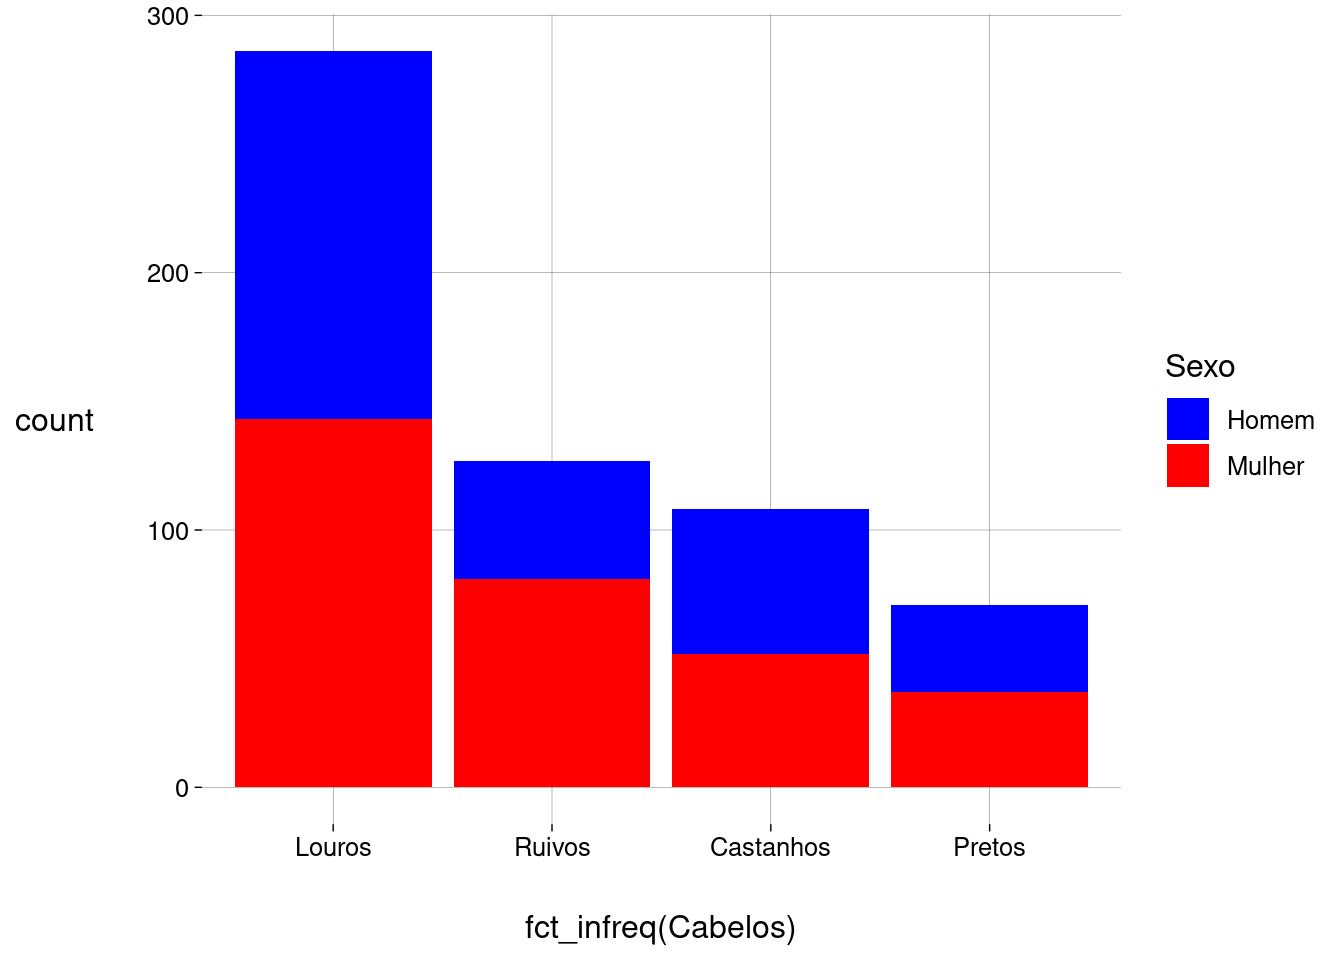
\includegraphics[width=1\linewidth]{_main_files/figure-latex/unnamed-chunk-70-1} \end{center}

  \begin{rmdimportant}

  \textbf{Gráfico de barras $\times$ histograma:}

  \begin{itemize}
  \item
    {\hl{Os dois tipos de gráficos mostram a frequência}} (quantidade de elementos) {\hl{no eixo vertical}}.
  \item
    No {\hl{gráfico de barras}}:

    \begin{itemize}
    \item
      A variável é {\hl{categórica}} (nominal).
    \item
      {\hl{Cada barra}} corresponde a {\hl{um valor}} da variável.
    \item
      {\hl{As barras não se tocam}}, enfatizando o fato de que a variável é categórica.
    \end{itemize}
  \item
    No {\hl{histograma}} (\protect\hyperlink{histograma1}{veja o exemplo}):

    \begin{itemize}
    \item
      A variável é {\hl{quantitativa}} (intervalar ou racional).
    \item
      {\hl{Cada barra}} corresponde a {\hl{uma classe de valores}} da variável.
    \item
      {\hl{As barras se tocam}}, para enfatizar que as classes são contíguas.
    \end{itemize}
  \end{itemize}

  \end{rmdimportant}
\item
  Um gráfico de barras é mais legível quando as barras são mostradas em ordem crescente ou decrescente.
\item
  Embora os valores da variável \texttt{cabelos} sejam \emph{strings}, podemos aplicar a eles funções que manipulam fatores.
\item
  A {\hl{função \texttt{fct\_infreq}}}, do pacote \texttt{forcats}, ordena os valores em {\hl{ordem decrescente de frequência}}.
\item
  A {\hl{função \texttt{fct\_rev}}}, também do pacote \texttt{forcats}, {\hl{inverte a ordenação.}}

\begin{Shaded}
\begin{Highlighting}[]
\NormalTok{df }\SpecialCharTok{\%\textgreater{}\%} 
  \FunctionTok{ggplot}\NormalTok{(}\FunctionTok{aes}\NormalTok{(}\AttributeTok{x =} \FunctionTok{fct\_rev}\NormalTok{(}\FunctionTok{fct\_infreq}\NormalTok{(cabelos)))) }\SpecialCharTok{+}
    \FunctionTok{geom\_bar}\NormalTok{() }\SpecialCharTok{+}
    \FunctionTok{labs}\NormalTok{(}
      \AttributeTok{x =} \StringTok{\textquotesingle{}cabelos\textquotesingle{}}\NormalTok{,}
      \AttributeTok{y =} \ConstantTok{NULL}
\NormalTok{    )}
\end{Highlighting}
\end{Shaded}

  \begin{center}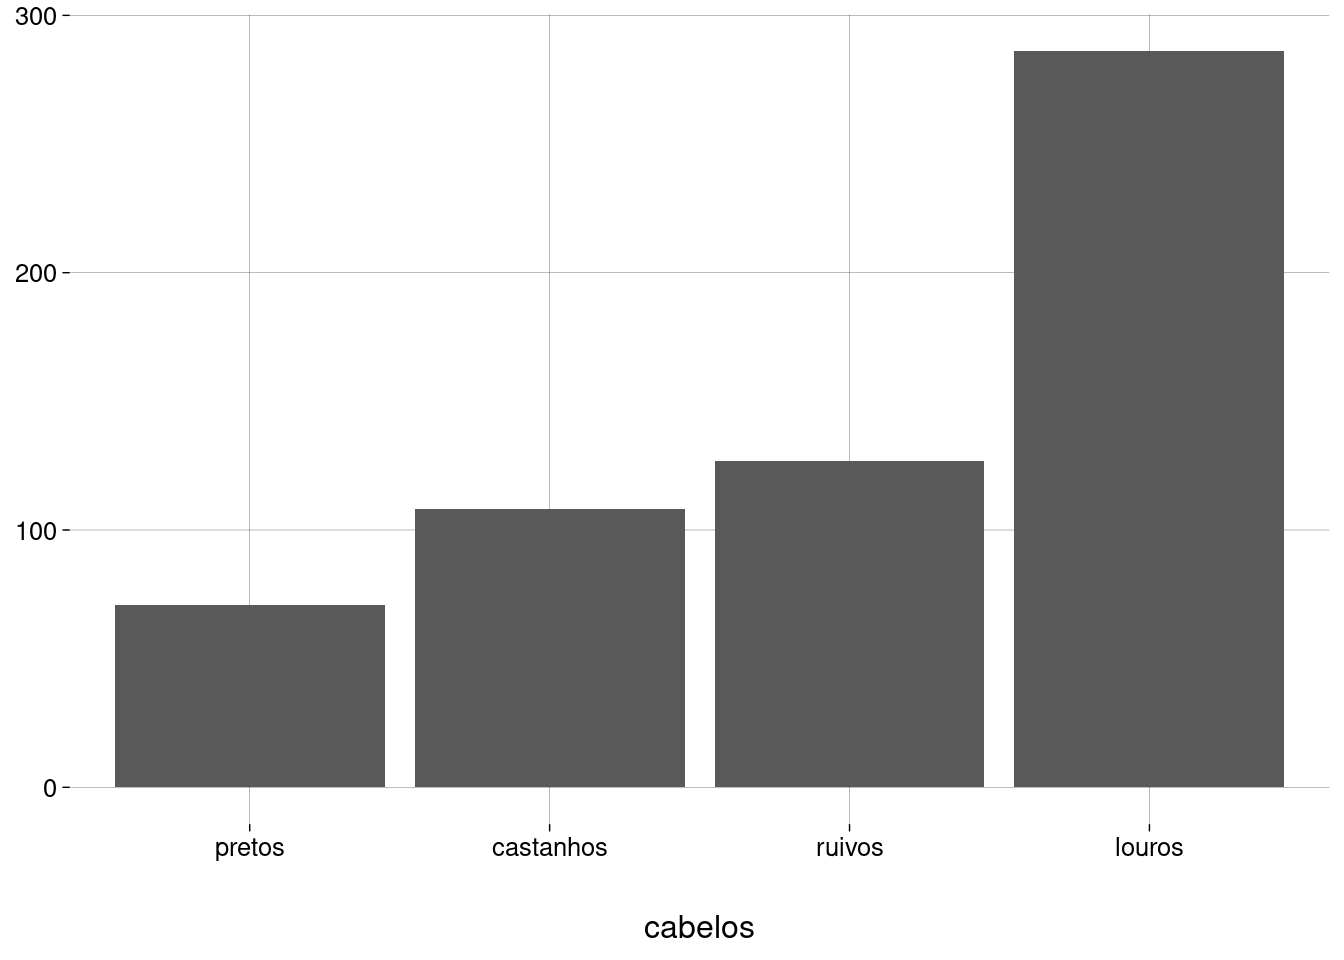
\includegraphics[width=1\linewidth]{_main_files/figure-latex/unnamed-chunk-71-1} \end{center}
\item
  A posição $x$ e a altura de cada barra são estéticas: {\hl{a posição $x$ representa a cor dos cabelos}}, e {\hl{a altura representa a frequência daquela cor}}.
\item
  Vamos acrescentar mais uma estética: {\hl{a cor de preenchimento vai representar o sexo}}.

\begin{Shaded}
\begin{Highlighting}[]
\NormalTok{df }\SpecialCharTok{\%\textgreater{}\%} 
  \FunctionTok{ggplot}\NormalTok{(}\FunctionTok{aes}\NormalTok{(}\AttributeTok{x =} \FunctionTok{fct\_rev}\NormalTok{(}\FunctionTok{fct\_infreq}\NormalTok{(cabelos)), }\AttributeTok{fill =}\NormalTok{ sexo)) }\SpecialCharTok{+}
    \FunctionTok{geom\_bar}\NormalTok{() }\SpecialCharTok{+}
    \FunctionTok{labs}\NormalTok{(}
      \AttributeTok{x =} \StringTok{\textquotesingle{}cabelos\textquotesingle{}}\NormalTok{,}
      \AttributeTok{y =} \ConstantTok{NULL}
\NormalTok{    )}
\end{Highlighting}
\end{Shaded}

  \begin{center}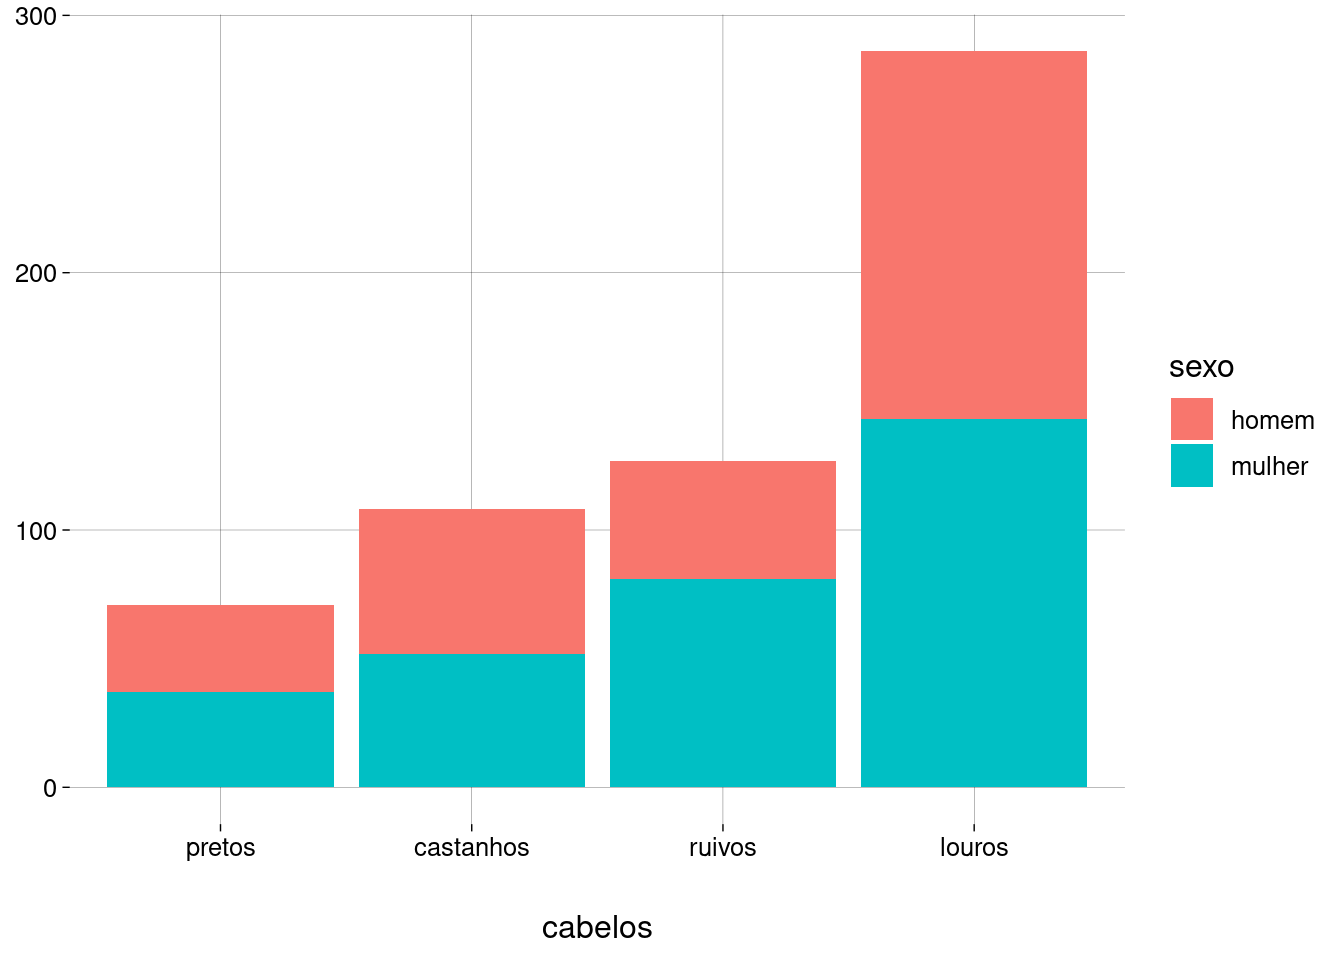
\includegraphics[width=1\linewidth]{_main_files/figure-latex/unnamed-chunk-72-1} \end{center}
\item
  Se a cor dos homens incomoda você, altere a escala que especifica o preenchimento (\texttt{scale\_fill\_discrete}):

\begin{Shaded}
\begin{Highlighting}[]
\NormalTok{df }\SpecialCharTok{\%\textgreater{}\%} 
  \FunctionTok{ggplot}\NormalTok{(}\FunctionTok{aes}\NormalTok{(}\AttributeTok{x =} \FunctionTok{fct\_rev}\NormalTok{(}\FunctionTok{fct\_infreq}\NormalTok{(cabelos)), }\AttributeTok{fill =}\NormalTok{ sexo)) }\SpecialCharTok{+}
    \FunctionTok{geom\_bar}\NormalTok{() }\SpecialCharTok{+}
    \FunctionTok{scale\_fill\_discrete}\NormalTok{(}\AttributeTok{type =} \FunctionTok{c}\NormalTok{(}\StringTok{\textquotesingle{}blue\textquotesingle{}}\NormalTok{, }\StringTok{\textquotesingle{}red\textquotesingle{}}\NormalTok{)) }\SpecialCharTok{+}
    \FunctionTok{labs}\NormalTok{(}
      \AttributeTok{x =} \StringTok{\textquotesingle{}cabelos\textquotesingle{}}\NormalTok{,}
      \AttributeTok{y =} \ConstantTok{NULL}
\NormalTok{    )}
\end{Highlighting}
\end{Shaded}

  \begin{center}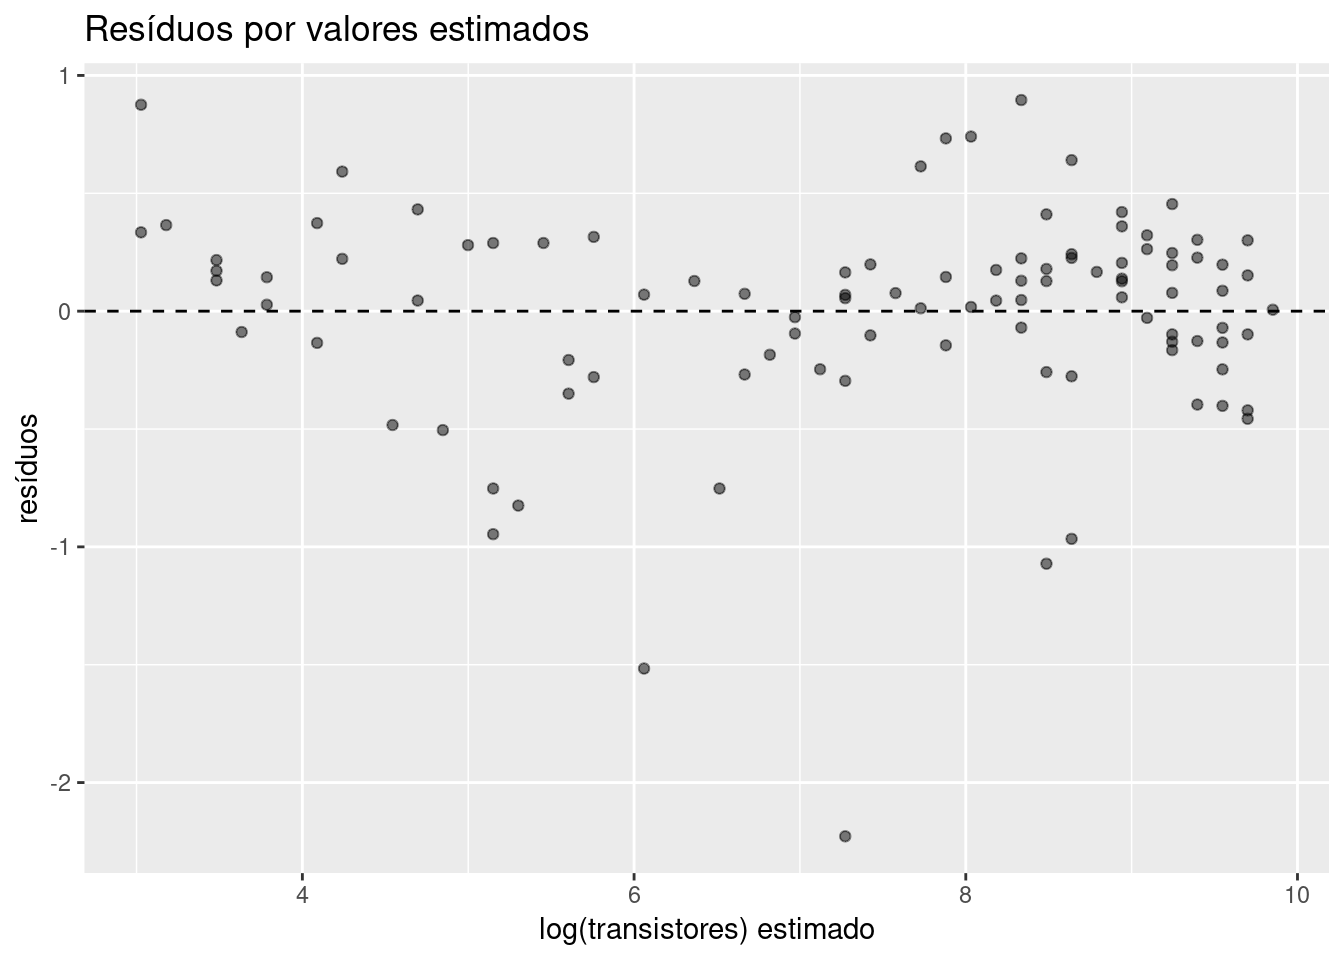
\includegraphics[width=1\linewidth]{_main_files/figure-latex/unnamed-chunk-73-1} \end{center}
\item
  {\hl{Podemos fazer um gráfico de barras horizontais com \texttt{coord\_flip}.}} Isto geralmente é útil quando os rótulos das barras são longos:

\begin{Shaded}
\begin{Highlighting}[]
\NormalTok{df }\SpecialCharTok{\%\textgreater{}\%} 
  \FunctionTok{ggplot}\NormalTok{(}\FunctionTok{aes}\NormalTok{(}\AttributeTok{x =} \FunctionTok{fct\_rev}\NormalTok{(}\FunctionTok{fct\_infreq}\NormalTok{(cabelos)), }\AttributeTok{fill =}\NormalTok{ sexo)) }\SpecialCharTok{+}
    \FunctionTok{geom\_bar}\NormalTok{() }\SpecialCharTok{+}
    \FunctionTok{scale\_fill\_discrete}\NormalTok{(}\AttributeTok{type =} \FunctionTok{c}\NormalTok{(}\StringTok{\textquotesingle{}blue\textquotesingle{}}\NormalTok{, }\StringTok{\textquotesingle{}red\textquotesingle{}}\NormalTok{)) }\SpecialCharTok{+}
    \FunctionTok{labs}\NormalTok{(}
      \AttributeTok{x =} \StringTok{\textquotesingle{}cabelos\textquotesingle{}}\NormalTok{,}
      \AttributeTok{y =} \ConstantTok{NULL}
\NormalTok{    ) }\SpecialCharTok{+}
    \FunctionTok{coord\_flip}\NormalTok{()}
\end{Highlighting}
\end{Shaded}

  \begin{center}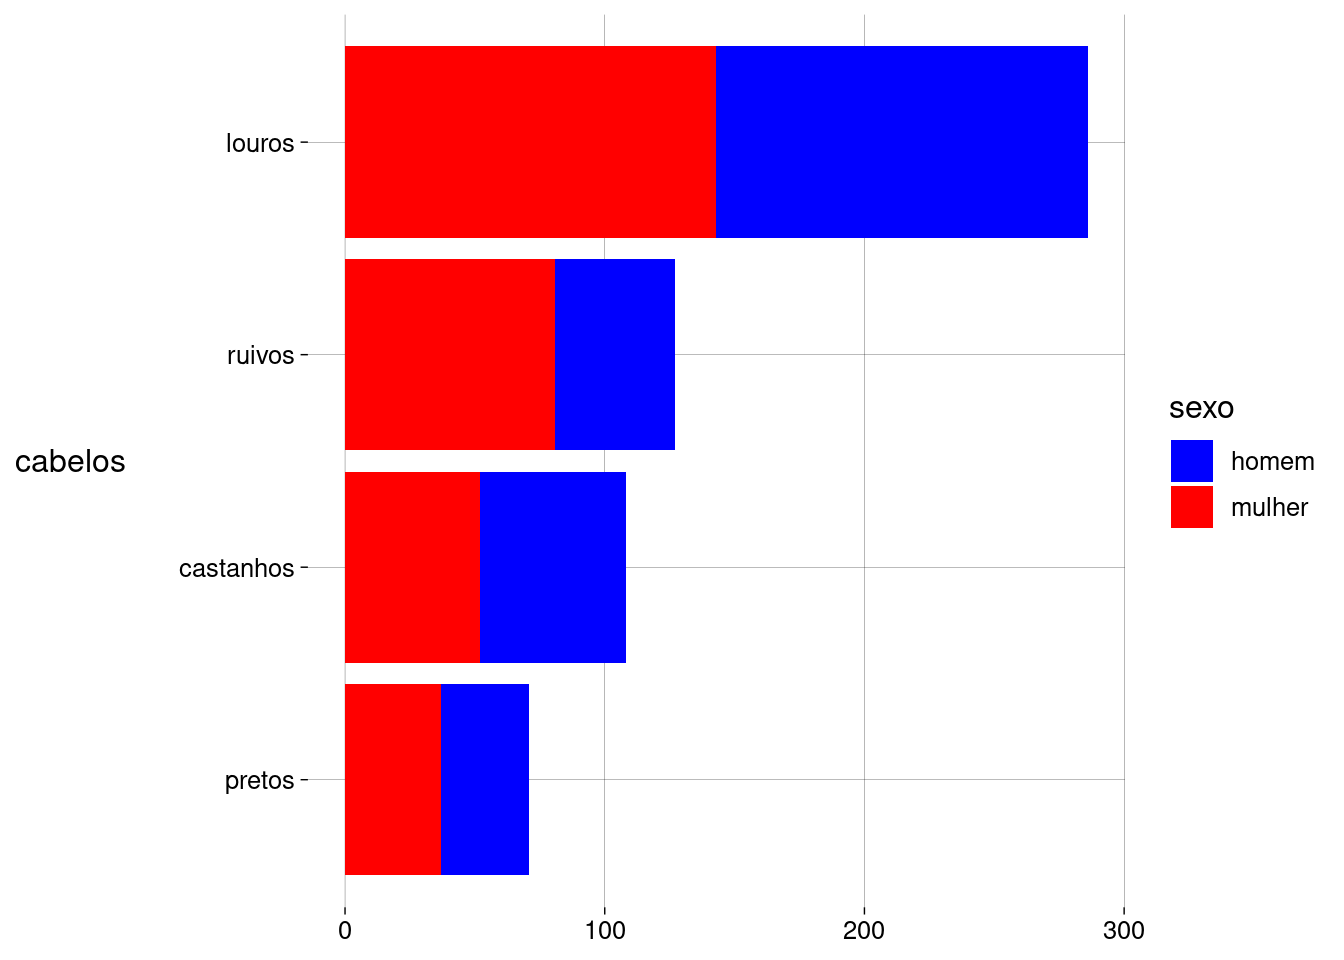
\includegraphics[width=1\linewidth]{_main_files/figure-latex/unnamed-chunk-74-1} \end{center}
\item
  Você consegue dizer se há mais homens ou mulheres com cabelos pretos? E castanhos? E ruivos?
\item
  Se posicionarmos as barras lado a lado, fica mais fácil responder.
\item
  Usamos o argumento \texttt{position\ =\ \textquotesingle{}dodge\textquotesingle{}} de \texttt{geom\_bar}. ``\emph{Dodge}'' significa ``esquivar-se'', em inglês.

\begin{Shaded}
\begin{Highlighting}[]
\NormalTok{df }\SpecialCharTok{\%\textgreater{}\%} 
  \FunctionTok{ggplot}\NormalTok{(}\FunctionTok{aes}\NormalTok{(}\AttributeTok{x =} \FunctionTok{fct\_rev}\NormalTok{(}\FunctionTok{fct\_infreq}\NormalTok{(cabelos)), }\AttributeTok{fill =}\NormalTok{ sexo)) }\SpecialCharTok{+}
    \FunctionTok{geom\_bar}\NormalTok{(}\AttributeTok{position =} \StringTok{\textquotesingle{}dodge\textquotesingle{}}\NormalTok{) }\SpecialCharTok{+}
    \FunctionTok{labs}\NormalTok{(}
      \AttributeTok{x =} \StringTok{\textquotesingle{}cabelos\textquotesingle{}}\NormalTok{,}
      \AttributeTok{y =} \ConstantTok{NULL}
\NormalTok{    ) }\SpecialCharTok{+}
    \FunctionTok{scale\_fill\_discrete}\NormalTok{(}\AttributeTok{type =} \FunctionTok{c}\NormalTok{(}\StringTok{\textquotesingle{}blue\textquotesingle{}}\NormalTok{, }\StringTok{\textquotesingle{}red\textquotesingle{}}\NormalTok{))}
\end{Highlighting}
\end{Shaded}

  \begin{center}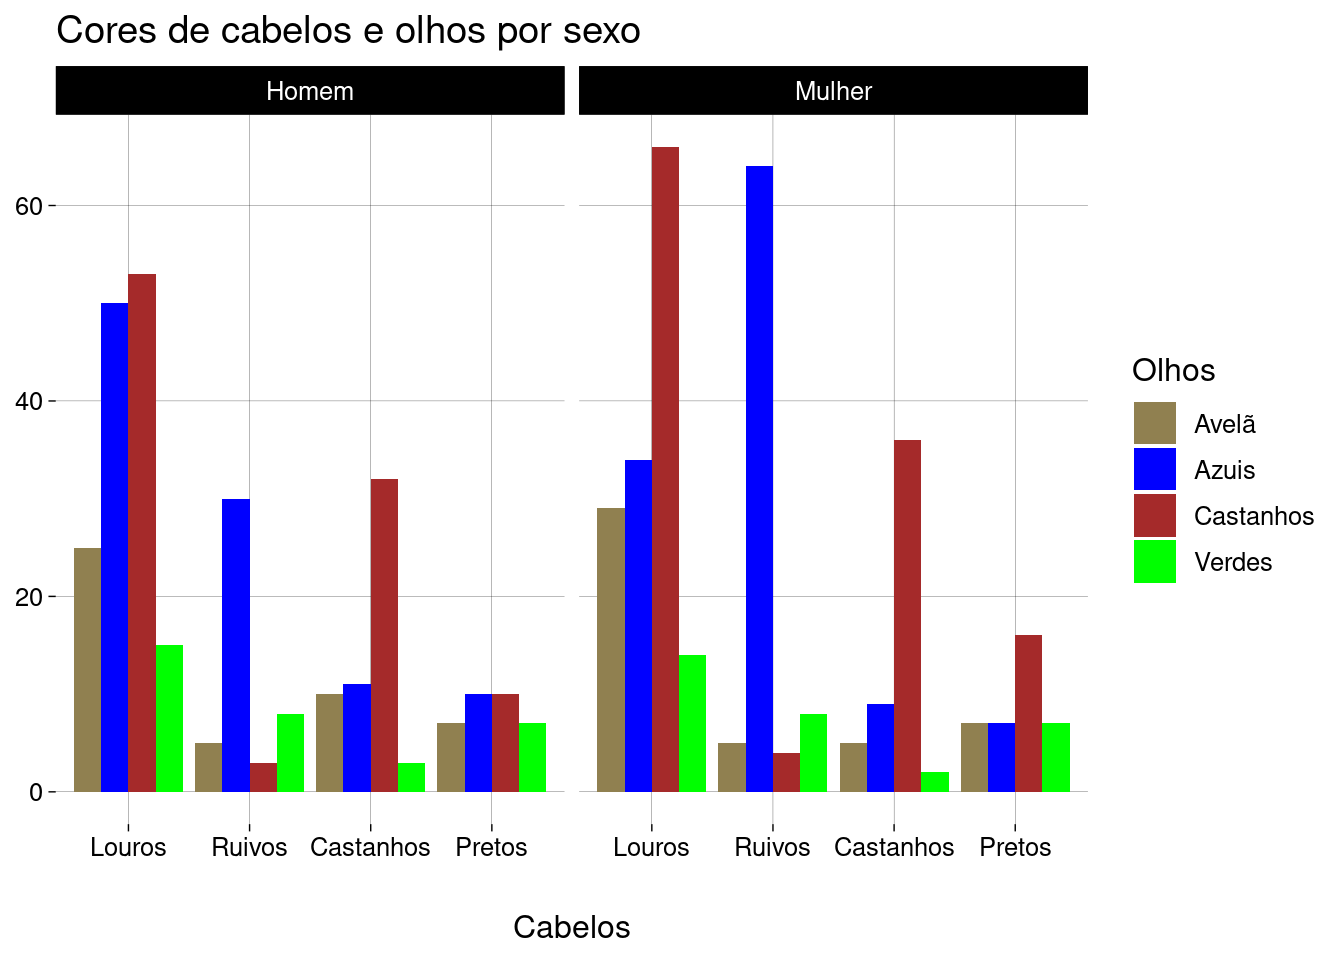
\includegraphics[width=1\linewidth]{_main_files/figure-latex/unnamed-chunk-75-1} \end{center}
\item
  Agora vamos examinar a relação entre as cores dos olhos e as cores dos cabelos:

\begin{Shaded}
\begin{Highlighting}[]
\NormalTok{df }\SpecialCharTok{\%\textgreater{}\%} 
  \FunctionTok{ggplot}\NormalTok{(}\FunctionTok{aes}\NormalTok{(}\AttributeTok{x =} \FunctionTok{fct\_rev}\NormalTok{(}\FunctionTok{fct\_infreq}\NormalTok{(cabelos)), }\AttributeTok{fill =}\NormalTok{ olhos)) }\SpecialCharTok{+}
    \FunctionTok{geom\_bar}\NormalTok{() }\SpecialCharTok{+}
    \FunctionTok{scale\_fill\_discrete}\NormalTok{(}
      \AttributeTok{type =} \FunctionTok{c}\NormalTok{(}\StringTok{\textquotesingle{}\#908050\textquotesingle{}}\NormalTok{, }\StringTok{\textquotesingle{}blue\textquotesingle{}}\NormalTok{, }\StringTok{\textquotesingle{}brown\textquotesingle{}}\NormalTok{, }\StringTok{\textquotesingle{}green\textquotesingle{}}\NormalTok{)}
\NormalTok{    ) }\SpecialCharTok{+}
    \FunctionTok{labs}\NormalTok{(}
      \AttributeTok{x =} \StringTok{\textquotesingle{}cabelos\textquotesingle{}}\NormalTok{,}
      \AttributeTok{y =} \ConstantTok{NULL}
\NormalTok{    )}
\end{Highlighting}
\end{Shaded}

  \begin{center}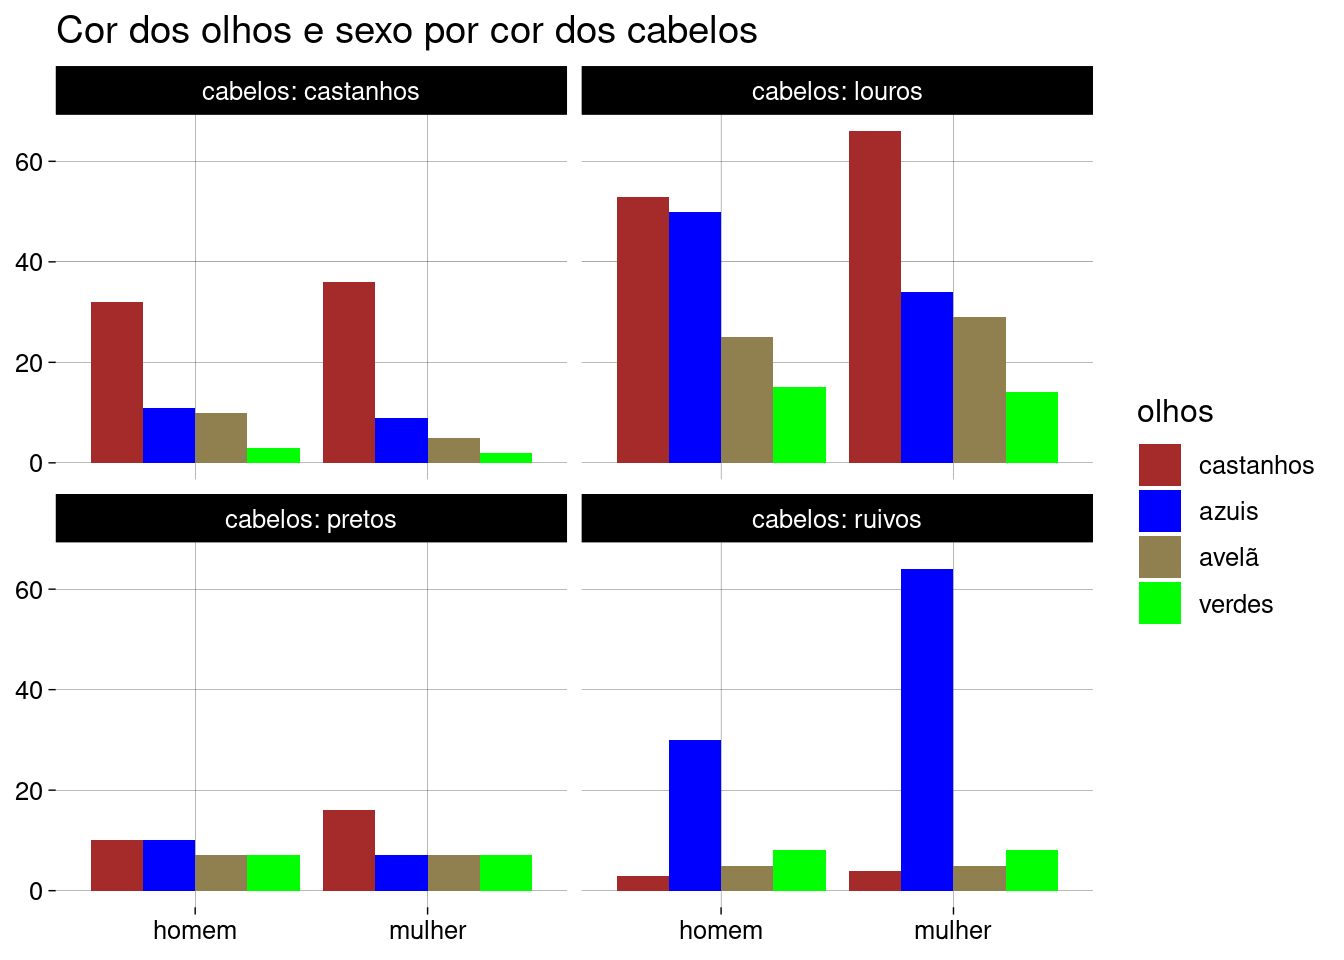
\includegraphics[width=1\linewidth]{_main_files/figure-latex/unnamed-chunk-76-1} \end{center}
\item
  Ou, com barras lado a lado:

\begin{Shaded}
\begin{Highlighting}[]
\NormalTok{df }\SpecialCharTok{\%\textgreater{}\%} 
  \FunctionTok{ggplot}\NormalTok{(}\FunctionTok{aes}\NormalTok{(}\AttributeTok{x =} \FunctionTok{fct\_rev}\NormalTok{(}\FunctionTok{fct\_infreq}\NormalTok{(cabelos)), }\AttributeTok{fill =}\NormalTok{ olhos)) }\SpecialCharTok{+}
    \FunctionTok{geom\_bar}\NormalTok{(}\AttributeTok{position =} \StringTok{\textquotesingle{}dodge\textquotesingle{}}\NormalTok{) }\SpecialCharTok{+}
    \FunctionTok{scale\_fill\_discrete}\NormalTok{(}
      \AttributeTok{type =} \FunctionTok{c}\NormalTok{(}\StringTok{\textquotesingle{}\#908050\textquotesingle{}}\NormalTok{, }\StringTok{\textquotesingle{}blue\textquotesingle{}}\NormalTok{, }\StringTok{\textquotesingle{}brown\textquotesingle{}}\NormalTok{, }\StringTok{\textquotesingle{}green\textquotesingle{}}\NormalTok{)}
\NormalTok{    ) }\SpecialCharTok{+}
    \FunctionTok{labs}\NormalTok{(}
      \AttributeTok{x =} \StringTok{\textquotesingle{}cabelos\textquotesingle{}}\NormalTok{,}
      \AttributeTok{y =} \ConstantTok{NULL}
\NormalTok{    )}
\end{Highlighting}
\end{Shaded}

  \begin{center}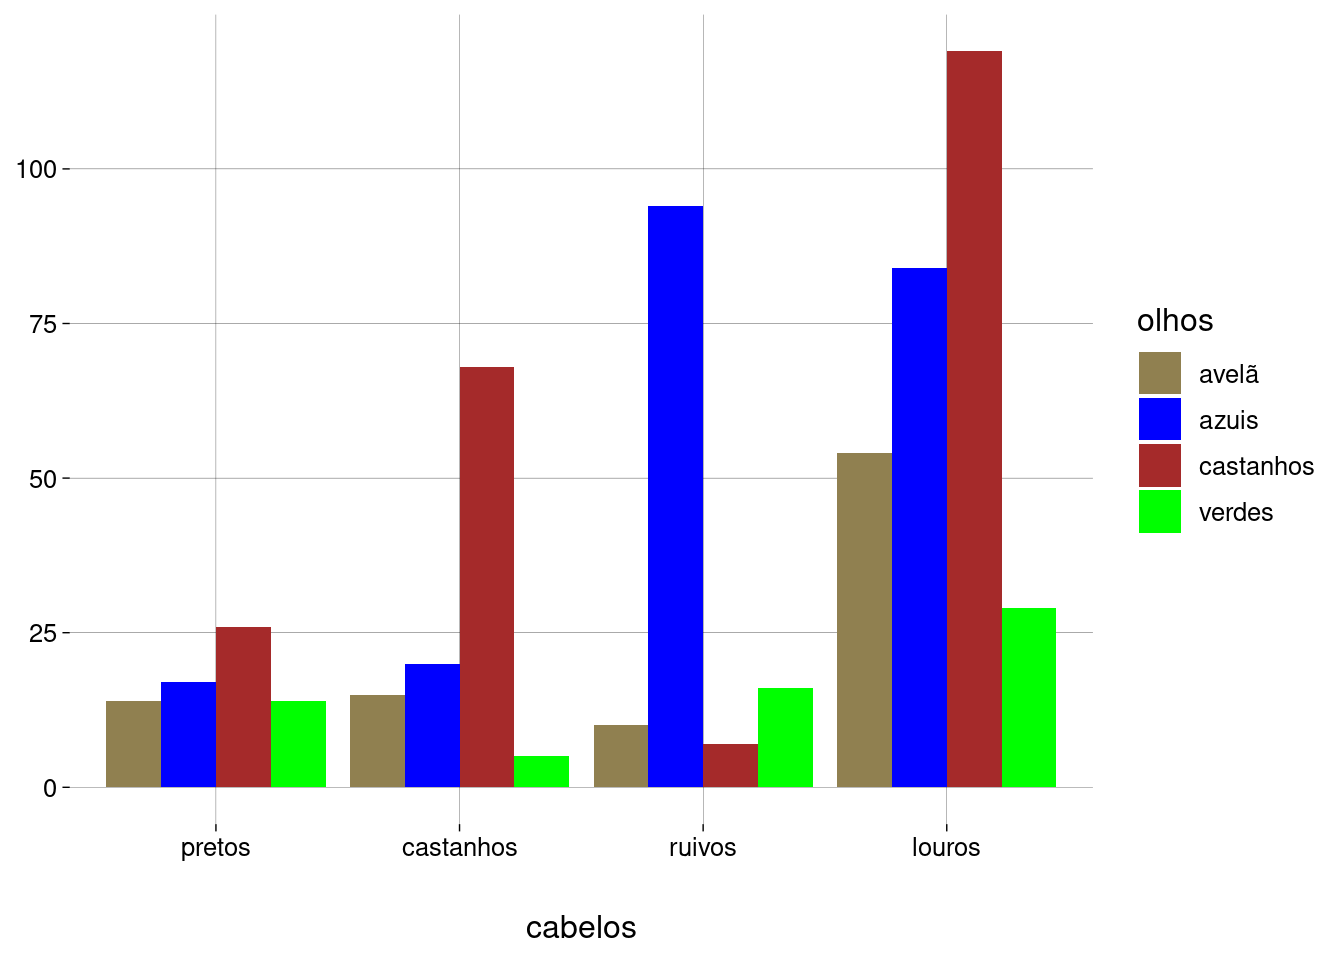
\includegraphics[width=1\linewidth]{_main_files/figure-latex/unnamed-chunk-77-1} \end{center}
\item
  Observações e perguntas:

  \begin{enumerate}
  \def\labelenumi{\arabic{enumi}.}
  \item
    Há mais pessoas louras de olhos castanhos do que louras de olhos azuis. O esperado não seria mais pessoas louras de olhos azuis? Pessoas louras de olhos castanhos pintaram os cabelos?
  \item
    Há muito mais ruivos de olhos azuis do que ruivos de olhos verdes. Não deveria ser o contrário? Também são pessoas que pintaram os cabelos de ruivo? Ou houve erro no registro das cores dos olhos?
  \end{enumerate}
\item
  Para incluir o sexo, podemos {\hl{facetar}} o gráfico. Usando \texttt{facet\_wrap}\footnote{O nome da variável segundo a qual facetar deve aparecer depois de um \texttt{\textasciitilde{}}.}, geramos dois subgráficos lado a lado:

\begin{Shaded}
\begin{Highlighting}[]
\NormalTok{df }\SpecialCharTok{\%\textgreater{}\%} 
  \FunctionTok{ggplot}\NormalTok{(}\FunctionTok{aes}\NormalTok{(}\AttributeTok{x =} \FunctionTok{fct\_rev}\NormalTok{(}\FunctionTok{fct\_infreq}\NormalTok{(cabelos)), }\AttributeTok{fill =}\NormalTok{ olhos)) }\SpecialCharTok{+}
    \FunctionTok{geom\_bar}\NormalTok{(}\AttributeTok{position =} \StringTok{\textquotesingle{}dodge\textquotesingle{}}\NormalTok{) }\SpecialCharTok{+}
    \FunctionTok{scale\_fill\_discrete}\NormalTok{(}\AttributeTok{type =} \FunctionTok{c}\NormalTok{(}\StringTok{\textquotesingle{}\#908050\textquotesingle{}}\NormalTok{, }\StringTok{\textquotesingle{}blue\textquotesingle{}}\NormalTok{, }\StringTok{\textquotesingle{}brown\textquotesingle{}}\NormalTok{, }\StringTok{\textquotesingle{}green\textquotesingle{}}\NormalTok{)) }\SpecialCharTok{+}
    \FunctionTok{facet\_wrap}\NormalTok{(}\SpecialCharTok{\textasciitilde{}}\NormalTok{sexo) }\SpecialCharTok{+}
    \FunctionTok{labs}\NormalTok{(}
      \AttributeTok{title =} \StringTok{\textquotesingle{}Cores de cabelos e olhos por sexo\textquotesingle{}}\NormalTok{,}
      \AttributeTok{y =} \ConstantTok{NULL}\NormalTok{,}
      \AttributeTok{x =} \StringTok{\textquotesingle{}cabelos\textquotesingle{}}
\NormalTok{    )}
\end{Highlighting}
\end{Shaded}

  \begin{center}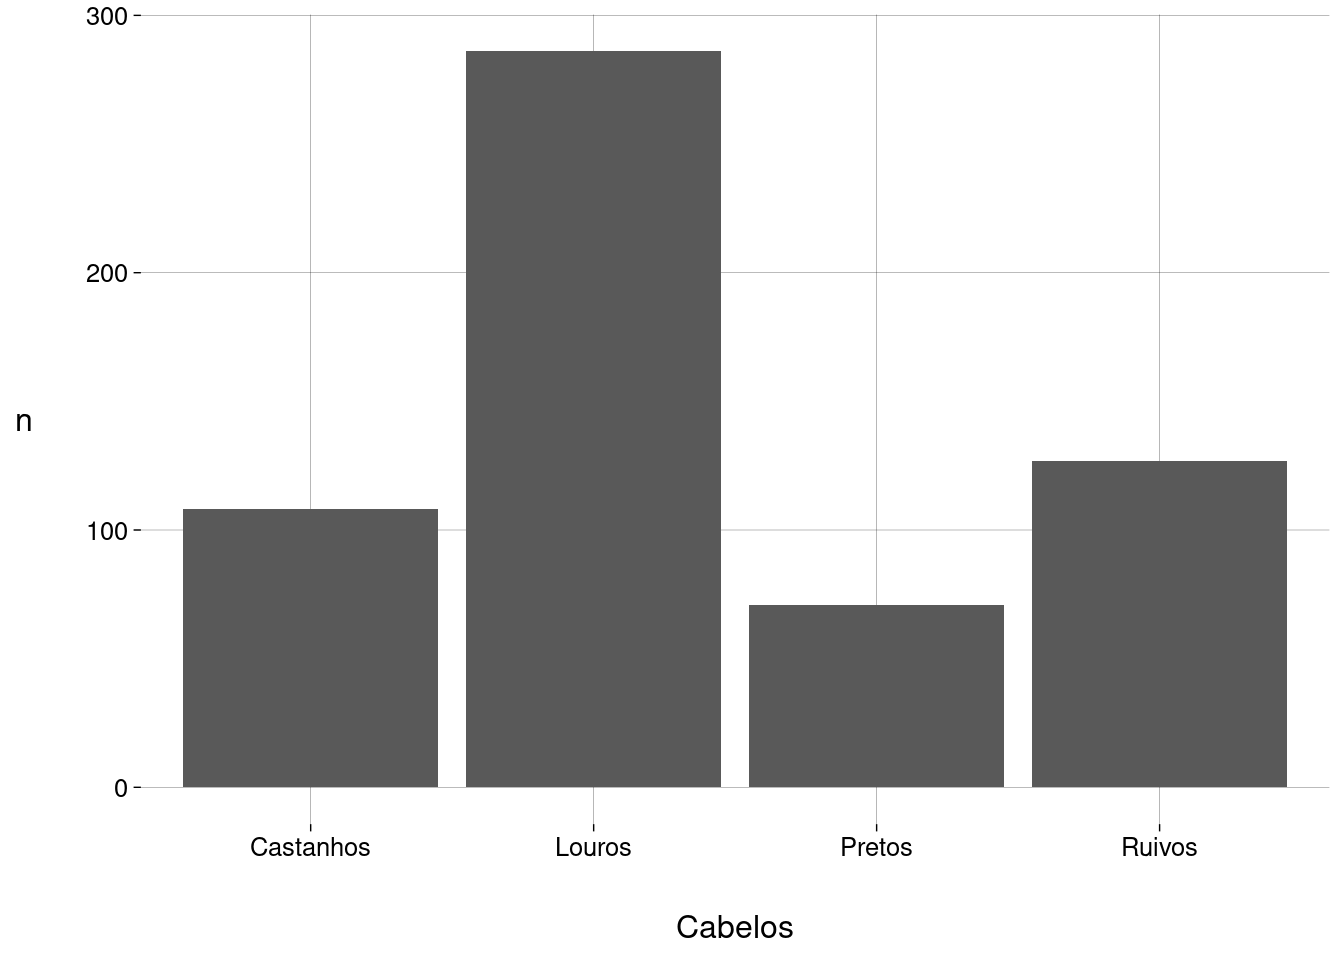
\includegraphics[width=1\linewidth]{_main_files/figure-latex/unnamed-chunk-78-1} \end{center}
\item
  Se a quantidade grande de pessoas louras de olhos castanhos (em comparação com pessoas louras de olhos azuis) for por causa da pintura de cabelos, então o gráfico acima mostra que as mulheres pintam os cabelos de louro com mais frequência do que os homens.
\item
  Quando facetamos por cor de cabelos, também podemos observar as mesmas diferenças entre homens e mulheres:

\begin{Shaded}
\begin{Highlighting}[]
\NormalTok{df }\SpecialCharTok{\%\textgreater{}\%} 
  \FunctionTok{ggplot}\NormalTok{(}\FunctionTok{aes}\NormalTok{(}\AttributeTok{x =}\NormalTok{ sexo, }\AttributeTok{fill =} \FunctionTok{fct\_infreq}\NormalTok{(olhos))) }\SpecialCharTok{+}
    \FunctionTok{geom\_bar}\NormalTok{(}\AttributeTok{position =} \StringTok{\textquotesingle{}dodge\textquotesingle{}}\NormalTok{) }\SpecialCharTok{+}
    \FunctionTok{facet\_wrap}\NormalTok{(}\SpecialCharTok{\textasciitilde{}}\NormalTok{cabelos, }\AttributeTok{labeller =}\NormalTok{ label\_both) }\SpecialCharTok{+}
    \FunctionTok{scale\_fill\_discrete}\NormalTok{(}\AttributeTok{type =} \FunctionTok{c}\NormalTok{(}\StringTok{\textquotesingle{}brown\textquotesingle{}}\NormalTok{, }\StringTok{\textquotesingle{}blue\textquotesingle{}}\NormalTok{, }\StringTok{\textquotesingle{}\#908050\textquotesingle{}}\NormalTok{, }\StringTok{\textquotesingle{}green\textquotesingle{}}\NormalTok{)) }\SpecialCharTok{+}
    \FunctionTok{labs}\NormalTok{(}
      \AttributeTok{x =} \ConstantTok{NULL}\NormalTok{,}
      \AttributeTok{y =} \ConstantTok{NULL}\NormalTok{,}
      \AttributeTok{fill =} \StringTok{\textquotesingle{}olhos\textquotesingle{}}\NormalTok{,}
      \AttributeTok{title =} \StringTok{\textquotesingle{}Cor dos olhos e sexo por cor dos cabelos\textquotesingle{}}
\NormalTok{    )}
\end{Highlighting}
\end{Shaded}

  \begin{center}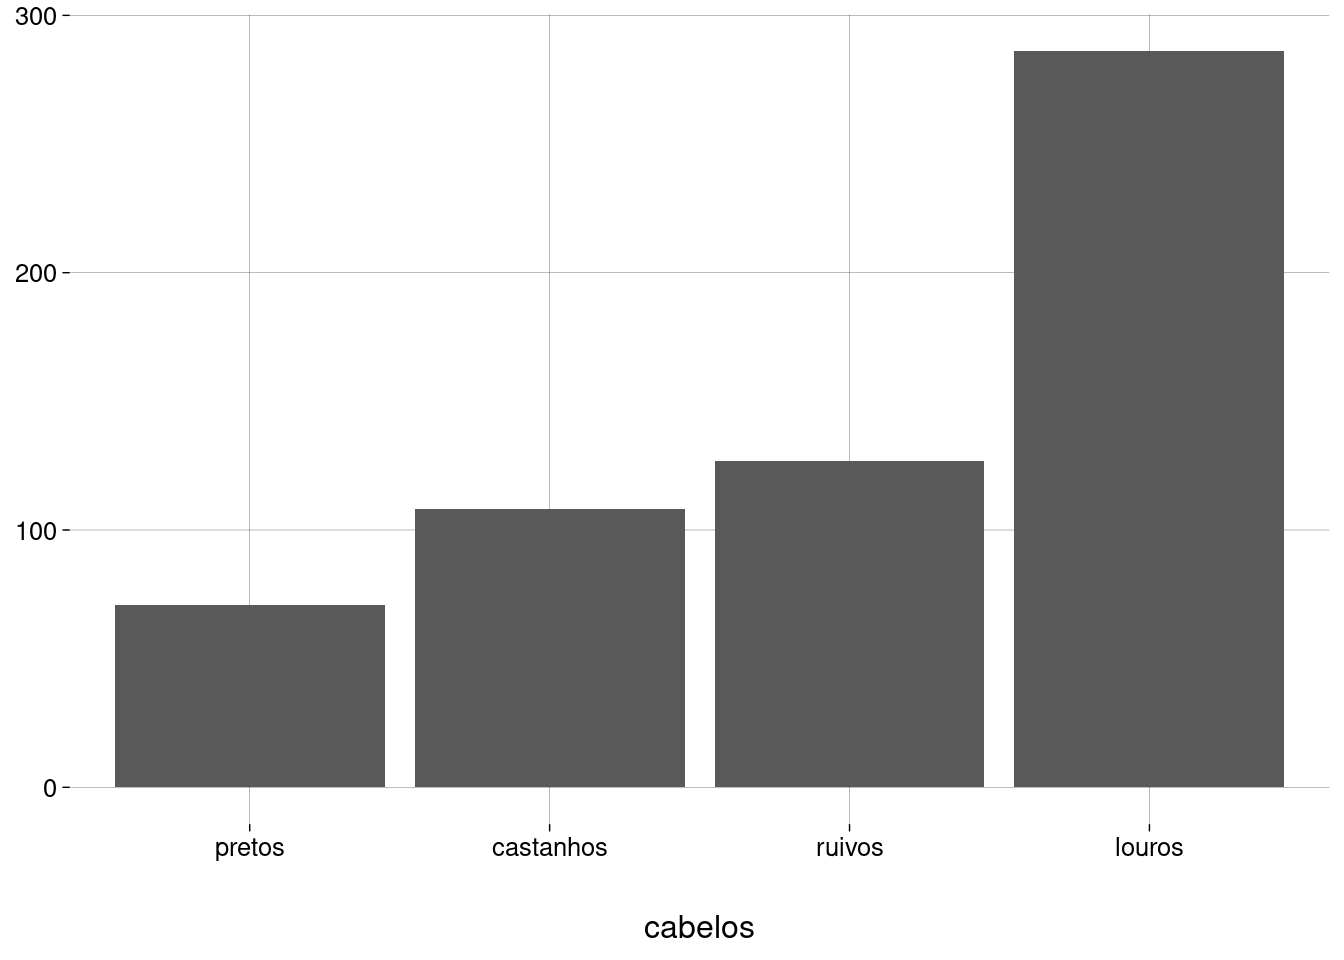
\includegraphics[width=1\linewidth]{_main_files/figure-latex/unnamed-chunk-79-1} \end{center}
\end{itemize}

\hypertarget{data-frame-juxe1-contendo-os-totais}{%
\subsection{\texorpdfstring{\emph{Data frame} já contendo os totais}{Data frame já contendo os totais}}\label{data-frame-juxe1-contendo-os-totais}}

\begin{itemize}
\item
  Você percebeu que {\hl{\texttt{geom\_bar} analisa o \emph{data frame} e calcula as frequências}} necessárias para construir o gráfico.
\item
  Em algumas situações, {\hl{o \emph{data frame} já contém as frequências}} (em vez de conter uma linha por indivíduo).
\item
  Vamos usar \texttt{count} para criar um \emph{data frame} assim:

\begin{Shaded}
\begin{Highlighting}[]
\NormalTok{df\_tot }\OtherTok{\textless{}{-}}\NormalTok{ df }\SpecialCharTok{\%\textgreater{}\%} 
  \FunctionTok{count}\NormalTok{(sexo, cabelos, olhos)}

\NormalTok{df\_tot}
\DocumentationTok{\#\# \# A tibble: 32 x 4}
\DocumentationTok{\#\#   sexo  cabelos   olhos         n}
\DocumentationTok{\#\#   \textless{}chr\textgreater{} \textless{}chr\textgreater{}     \textless{}chr\textgreater{}     \textless{}int\textgreater{}}
\DocumentationTok{\#\# 1 homem castanhos avelã        10}
\DocumentationTok{\#\# 2 homem castanhos azuis        11}
\DocumentationTok{\#\# 3 homem castanhos castanhos    32}
\DocumentationTok{\#\# 4 homem castanhos verdes        3}
\DocumentationTok{\#\# 5 homem louros    avelã        25}
\DocumentationTok{\#\# 6 homem louros    azuis        50}
\DocumentationTok{\#\# \# ... with 26 more rows}
\end{Highlighting}
\end{Shaded}
\item
  Para $4$ cores de cabelo, $4$ cores de olhos, e $2$ sexos, são $32$ combinações possíveis.
\item
  Com este \emph{data frame}, podemos gerar todos os gráficos anteriores usando {\hl{\texttt{geom\_col} no lugar de \texttt{geom\_bar}}}. Por exemplo:

\begin{Shaded}
\begin{Highlighting}[]
\NormalTok{df\_tot }\SpecialCharTok{\%\textgreater{}\%} 
  \FunctionTok{ggplot}\NormalTok{(}\FunctionTok{aes}\NormalTok{(}\AttributeTok{x =}\NormalTok{ cabelos, }\AttributeTok{y =}\NormalTok{ n)) }\SpecialCharTok{+}
    \FunctionTok{geom\_col}\NormalTok{() }\SpecialCharTok{+}
    \FunctionTok{labs}\NormalTok{(}
      \AttributeTok{y =} \ConstantTok{NULL}
\NormalTok{    )}
\end{Highlighting}
\end{Shaded}

  \begin{center}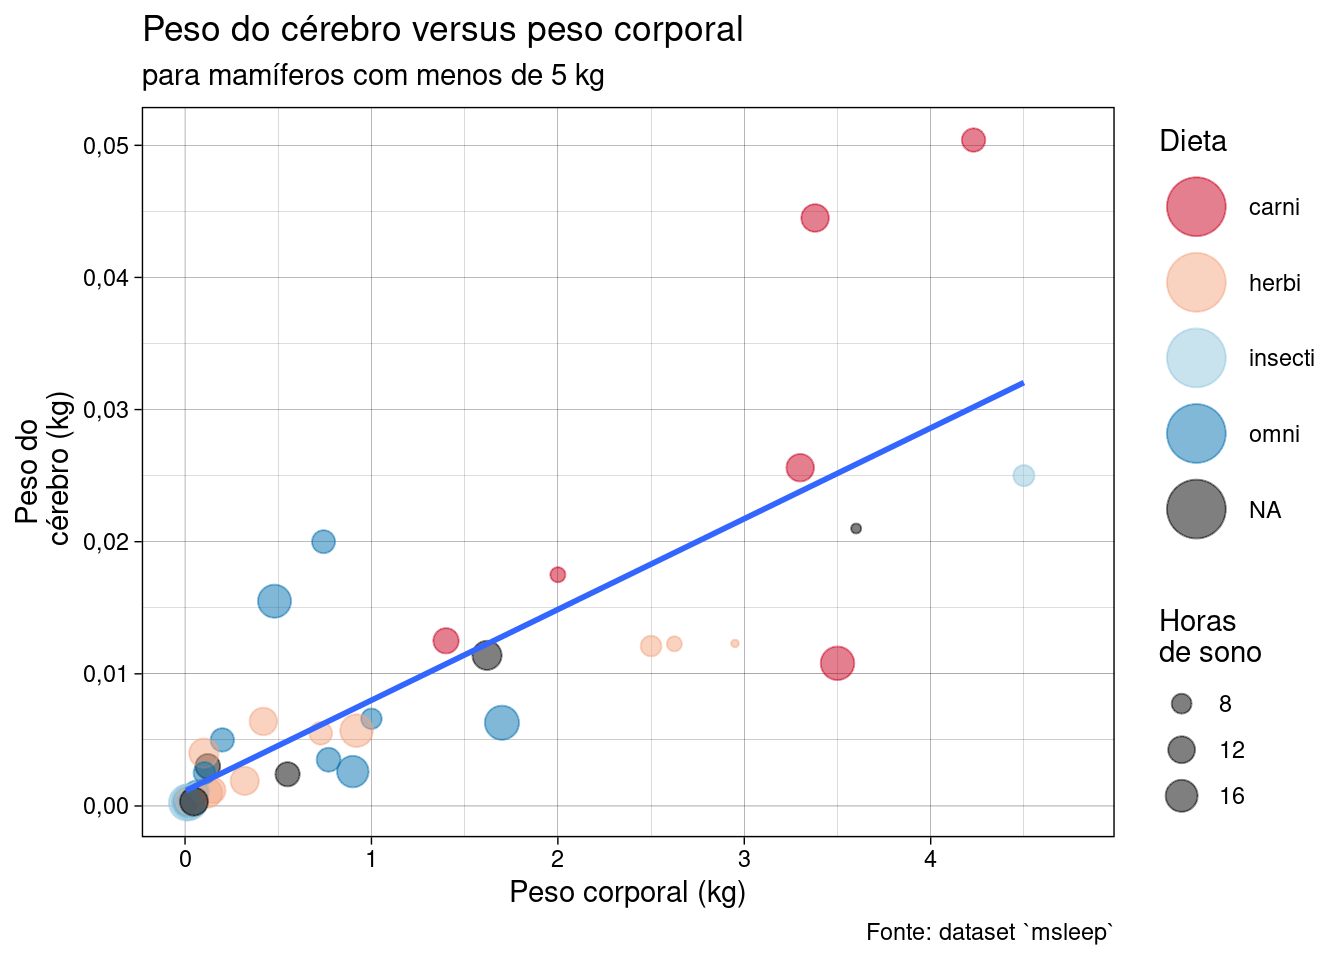
\includegraphics[width=1\linewidth]{_main_files/figure-latex/unnamed-chunk-81-1} \end{center}
\item
  Com \texttt{geom\_col}, {\hl{precisamos passar a estética $y$}} (no nosso exemplo, a variável \texttt{n}, que contém as frequências).
\item
  Para ordenar as barras, usamos a função \texttt{fct\_reorder}, que ordena os níveis de um fator (\texttt{cabelos}) de acordo com o resultado de uma função (\texttt{sum}) aplicada sobre os valores de outra variável (\texttt{n}):

\begin{Shaded}
\begin{Highlighting}[]
\NormalTok{df\_tot }\SpecialCharTok{\%\textgreater{}\%} 
  \FunctionTok{ggplot}\NormalTok{(}\FunctionTok{aes}\NormalTok{(}\AttributeTok{x =} \FunctionTok{fct\_reorder}\NormalTok{(cabelos, n, sum), }\AttributeTok{y =}\NormalTok{ n)) }\SpecialCharTok{+}
    \FunctionTok{geom\_col}\NormalTok{() }\SpecialCharTok{+}
    \FunctionTok{labs}\NormalTok{(}
      \AttributeTok{x =} \StringTok{\textquotesingle{}cabelos\textquotesingle{}}\NormalTok{,}
      \AttributeTok{y =} \ConstantTok{NULL}
\NormalTok{    )}
\end{Highlighting}
\end{Shaded}

  \begin{center}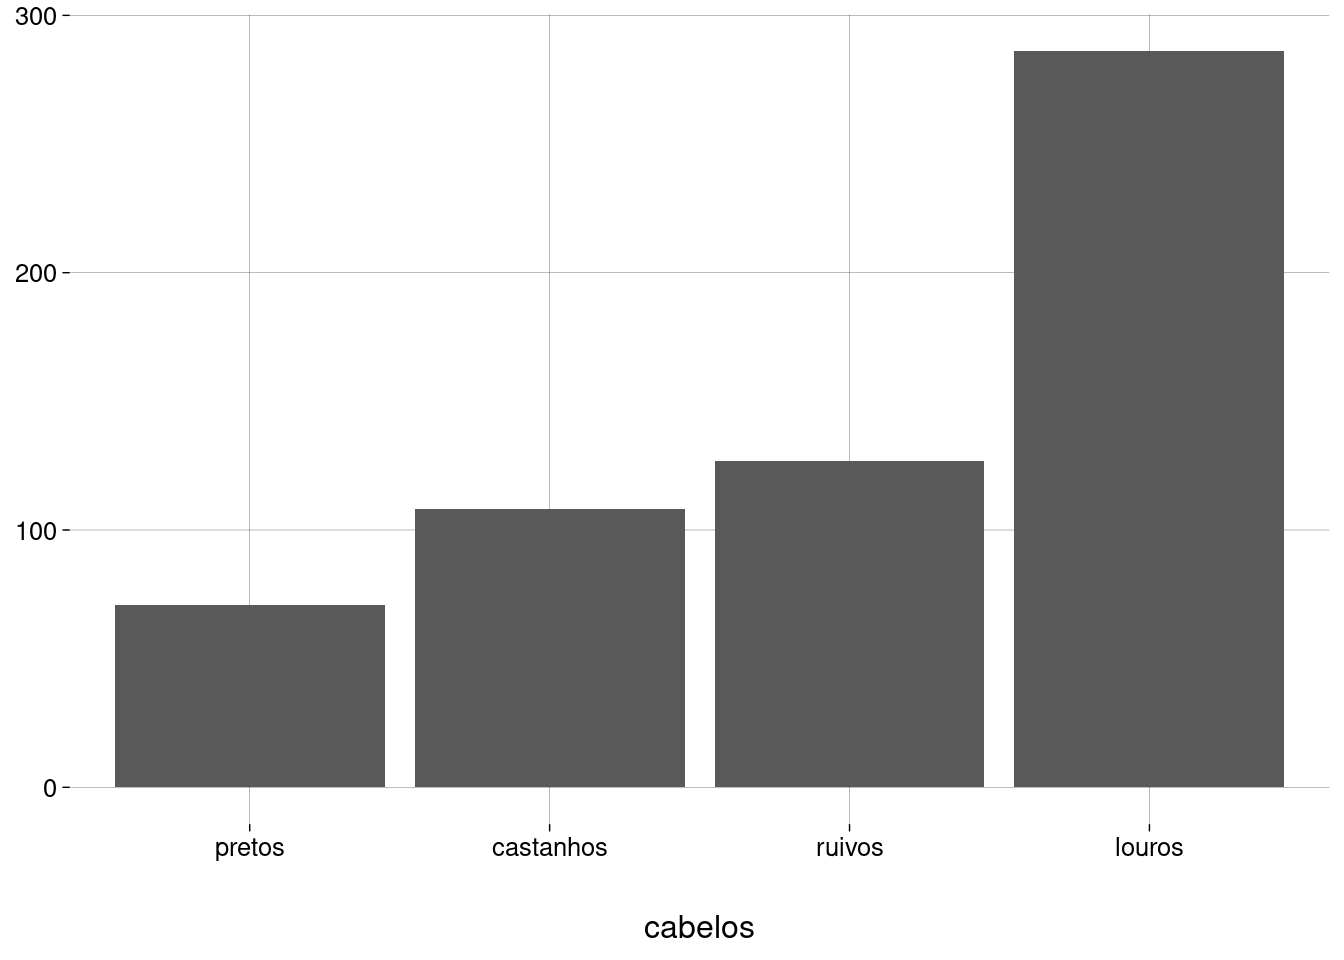
\includegraphics[width=1\linewidth]{_main_files/figure-latex/unnamed-chunk-82-1} \end{center}
\end{itemize}

\hypertarget{gruxe1ficos-de-linha-e-suxe9ries-temporais}{%
\section{Gráficos de linha e séries temporais}\label{gruxe1ficos-de-linha-e-suxe9ries-temporais}}

\hypertarget{conjunto-de-dados-3}{%
\subsection{Conjunto de dados}\label{conjunto-de-dados-3}}

\begin{itemize}
\item
  O R tem uma matriz com as quantidades de telefones em várias regiões do mundo ao longo de vários anos:

\begin{Shaded}
\begin{Highlighting}[]
\NormalTok{WorldPhones}
\DocumentationTok{\#\#      N.Amer Europe Asia S.Amer Oceania Africa Mid.Amer}
\DocumentationTok{\#\# 1951  45939  21574 2876   1815    1646     89      555}
\DocumentationTok{\#\# 1956  60423  29990 4708   2568    2366   1411      733}
\DocumentationTok{\#\# 1957  64721  32510 5230   2695    2526   1546      773}
\DocumentationTok{\#\# 1958  68484  35218 6662   2845    2691   1663      836}
\DocumentationTok{\#\# 1959  71799  37598 6856   3000    2868   1769      911}
\DocumentationTok{\#\# 1960  76036  40341 8220   3145    3054   1905     1008}
\DocumentationTok{\#\# 1961  79831  43173 9053   3338    3224   2005     1076}
\end{Highlighting}
\end{Shaded}
\item
  Os números representam milhares.
\item
  {\hl{Os números dos anos são os nomes das linhas da matriz.}}
\item
  Vamos transformar esta matriz em uma \emph{tibble}:

\begin{Shaded}
\begin{Highlighting}[]
\NormalTok{fones }\OtherTok{\textless{}{-}}\NormalTok{ WorldPhones }\SpecialCharTok{\%\textgreater{}\%} 
  \FunctionTok{as\_tibble}\NormalTok{(}\AttributeTok{rownames =} \StringTok{\textquotesingle{}Ano\textquotesingle{}}\NormalTok{) }\SpecialCharTok{\%\textgreater{}\%} 
  \FunctionTok{mutate}\NormalTok{(}\AttributeTok{Ano =} \FunctionTok{as.numeric}\NormalTok{(Ano))}

\NormalTok{fones}
\DocumentationTok{\#\# \# A tibble: 7 x 8}
\DocumentationTok{\#\#     Ano N.Amer Europe  Asia S.Amer Oceania Africa Mid.Amer}
\DocumentationTok{\#\#   \textless{}dbl\textgreater{}  \textless{}dbl\textgreater{}  \textless{}dbl\textgreater{} \textless{}dbl\textgreater{}  \textless{}dbl\textgreater{}   \textless{}dbl\textgreater{}  \textless{}dbl\textgreater{}    \textless{}dbl\textgreater{}}
\DocumentationTok{\#\# 1  1951  45939  21574  2876   1815    1646     89      555}
\DocumentationTok{\#\# 2  1956  60423  29990  4708   2568    2366   1411      733}
\DocumentationTok{\#\# 3  1957  64721  32510  5230   2695    2526   1546      773}
\DocumentationTok{\#\# 4  1958  68484  35218  6662   2845    2691   1663      836}
\DocumentationTok{\#\# 5  1959  71799  37598  6856   3000    2868   1769      911}
\DocumentationTok{\#\# 6  1960  76036  40341  8220   3145    3054   1905     1008}
\DocumentationTok{\#\# \# ... with 1 more row}
\end{Highlighting}
\end{Shaded}
\item
  Esta \emph{tibble} {\hl{não está no formato \emph{tidy}}}. Queremos que cada linha corresponda a uma observação, contendo

  \begin{itemize}
  \item
    Ano,
  \item
    Região,
  \item
    Quantidade de telefones.
  \end{itemize}
\item
  Usamos a função \texttt{pivot\_longer} para mudar o formato da \emph{tibble}:

\begin{Shaded}
\begin{Highlighting}[]
\NormalTok{fones\_long }\OtherTok{\textless{}{-}}\NormalTok{ fones }\SpecialCharTok{\%\textgreater{}\%} 
  \FunctionTok{pivot\_longer}\NormalTok{(}
    \AttributeTok{cols =} \SpecialCharTok{{-}}\NormalTok{Ano,}
    \AttributeTok{names\_to =} \StringTok{\textquotesingle{}Região\textquotesingle{}}\NormalTok{,}
    \AttributeTok{values\_to =} \StringTok{\textquotesingle{}n\textquotesingle{}}
\NormalTok{  )}

\NormalTok{fones\_long}
\DocumentationTok{\#\# \# A tibble: 49 x 3}
\DocumentationTok{\#\#     Ano Região      n}
\DocumentationTok{\#\#   \textless{}dbl\textgreater{} \textless{}chr\textgreater{}   \textless{}dbl\textgreater{}}
\DocumentationTok{\#\# 1  1951 N.Amer  45939}
\DocumentationTok{\#\# 2  1951 Europe  21574}
\DocumentationTok{\#\# 3  1951 Asia     2876}
\DocumentationTok{\#\# 4  1951 S.Amer   1815}
\DocumentationTok{\#\# 5  1951 Oceania  1646}
\DocumentationTok{\#\# 6  1951 Africa     89}
\DocumentationTok{\#\# \# ... with 43 more rows}
\end{Highlighting}
\end{Shaded}
\item
  Confira: antes, tínhamos $7$ anos, com $7$ quantidades por ano, uma quantidade por região. Eram $49$ quantidades. Agora temos uma \emph{tibble} de $49$ linhas.
\end{itemize}

\hypertarget{gerando-gruxe1ficos-de-linha}{%
\subsection{Gerando gráficos de linha}\label{gerando-gruxe1ficos-de-linha}}

\begin{itemize}
\item
  {\hl{A geometria \texttt{geom\_line} gera gráficos de linha.}} Perceba como geramos uma linha por região:

\begin{Shaded}
\begin{Highlighting}[]
\NormalTok{fones\_long }\SpecialCharTok{\%\textgreater{}\%} 
  \FunctionTok{ggplot}\NormalTok{(}\FunctionTok{aes}\NormalTok{(}\AttributeTok{x =}\NormalTok{ Ano, }\AttributeTok{y =}\NormalTok{ n, }\AttributeTok{color =}\NormalTok{ Região)) }\SpecialCharTok{+}
    \FunctionTok{geom\_line}\NormalTok{() }\SpecialCharTok{+}
    \FunctionTok{scale\_x\_continuous}\NormalTok{(}\AttributeTok{breaks =} \DecValTok{1951}\SpecialCharTok{:}\DecValTok{1961}\NormalTok{)}
\end{Highlighting}
\end{Shaded}

  \begin{center}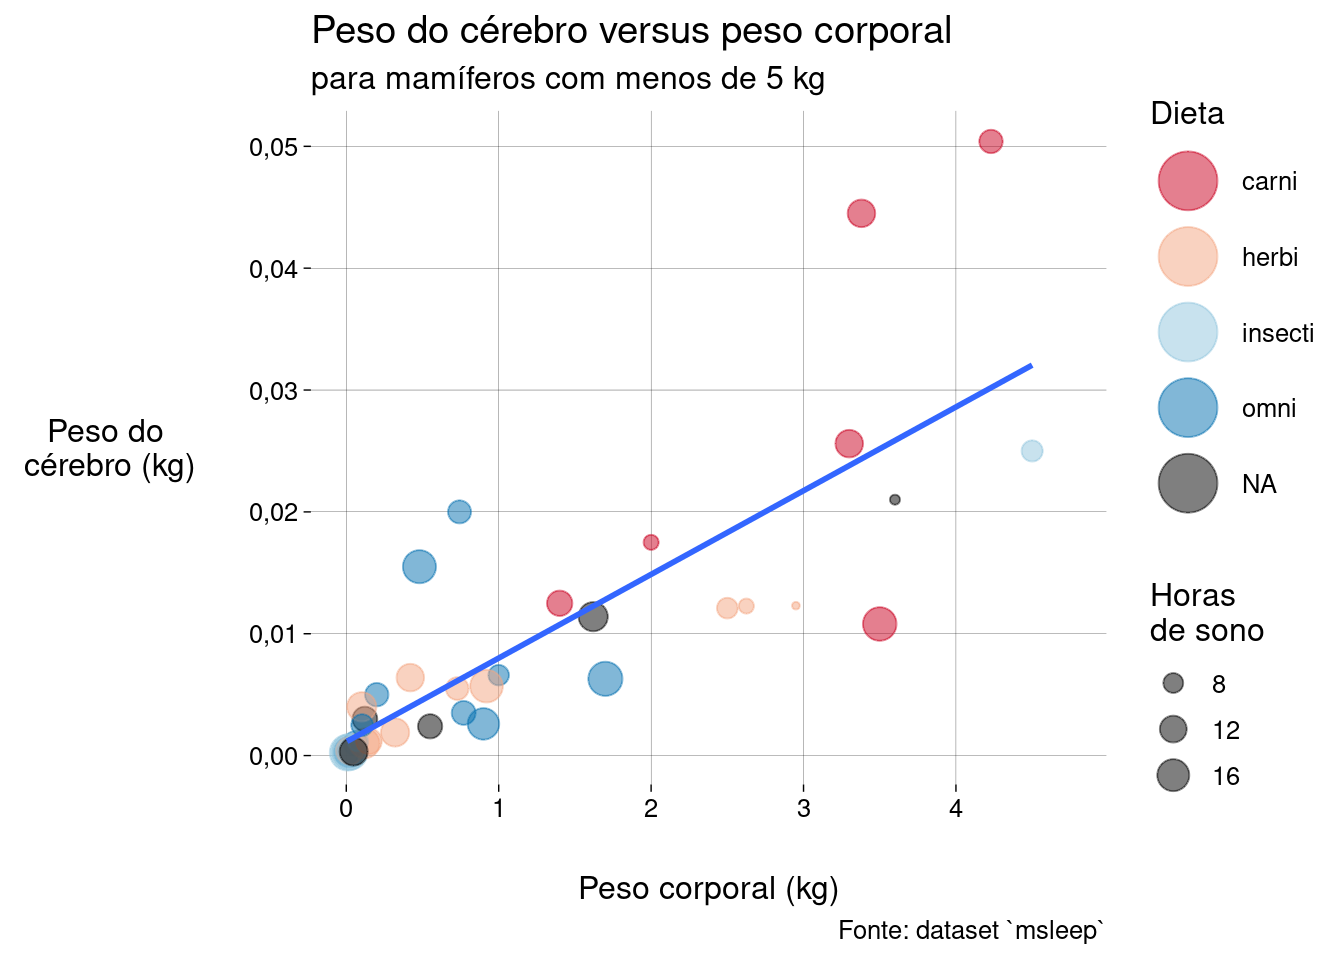
\includegraphics[width=1\linewidth]{_main_files/figure-latex/unnamed-chunk-86-1} \end{center}
\item
  Embora a legenda associe uma cor a cada região, {\hl{a leitura seria mais fácil se a ordem das regiões na legenda coincidisse com a posição das linhas na borda direita da grade}}:

\begin{Shaded}
\begin{Highlighting}[]
\NormalTok{fones\_long }\SpecialCharTok{\%\textgreater{}\%} 
  \FunctionTok{ggplot}\NormalTok{(}
      \FunctionTok{aes}\NormalTok{(}
        \AttributeTok{x =}\NormalTok{ Ano, }
        \AttributeTok{y =}\NormalTok{ n, }
        \AttributeTok{color =} \FunctionTok{fct\_rev}\NormalTok{(}\FunctionTok{fct\_reorder}\NormalTok{(Região, n, max))}
\NormalTok{      )}
\NormalTok{  ) }\SpecialCharTok{+}
    \FunctionTok{geom\_line}\NormalTok{() }\SpecialCharTok{+}
    \FunctionTok{scale\_x\_continuous}\NormalTok{(}\AttributeTok{breaks =} \DecValTok{1951}\SpecialCharTok{:}\DecValTok{1961}\NormalTok{) }\SpecialCharTok{+}
    \FunctionTok{labs}\NormalTok{(}
      \AttributeTok{color =} \StringTok{\textquotesingle{}Região\textquotesingle{}}\NormalTok{,}
      \AttributeTok{y =} \StringTok{\textquotesingle{}\textquotesingle{}}\NormalTok{,}
      \AttributeTok{x =} \ConstantTok{NULL}\NormalTok{,}
      \AttributeTok{title =} \StringTok{\textquotesingle{}Quantidade de aparelhos de telefone por ano, por região\textquotesingle{}}
\NormalTok{    )}
\end{Highlighting}
\end{Shaded}

  \begin{center}\includegraphics[width=1\linewidth]{_main_files/figure-latex/unnamed-chunk-87-1} \end{center}
\item
  Parece que está faltando uma linha, mas o que acontece é que as quantidades da América do Sul e da Oceania são bem parecidas:

\begin{Shaded}
\begin{Highlighting}[]
\NormalTok{fones\_long }\SpecialCharTok{\%\textgreater{}\%}
  \FunctionTok{filter}\NormalTok{(Região }\SpecialCharTok{\%in\%} \FunctionTok{c}\NormalTok{(}\StringTok{\textquotesingle{}S.Amer\textquotesingle{}}\NormalTok{, }\StringTok{\textquotesingle{}Oceania\textquotesingle{}}\NormalTok{)) }\SpecialCharTok{\%\textgreater{}\%} 
  \FunctionTok{ggplot}\NormalTok{(}
    \FunctionTok{aes}\NormalTok{(}
      \AttributeTok{x =}\NormalTok{ Ano, }
      \AttributeTok{y =}\NormalTok{ n, }
      \AttributeTok{color =} \FunctionTok{fct\_rev}\NormalTok{(}\FunctionTok{fct\_reorder}\NormalTok{(Região, n, max))}
\NormalTok{    )}
\NormalTok{  ) }\SpecialCharTok{+}
    \FunctionTok{geom\_line}\NormalTok{() }\SpecialCharTok{+}
    \FunctionTok{scale\_x\_continuous}\NormalTok{(}\AttributeTok{breaks =} \DecValTok{1951}\SpecialCharTok{:}\DecValTok{1961}\NormalTok{) }\SpecialCharTok{+}
    \FunctionTok{labs}\NormalTok{(}\AttributeTok{y =} \ConstantTok{NULL}\NormalTok{, }\AttributeTok{color =} \StringTok{\textquotesingle{}Região\textquotesingle{}}\NormalTok{)}
\end{Highlighting}
\end{Shaded}

  \begin{center}\includegraphics[width=1\linewidth]{_main_files/figure-latex/unnamed-chunk-88-1} \end{center}
\item
  Estamos tratando estes dados como simples números, mas, na verdade, {\hl{este conjunto de dados é uma série temporal (\emph{time series})}}.
\item
  R tem todo um conjunto de funções para tratar séries temporais, calcular tendências, achar padrões cíclicos, fazer estimativas, e gerar gráficos específicos, entre outras coisas.
\item
  Mas não vamos falar mais sobre séries temporais aqui.
\item
  O {\hl{pacote \texttt{tsibble}}} oferece maneiras de trabalhar com séries temporais de maneira \emph{tidy}. Você pode ler a documentação do pacote entrando

\begin{Shaded}
\begin{Highlighting}[]
\FunctionTok{library}\NormalTok{(tsibble)}
\NormalTok{?}\StringTok{\textasciigrave{}}\AttributeTok{tsibble{-}package}\StringTok{\textasciigrave{}}
\end{Highlighting}
\end{Shaded}
\end{itemize}

\hypertarget{exercuxedcios-4}{%
\section{Exercícios}\label{exercuxedcios-4}}

Em breve.

\hypertarget{referuxeancias-sobre-visualizauxe7uxe3o-e-r}{%
\section{Referências sobre visualização e R}\label{referuxeancias-sobre-visualizauxe7uxe3o-e-r}}

\begin{rmdtip}
Busque mais informações sobre os pacotes \texttt{tidyverse} e \texttt{ggplot2} \protect\hyperlink{refrec}{nas referências recomendadas}.

\end{rmdtip}

\hypertarget{medidas}{%
\chapter{Medidas}\label{medidas}}

\end{document}
